\documentclass[11pt]{article}
\usepackage[a4paper,margin=0.85in]{geometry}
\usepackage[T1]{fontenc}
\usepackage{lmodern}
\usepackage{amsmath,amssymb,textcomp}
\usepackage{booktabs,longtable,array,tabularx}
\newcolumntype{L}{>{\raggedright\arraybackslash}X}
\usepackage{pdflscape}
\usepackage{graphicx}
\usepackage[numbers,sort&compress]{natbib}
\usepackage{hyperref}
\hypersetup{
  colorlinks=true, linkcolor=black, citecolor=black, urlcolor=blue,
  pdftitle={Native 1-Bit and 1.58-Bit Large Language Models: A Survey and an Independent Re-Evaluation},
  pdfauthor={Habib Ullah Manzoor and Basim Alhumaily},
  pdfsubject={Survey and independent re-evaluation of native 1-bit and 1.58-bit large language models},
  pdfkeywords={1-bit language models, 1.58-bit language models, BitNet, quantization-aware training, efficient inference, hardware co-design}
}
\usepackage{microtype}
\usepackage{caption}
\usepackage{authblk}
\captionsetup{font=small,labelfont=bf,skip=4pt}
\graphicspath{{figures/}}
\setcounter{secnumdepth}{3}
\title{Native 1-Bit and 1.58-Bit Large Language Models:\\[2pt]
 A Survey and an Independent Re-Evaluation}
\author[1]{Habib Ullah Manzoor\thanks{Corresponding author. Email: \texttt{habib.manzoor@uws.ac.uk}}}
\author[2]{Basim Alhumaily\thanks{Email: \texttt{b.alhumaily@qu.edu.sa}}}
\affil[1]{School of Computing, Engineering and Physical Sciences, University of the West of Scotland, UK}
\affil[2]{Department of Electrical Engineering, College of Engineering, Qassim University, Buraydah 52571, Saudi Arabia}
\date{}
\begin{document}
\maketitle
\begin{abstract}
\noindent Large language models whose linear-layer weights are constrained to
binary $\{-1,+1\}$ or ternary $\{-1,0,+1\}$ turn the dominant matrix
multiplication into addition. The centre of gravity is the native paradigm, which
imposes that constraint during training; adjacent post-training and
quantization-aware routes target the same one-to-two-bit range. This paper is a curated,
open-access survey of 135 works from 2023 to 2026, organized on a taxonomy and a common
effective-bits accounting, together with an independent re-measurement of the flagship
open model's headline claims and, where open matched checkpoints exist, a controlled test
of the accuracy claim. In a matched comparison, a native ternary model against its FP16
counterpart at the same parameter count, tokenizer, and training data, the two land
within 0.6 points on a seven-task zero-shot suite at the two-billion-parameter scale,
with the ternary model's perplexity about 14\% higher: downstream parity, worse
language-modeling loss. Post-hoc 4-bit quantization of a full-precision model loses more
of the suite than that, and a 1.58-bit model at the one-billion-parameter scale loses
much more; this is consistent with, but too thin a basis alone to establish, a scale
dependence for the parity result, and whether it holds beyond the measured regime is
untested. On efficiency the finding is pointed: on
one commodity x86 machine a standard 4-bit quantization of the full-precision baseline
matched or beat the flagship 1-bit model on decode speed and on-disk size and was
comparable on per-token energy, and held close on the accuracy tasks checked, leaving the
1-bit model only a 24-to-27\% smaller resident set; its efficiency case at this scale
holds against half precision and an 8-bit baseline but not against 4-bit, and a GPU and a
second machine are untested. The reference CPU
runtime, moreover, does not run the flagship model correctly as documented, needing a
one-line activation fix, a sign the open deployment path is still immature. The
activation-precision floor and training stability at frontier scale remain the field's
open problems.
\end{abstract}

\noindent\textbf{Index Terms:} 1-bit and 1.58-bit language models, BitNet,
quantization-aware training, efficient inference, hardware co-design.
\medskip

%% ===== 01-introduction
\section{Introduction}

\subsection{The inference wall}

The dominant cost of a deployed large language model (LLM) is no longer training but
inference. Every generated token requires a full forward pass, and for autoregressive
decoding that pass is bounded not by arithmetic throughput but by the movement of
weights from memory into the compute units. Accelerator peak throughput, measured in
floating-point operations per second, has grown far faster than dynamic-memory bandwidth
for a decade: as the Spectra analysis notes, GPU operations per second have
doubled roughly every 1.26 years against every 2.9 years for memory bandwidth
\cite{Kaushal2024-Spectra}. The arithmetic-to-bandwidth ratio of hardware
has therefore drifted steadily away from what dense half-precision inference requires. The practical
consequences are by now familiar: multi-GPU servers are needed for models that would
otherwise fit on a single card; inference energy budgets draw scrutiny on
sustainability grounds; and running a capable model on a phone, a laptop, or an
embedded board without a network round trip remains largely infeasible.

Quantization addresses this wall directly by reducing the number of bits per weight,
and hence the number of bytes that must cross the memory hierarchy. Eight-bit and
four-bit post-training quantization are now routine. Below four bits, however, accuracy
degrades sharply for models that are quantized after training \cite{Huang2024-BiLLM},
\cite{Shang2023-PBLLM}, and a growing body of scaling-law analysis indicates that this
degradation is not a transient engineering problem. For a fixed architecture, the loss
added by low-bit quantization grows with the number of training tokens, so that the
better trained the base model, the worse post-hoc compression treats it
\cite{Ouyang2024-QiDScaling,Kumar2024-ScalingLawsPrecision}.

\subsection{The native 1-bit paradigm}

A separate line of work avoids that ceiling by making the low-bit constraint part of
the model from the first optimization step. BitNet introduced the \texttt{BitLinear} layer, a
drop-in replacement for a standard linear layer that binarizes weights in the forward
pass and trains through the non-differentiable quantizer using a straight-through
estimator. The resulting 1-bit Transformers follow a loss-versus-scale curve parallel
to that of full-precision models \cite{Wang2023-BitNet,Wang2025-BitNetJMLR}. BitNet b1.58
then moved from binary weights in the set \{-1,+1\} to ternary weights in \{-1,0,+1\},
which carry $\log_2 3 \approx 1.58$ bits of information per parameter, and reported
parity with a half-precision Transformer of equal size and training-token budget from
roughly the 3B-parameter scale upward, at a fraction of the memory, latency, and energy
\cite{Ma2024-BitNetB158}. In 2025 this became concrete with BitNet b1.58 2B4T, an openly
released 2B-parameter model trained natively on 4T tokens that matches similarly sized
full-precision open models on standard benchmarks \cite{Ma2025-BitNet2B4T}.

A native 1-bit model is defined by when the low-bit constraint is imposed, during
training rather than after, which is what lets it reach an accuracy a post-hoc
quantization of the same architecture does not (Section 8.2). The inference-time
arithmetic benefit is a separate property of the resulting representation, not of how
the weights got there: whenever every weight lies in \{-1,0,+1\}, whether from native
training or post-hoc quantization, the multiplication in a matrix-vector
product disappears: each output element is an accumulation of additions and
subtractions of activation values, gated by the sign of the weight. This removes the
multiplier, which is the largest and most power-hungry component of a digital
multiply-accumulate unit, from the inner loop, and it changes what the ideal hardware
looks like \cite{Malekar2024-MatmulOrNot,Zhu2024-MatmulFree}. It also shifts the binding
constraint. Once weights occupy roughly one bit, activation precision and the memory
traffic of the key-value (KV) cache dominate, which is why the frontier of the field
has moved toward four-bit and lower activations and toward three-bit KV caches
\cite{Wang2024-BitNetA48,Wang2025-BitNetV2}.

\subsection{Related surveys}

The literature has grown from a handful of papers in 2023 to a steady stream through
2026, spanning native pre-training recipes, post-training routes toward one bit,
optimization theory, inference kernels, and a first wave of custom accelerators
(Fig. \ref{fig:timeline}). Three existing surveys touch this area. Gong et al.
\cite{Gong2024-SurveyLowbit} review low-bit LLMs broadly, from eight-bit integer down to
binary, with a systems-and-algorithms structure and a mid-2024 horizon. Liu et al.
\cite{Liu2025-SurveyBNNLLM} survey the binarization of LLMs; this framing under-weights
ternary representations, even though ternary is where native training has succeeded.
Hao et al. \cite{Hao2025-LowPrecTrainingSurvey} survey low-precision training across all
numerical formats in IEEE TPAMI, treating 1-bit models as one subsection and not
covering inference systems or hardware. None is scoped to the native 1-bit and 1.58-bit
paradigm as a coherent object of study. And none covers the 2025 and 2026 wave: BitNet
b1.58 2B4T, BitNet a4.8, and BitNet v2; GPU and CPU inference kernels; 1-bit embedding,
speech, and vision-language-action models; ternary mixture-of-experts; and the first
lookup-table ASICs and compute-in-ROM accelerators.

This paper adds two things the existing surveys do not. First, a single common-axis
comparison: every surveyed work is placed on a five-axis taxonomy (Section 4), and that
classification is what lets otherwise incomparable results be tabulated together,
reported accuracy in consistent columns and, more substantively, reported bit-widths
re-stated under one effective-bits accounting, so that a ``1.08-bit'' post-training method
and a genuine 1.58-bit native one can be read on the same scale (Section 8). Second, and
centrally, an independent re-measurement.

On accuracy, we run a controlled test the vendor comparisons lack: a native ternary model
against its FP16 counterpart at matched parameter count, tokenizer, and training data,
from open artifacts. At the two-billion-parameter scale the two land within 0.6 points on
a seven-task zero-shot suite, with the ternary model's perplexity about 14\% higher,
downstream parity with a worse language-modeling loss. A post-hoc 4-bit quantization
loses more of the suite than that, and a 1.58-bit model at the one-billion-parameter
scale loses much more, a pattern the paper's abstract already flags as suggestive rather
than conclusive: two data points, one of them a checkpoint pair whose training match is
undocumented (Section 10.2), cannot on their own settle whether scale is the real
explanation.

On efficiency, the finding is sharper than the literature's framing. We rebuild the
reference runtime and run the flagship open 1-bit model against half-precision, 8-bit,
and three 4-bit builds on one commodity x86 machine. Each of the three 4-bit builds
decodes at least as fast as the ternary model and is smaller on disk; the k-quant format
among them, the one we also measured for energy, is comparable on per-token energy, and
on the two accuracy tasks scored through the same runtime it holds close. The ternary
model's one retained advantage is a 24-to-27\% smaller resident set. On
this hardware, then, a 1-bit model shows no observed advantage over a standard 4-bit
quantization on
throughput or on-disk size, and no more than parity on energy; its efficiency case at
this scale holds against half precision and an 8-bit baseline but not against 4-bit, and
a GPU and a second machine are untested. The
reference runtime, moreover, does not run this model correctly as documented, applying
the wrong feed-forward activation until a one-line source fix (Section 10.3), a sign that
the open deployment path for these models is not yet mature. These are the paper's
principal findings.

\subsection{Contributions}

\begin{enumerate}
  \item \textbf{An independent re-evaluation.} For accuracy we run three pairs from open matched checkpoints, controlled to varying degrees (Section 10.3): native ternary against FP16 at a matched 2.4B parameters (within 0.6 points on a seven-task mean), a 4-bit quantization against its full-precision source, and a 1B model in 1.58-bit and bf16 form whose training match to its comparator is undocumented; and we re-measure MMLU and GSM8K, which an earlier version of the study had left out. For efficiency we rebuild the reference bitnet.cpp runtime and measure decode and prefill throughput, resident memory, and on-disk size for the flagship open 1-bit model against half-precision, 8-bit, and three 4-bit builds, on one x86 laptop. We also measure per-token battery energy against the half-precision, 8-bit, and 4-bit k-quant builds on the same machine (Section 10.4). On that machine the paradigm's advantage over half precision does not extend to any 4-bit build: each decodes at least as fast and is smaller on disk, and the k-quant format, the one we also checked for energy and for accuracy on two tasks, matches the ternary model on per-token energy and holds close on accuracy; the 1-bit model keeps only a 24-to-27\% resident-memory edge. A by-product of the exercise is a symptom worth recording: the reference runtime, built from source as its documentation describes, does not run this model correctly, applying a half-precision-era feed-forward activation where the model needs a squared-ReLU, so that a practitioner following the documented path gets near-broken output until a one-line source change (Section 10.3). The open deployment path for these models is not yet mature.
  \item \textbf{A common-axis comparison.} Reported accuracy is re-tabulated in consistent columns (still in each source's own evaluation terms), and reported bit-widths are re-stated under one effective-bits accounting (nominal code width plus the amortized cost of scales, masks, and codebooks), so that methods using incompatible setups can be read side by side (Section 8, Table 2).
  \item \textbf{A curated review and taxonomy.} We survey 135 open-access works of the native 1-bit and 1.58-bit paradigm from January 2023 to June 2026, plus five foundational works from 2013 to 2022 for context, and classify every one on a five-axis taxonomy of weight representation, training paradigm, quantized components, optimization mechanism, and systems stack, with a secondary cut by modality (Section 4, Fig. \ref{fig:taxonomy}, Table 1). This is a curated, arXiv-primary review, not a systematic one (Section 3.2).
  \item \textbf{A research agenda} stated as concrete, testable open problems: the capacity ceiling and its dependence on the training-token budget, training stability at frontier parameter scale, the activation-precision floor, a convergence theory for straight-through training, the absence of a shipping processor with a ternary matrix-multiplication primitive, and the robustness and safety profile of 1-bit models (Section 11).
\end{enumerate}

\subsection{Scope}

This paper covers the native paradigm, in which the sub-two-bit constraint is present
during training, together with the post-training and quantization-aware branches that
explicitly target 1.58 bits or fewer, the kernels and hardware that execute such models,
and the theory that explains their behavior. General sub-four-bit quantization, pruning,
distillation for speed, and long-context or serving-system work are cited only where
they bear directly on the 1-bit case.

The corpus is open-access only: for every work a freely downloadable version exists on
arXiv, in JMLR or PMLR, in the ACL Anthology, on OpenReview, on a gold open-access
journal page, or in an official model or framework repository, and a local copy has been
archived. This is a deliberate choice, so that every technical claim is re-checkable
without a paywall and so that the re-measurement of Section 10 can use the exact
released artifacts. One work met every other criterion but had no obtainable
open-access copy and was set aside; its abstract, with those of the paywalled records
the search surfaced, was checked against every major conclusion, and none would change
(Section 3).

\subsection{Organization}

Fig. \ref{fig:roadmap} maps the paper. Section 2 fixes notation and background. Section 3
states the scope and how the corpus was assembled. Section 4 presents the taxonomy. Sections 5, 6, and 7 cover architecture,
training, and inference systems. Section 8 presents the common-axis comparison. Section 9
surveys applications and extensions. Section 10 reports the independent re-evaluation,
the analytical core of the paper alongside Section 8. Section 11 sets out the open
problems, and Section 12 concludes.



\begin{figure}[htbp]
\centering
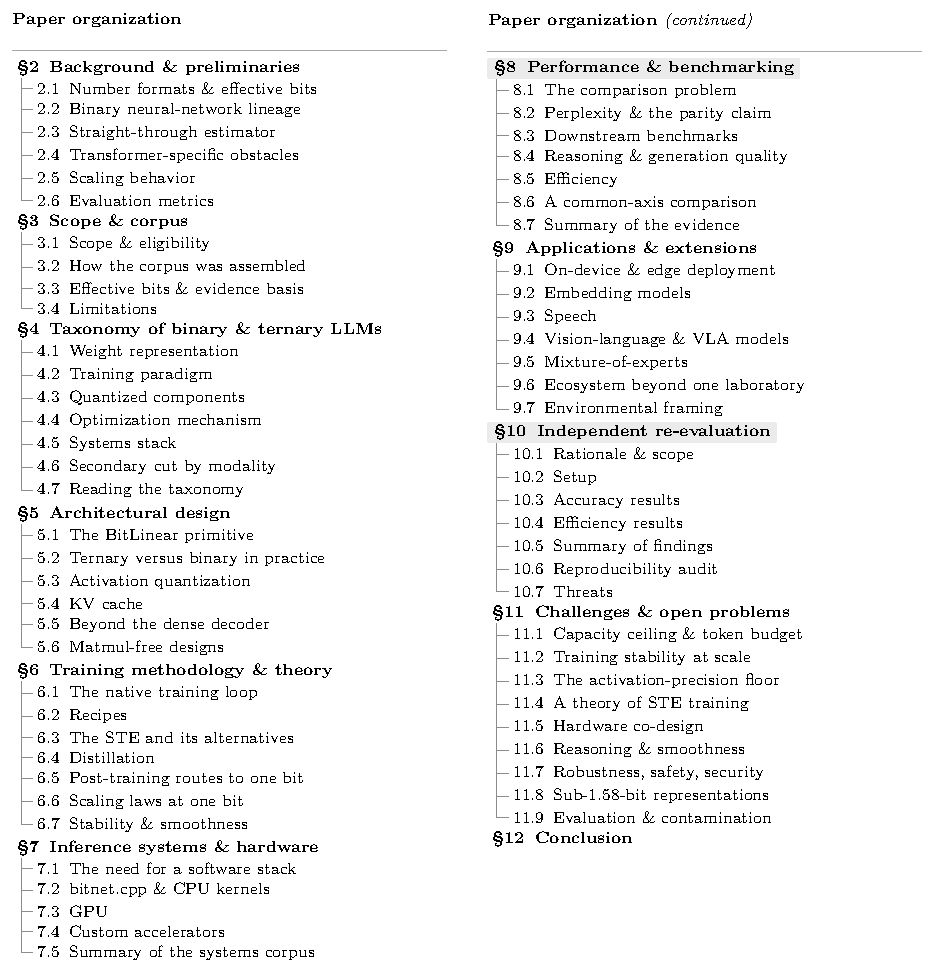
\includegraphics[width=\textwidth]{fig-roadmap.pdf}
\caption{Organization of the paper as a tree, read in two columns left to right. The shaded branches are this paper's analytical contribution.}
\label{fig:roadmap}
\end{figure}


\begin{figure}[htbp]
\centering
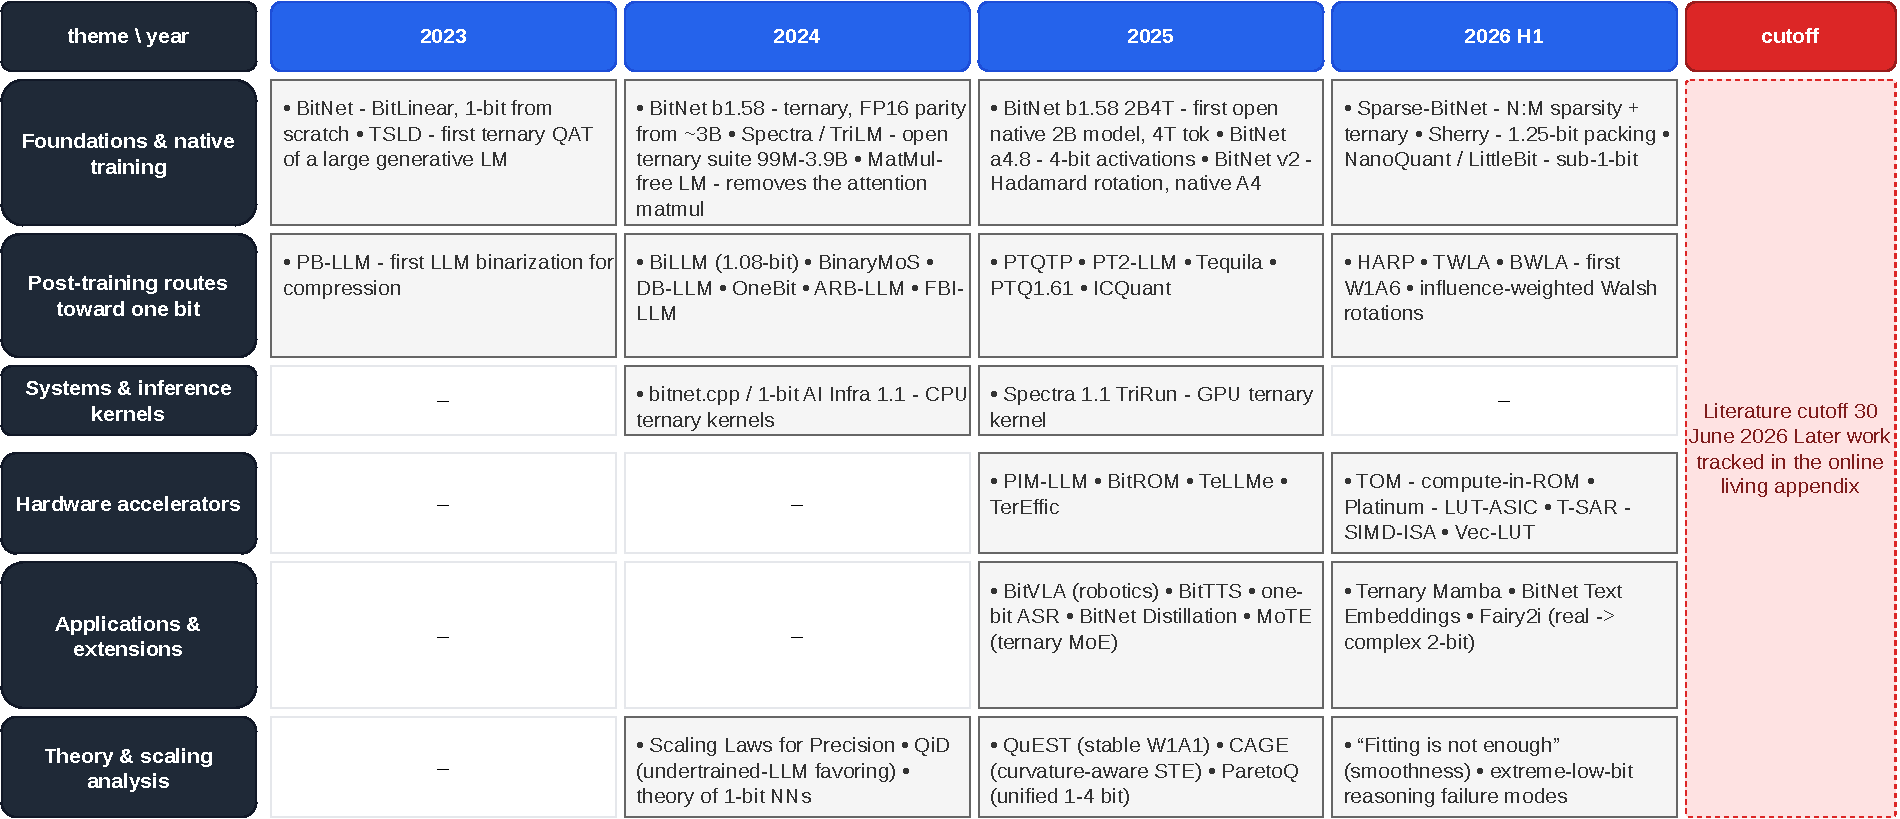
\includegraphics[width=\textwidth]{fig3-timeline.pdf}
\caption{Timeline of native 1-bit and 1.58-bit LLM research, January 2023 to June 2026, organized by theme and by year. Entries are curated highlights, not the full corpus; the full classification is Table 1.}
\label{fig:timeline}
\end{figure}



%% ===== 02-background
\section{Background and Preliminaries}

\subsection{Number formats and effective bits per weight}

A dense linear layer multiplies an input vector by a weight matrix to produce an
output vector, and that weight matrix is stored in some numeric format. Full-precision
training uses 32-bit floating point (FP32) or, in practice, the 16-bit BF16 or FP16
formats, each consisting of a sign, an exponent, and a mantissa. Integer quantization
replaces each weight with an integer code multiplied by a shared floating-point scale;
8-bit and 4-bit integer codes are the common operating points. Binary quantization
restricts the code to the two values -1 and +1, that is, one bit. Ternary quantization
restricts the code to the three values -1, 0, and +1, which carries
$\log_2 3 \approx 1.58$ bits of information and is usually stored in two bits, or in
packed schemes that approach the information bound \cite{Kaushal2024-Spectra},
\cite{Anon2026-NativeTernary}.

The reported number of bits per weight is not always the nominal code width. Partial
schemes keep a small fraction of salient columns in higher precision: BiLLM reports
about 1.08 effective bits and PB-LLM a tunable figure above one \cite{Huang2024-BiLLM},
\cite{Shang2023-PBLLM}. Structural-sparsity schemes push below one bit by storing only the
nonzero ternary positions \cite{Dong2024-STBLLM,Lee2025-LittleBit}. Packing choices for
ternary weights trade a fraction of a bit against kernel speed \cite{Vaidhya2025-Spectra11},
\cite{Huang2026-Sherry}. A consistent effective-bits accounting, defined as the code width
plus the per-weight amortized cost of scales, masks, and codebooks, is therefore a
prerequisite for comparing methods; Section 8 adopts one.

The benefit of a small integer code width is memory and bandwidth. A 2B-parameter model occupies four
to five GB in BF16 and about 0.4 GB with ternary weights in a non-embedding accounting,
and because the decode step is memory-bound, it speeds up in roughly the same proportion
\cite{Ma2025-BitNet2B4T}; Section 10.4 measures the fuller resident-memory figure once the
embedding and runtime buffers are counted too. The second benefit is arithmetic. With each weight restricted to
-1, 0, or +1, the per-weight multiplication becomes a conditional add or subtract, so the
inner product reduces to a masked accumulation \cite{Malekar2024-MatmulOrNot}.

\subsection{The binary neural network lineage}

Training networks with binary weights predates LLMs. BinaryConnect binarizes weights in
the forward and backward pass while retaining a full-precision ``shadow'' copy in which
gradients accumulate, and it observes a regularizing effect
\cite{Courbariaux2015-BinaryConnect}. XNOR-Net binarizes both weights and activations so that
a convolution becomes a bitwise XNOR followed by a population count, and it introduces
per-filter scaling factors to reduce the approximation error \cite{Rastegari2016-XNORNet}.
The transfer to language models proved harder. BinaryBERT finds the loss landscape of a
directly binarized BERT too rugged to optimize and instead initializes the model by
splitting a trained half-width ternary network \cite{Bai2021-BinaryBERT}. BiBERT identifies
information loss in the forward pass and gradient-direction mismatch in the backward
pass as the two failure modes, and addresses them with an information-preserving
attention operator and a direction-matching distillation loss \cite{Qin2022-BiBERT}. Three
lessons carried into the LLM era: a full-precision shadow weight is what makes
gradient-based training of a discrete variable work; ternary is markedly easier to
optimize than binary; and distillation from a full-precision teacher is often what
closes the last accuracy gap.

\subsection{The straight-through estimator and its pathologies}

The quantizer, which maps a full-precision weight to its quantized code, is piecewise
constant, so its gradient is zero almost everywhere and training cannot back-propagate
through it. The straight-through estimator (STE) replaces that gradient with the
identity, often clipped to the quantizer's input range, so that the forward pass sees
the quantized value while the backward pass updates the shadow weight as if the
quantizer were absent \cite{Bengio2013-STE} (Fig. \ref{fig:ste}).
Practically all native 1-bit training uses a scaled STE. BitNet's \texttt{BitLinear} layer
centers the weights and divides by their mean absolute value before applying the sign
function, quantizes activations to INT8 per token, and applies the STE through both
\cite{Wang2023-BitNet,Wang2025-BitNetJMLR}. BitNet b1.58 uses an absolute-mean ternary
rule \cite{Ma2024-BitNetB158}, and small-model studies find the median a more
outlier-robust divisor \cite{Nielsen2024-Reloaded}.

The STE is biased, and the bias manifests as slow convergence and instability that
worsen as the bit-width decreases. Recent work treats the estimator itself as the
object of study. CAGE adds a curvature-aware correction term derived from a
multi-objective view of quantization-aware training (QAT) and proves convergence in the
smooth non-convex setting \cite{Tabesh2025-CAGE}. QuEST fits the weight and activation
distributions with a Hadamard normalization and an MSE-optimal grid, and it introduces
a trust gradient that minimizes the error between the quantized-state gradient and the
true gradient, reporting stable training down to one-bit weights and activations
\cite{Panferov2025-QuEST}. A further line augments the STE with zeroth-order information
\cite{Anon2025-STE-ZerothOrder}. An orthogonal alternative removes the STE entirely: Direct
Quantized Training keeps only low-precision weights and uses stochastic rounding to
carry information between steps, eliminating the shadow copy and its memory cost
\cite{Zhao2024-DQT}. For extreme fine-tuning specifically, PV-Tuning shows that the STE
assumption is suboptimal and replaces it with a representation-agnostic
coordinate-descent procedure \cite{Malinovskii2024-PVTuning}.

\subsection{Transformer-specific obstacles}

Two properties of Transformers make sub-two-bit quantization harder than the
convolutional case.

The first is activation outliers. A small number of channels in the attention output
and in the feed-forward down-projection carry values one to two orders of magnitude
larger than the rest. Quantizing weights to roughly one bit sharply increases
sensitivity to these outliers, so most 1-bit-weight methods keep activations at INT8
\cite{Ma2024-BitNetB158}. Two routes go lower. The first is a hybrid scheme: BitNet a4.8 uses
INT4 for the attention and feed-forward inputs but keeps 8 bits for the outlier-heavy
intermediate states, which it sparsifies first, reaching an effective W1.58A4
configuration with only 55\% of parameters active and a three-bit KV cache
\cite{Wang2024-BitNetA48}. The second is rotation: the \texttt{H-BitLinear} layer of BitNet v2
applies an online Hadamard transform that spreads outlier energy across coordinates
before quantization, which enables native four-bit activations \cite{Wang2025-BitNetV2}.
Learnable and data-adaptive rotations generalize the fixed Hadamard \cite{Zagitov2026-HARP},
\cite{Zhao2026-TWLA,Zhao2026-BWLA}, and the same idea drives several post-training routes
toward one-bit weights.

The second obstacle is the placement of normalization relative to the quantized
projection, which affects stability. \texttt{BitLinear} places a LayerNorm or SubLN before
quantization, and inserting an additional RMSNorm has been reported to stabilize
fine-tuning to 1.58 bits \cite{Steinmetz2025-ExtraRMSNorm}. Continual schemes that begin in
full precision and transition to 1.58-bit training part-way through pre-training must
manage loss spikes at the switch; both retaining the optimizer state and phasing in the
quantization strength mitigate them \cite{Nielsen2025-ContinualQAT}.

\subsection{Scaling behavior}

Whether the full-precision parity of BitNet b1.58 is a genuine scaling property or an
artifact of limited training-token budgets is contested, and it is central to the open
problems of Section 11. Precision-aware scaling laws model low-precision training as a
reduction of the effective parameter count and predict that post-training quantization
degrades further as the amount of pre-training data increases
\cite{Kumar2024-ScalingLawsPrecision,Ouyang2024-QiDScaling}. Against this, native ternary
suites show ternary models overtaking quantized and even full-precision models on a
bits-for-bits basis beyond about 1B parameters, with gains that grow when training data
rather than parameter count is scaled \cite{Kaushal2024-Spectra,Vaidhya2025-Spectra11}.
ParetoQ unifies one-bit to four-bit QAT in a single framework and reports a learning
transition between two and three bits, below which the representations reorganize
substantially; ternary, two-bit, and three-bit quantization occupy a comparable
size-accuracy frontier that generally beats four-bit and binary \cite{Liu2025-ParetoQ}.
Theory has begun to catch up: a kernel-limit analysis establishes a scaling law for
1-bit networks \cite{Daliri2024-Theory1bit}, and precision-expressivity trade-offs are being
formalized \cite{Anon2026-EveryBitCounts,Anon2026-ExpressivePowerWQ}.

\subsection{Evaluation metrics}

The corpus reports, with varying completeness, the following quantities. On the accuracy
side: perplexity on WikiText-2 and C4; zero-shot accuracy on ARC-Easy, ARC-Challenge,
HellaSwag, WinoGrande, PIQA, OpenBookQA, and BoolQ, usually reported as an average; and,
for instruction-tuned models at the 2B scale, MMLU, GSM8K, and HumanEval or HumanEval+.
On the systems side: decode throughput in tokens per second and time per output token;
prefill latency and time to first token; peak resident memory; and energy per token or
per inference. Cross-paper comparison is complicated by different harness versions,
prompt formats, and few-shot counts, and, on the efficiency side, by different
hardware, thread counts, and baselines, such as FP16 against INT8, or a general
inference framework against a custom kernel. Section 8 states the effective-bits
convention and the axes used to place these results on one scale, and Section 10
reports independently measured values for a subset.



\begin{figure}[htbp]
\centering
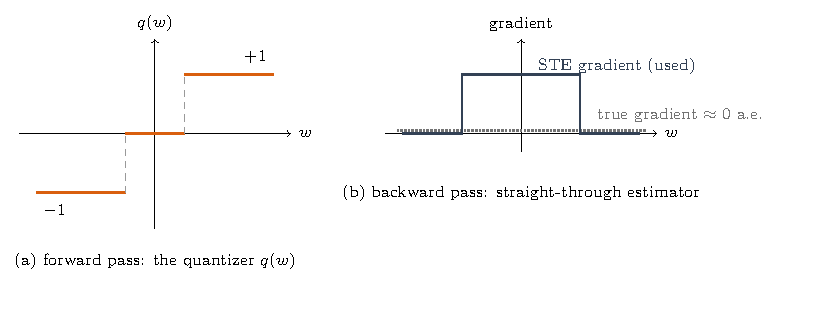
\includegraphics{fig-ste.pdf}
\caption{The straight-through estimator. (a) The forward-pass quantizer, here the ternary rule with thresholds at $\pm 0.5$ of the normalized weight $w$, is piecewise constant with zero true gradient almost everywhere. (b) The backward pass instead propagates a clipped-identity gradient (dark), letting the full-precision shadow weight update despite the quantizer's own zero gradient.}
\label{fig:ste}
\end{figure}



%% ===== 03-methodology
\section{Scope and Corpus}\label{sec:method}

\subsection{Scope and eligibility}

A work is in scope if it primarily concerns binary or ternary language models, or a
method, kernel, or hardware design that explicitly targets them. The bit-width gate is
on the \textbf{nominal or targeted} weight precision: a work is eligible if it aims at binary
weights, ternary weights, or a partial or salient-split scheme built on a sub-two-bit
backbone. The gate is deliberately not on the effective bits per weight of Section 3.3,
because that figure, which folds in the amortized cost of scales, bitmaps, and
codebooks, is itself one of the survey's findings: several eligible works turn out to
carry two to four effective bits once that cost is counted (BiLLM at about 2.88, STBLLM
at about 4.13), and re-stating those figures on a common scale is the point of Table 2,
not a reason to exclude the works. We include work first made public between January 2023
and June 2026 that makes an empirical or theoretical contribution and for which a freely
downloadable full text exists; a local copy of every included work is archived. A unified
study that sweeps a wider bit-width range, such as a one-to-four-bit
quantization-aware-training comparison, is included for its binary and ternary results
and cited only for those. Work whose method targets only three bits or more, or that has
no language-model component, is cited only where it bears directly on the binary and
ternary case; systems, analysis, and survey works that define no model of their own
appear in the tables with the weight, paradigm, and component axes marked not applicable
rather than forced into a category.
Foundational work on binary networks and the straight-through estimator from 2013 to
2022 is discussed for context and marked separately from the in-window corpus.

The open-access restriction is deliberate. It lets any reader re-check every technical
claim without a paywall, and it lets the re-evaluation of Section 10 run on the exact
released artifacts. Its cost is the possible omission of paywalled work with no preprint.
One work met every other criterion but had no obtainable open-access copy and was set
aside; its abstract, together with those of the paywalled records the search surfaced,
was checked against every principal conclusion of the paper, and none would change.

\subsection{How the corpus was assembled}

The search ran as four passes, all falling between 3 and 5 September 2026, and covers
work public on or before 30 June 2026; the final of the four, a raw arXiv API re-harvest
against the full query set, closed the window on 5 September. The primary source was
arXiv, queried through its API over cs.CL,
cs.LG, cs.AI, and cs.AR with a Boolean query over bit-width terms (``1-bit'', ``1.58-bit'',
``ternary'', ``binariz*'', ``sub-2-bit''), model terms, and technique terms (``BitNet'',
``BitLinear'', ``quantization-aware training'', ``matmul-free'', and others), plus fifteen
exact-name queries for known systems. This was supplemented by two iterations of
backward and forward citation chasing on eight seed papers through the Semantic Scholar
citation graph, by targeted web searches for named methods, and by monitoring Hugging
Face Papers and official model and framework release logs. It was not an exhaustive
multi-database search; for a fast-moving subfield that publishes predominantly as
preprints, arXiv plus citation chasing captures the frontier, and the open-access
criterion already excludes venue-only paywalled work.

Candidate records were de-duplicated, screened on title and abstract, then screened in
full text, with the open-access copy retrieved in the same pass and a failure to
retrieve treated as an exclusion. Screening removed off-topic records (most often a
primary contribution outside language modeling, such as error-correcting-code
transformers or high-energy-physics classification, with a 1-bit model as an incidental
example), records whose primary method spanned a bit-width range above two bits, and
records made public after the cutoff, which fall outside the surveyed corpus.

The flow below is the funnel for the final consolidation pass, a raw arXiv API
re-harvest with no summarizer in the loop, together with the cumulative outcome across
all four search passes. The 135 in-window primary studies are not spread
evenly over the four search years; Fig. \ref{fig:growth} gives the year-by-year count.

\begin{center}\footnotesize
\captionof*{table}{\footnotesize \textbf{Corpus-assembly funnel.} The final consolidation pass (a raw arXiv API re-harvest with no summarizer in the loop), shown with the cumulative outcome across all four search passes.}\par\medskip
\begin{tabularx}{\linewidth}{Ll}\toprule
stage & count \\
\midrule
Unique arXiv records, final raw re-harvest (core query + 15 name queries, cs.CL/LG/AI/AR, Jan 2023 to Jun 2026) & 109 \\
Already in the corpus from earlier passes & 69 \\
New, sent to full-text screening & 40 \\
New records included at full text & 15 \\
New records excluded: outside language modeling (EC-1) & 16 \\
New records excluded: bit-width range above two bits (EC-2) & 7 \\
New records excluded: duplicate or re-confirmed prior exclusion & 2 \\
Cumulative full-text eligible, all passes & 136 \\
Excluded, no obtainable open-access copy (IC-5): PT-BitNet & 1 \\
Delayed 20\% re-screen (28 sampled, 26 confirmed): removed on second reading & 1 \\
Delayed 20\% re-screen: re-included after an open-access copy was located & 1 \\
\textbf{In-window primary studies included} & \textbf{135} \\
Pre-2023 foundational works, classified in Table 1 for context & 5 \\
\textbf{Rows in Table 1} & \textbf{140} \\
Non-paper artifacts kept as dated snapshots (two model cards, one framework repository) & 3 \\
Post-cutoff records excluded from this version of the corpus & $\sim$5 \\
\bottomrule\end{tabularx}\end{center}

The re-screen removed one W4A4 scaling-law study that fails the bit-width criterion and
recovered one native-ternary encoding study once its open-access copy was found; both
revisions are in the counts above. This process departs from the frozen protocol
(\texttt{survey-protocol.md}) in three stated ways: screening was by one reviewer rather than
two, the 20\% re-screen followed the first pass by a few days rather than the two-week
washout the protocol specifies (Section 3.4), and there was no exhaustive multi-database
harvest or public pre-registration.

\subsection{Effective-bits accounting and evidence basis}

Reported bit-widths in this literature are not comparable as stated, because partial and
salient-split schemes count only the code and omit the group scales, bitmaps, and
codebooks they also store. Throughout, the \textbf{effective bits per weight} is the nominal
code width plus the per-weight amortized cost of those structures; where a source's own
strict accounting or an independent one exists, that figure is used and the basis is
noted per row in Table 2.

Rather than collapse source quality into one graded number, each work carries an
\textbf{evidence basis} made of two facts that a reader can check directly in Table 1's
``Evidence basis'' column. The first is the \textbf{venue}: a peer-reviewed conference or journal, or ``preprint''
if the only version is on arXiv or under review. The second is whether the \textbf{central result has an independent check}, meaning our own reproduction in Section 10 or a separate open study that reaches the same finding; most works have neither. Artifact
availability, whether an open model, code, or weights exist, is recorded as a free-text
note per row where known, since it could not be verified uniformly across all 140 works.

For synthesis we use a single derived split. A source is \textbf{corroborated} if it is peer reviewed or has an independent check; otherwise it is a \textbf{single unreproduced preprint}. Forty-eight of the 140 works are corroborated. This split is about the
reliability of a source and its artifacts, not about whether its headline claim is
settled: a corroborated source can still make a disputed claim. The parity claim of the
native line is the clearest example. Its sources are all corroborated, BitNet b1.58,
BitNet b1.58 2B4T, both Spectra suites, and ParetoQ, which is also at NeurIPS, and they
corroborate one another; our re-run of the released BitNet b1.58 2B4T checkpoint in
Section 10 confirms that it loads, runs, and is competitive on a common suite. None of
that tests parity at frontier scale, which remains an open problem (Section 11.1). Any
statement in the synthesis that rests only on single unreproduced preprints is marked as
such.

\subsection{Limitations}

The corpus is preprint-heavy, because the field publishes faster than journal review
cycles; this is mitigated by the corroborated-versus-single-preprint split of Section
3.3, by anchoring to peer-reviewed versions where they exist (BitNet in JMLR; OneBit,
BinaryMoS, PV-Tuning, ParetoQ, and LittleBit at NeurIPS; ARB-LLM and PT2-LLM at ICLR;
BiLLM and LC-QAT at ICML; ICQuant at COLM), and by the re-evaluation of Section 10. The search is arXiv-primary rather than exhaustive, so
open-access work in society and publisher venues with no preprint may be missed.
Screening was done by one reviewer; a re-screen of a random 20\% sample (28
studies) confirmed 26 of the 28 inclusion decisions (93\% raw intra-rater agreement), and
the two revisions it prompted are folded into the counts above. That re-screen followed
the first pass by a few days rather than the two-week washout the protocol specified, so
it measures the stability of the eligibility criteria more than blind intra-rater
agreement. One automated citation list retrieved during the
search contained unverifiable entries, which were discarded; every archived record was
confirmed against its primary source. Finally, some relevant work will appear between the
cutoff and publication; that is an inherent limitation of any fixed-cutoff survey.



\begin{figure}[htbp]
\centering
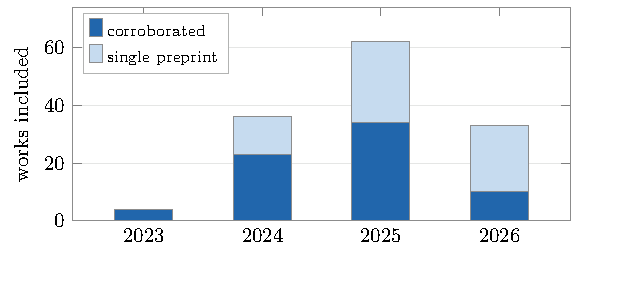
\includegraphics{fig-growth.pdf}
\caption{In-window corpus by year of first publication, stacked by evidence basis: corroborated means peer reviewed or with an independent check; the rest are single unreproduced preprints. 135 primary studies, January 2023 to June 2026 (2026 is a partial year, through the June cutoff). The falling corroborated share in recent years partly reflects review lag, not only falling scrutiny.}
\label{fig:growth}
\end{figure}



%% ===== 04-taxonomy
\section{A Taxonomy of Binary and Ternary LLMs}

A survey of this area must impose structure, because the phrase ``1-bit LLM'' is used for
at least three different research programs: training a model under a sub-two-bit
constraint from scratch, compressing a trained model down toward one bit, and building
hardware that executes ternary weights efficiently. We organize the field along five
orthogonal axes (Table 1). Four of them, weight representation, training paradigm,
quantized components, and systems stack, partition the corpus, so their category counts
sum to the full 140 works; the fifth, optimization mechanism, is a non-exclusive tally,
since one work can combine mechanisms. The axes are deliberately independent, so that a
work's position on one does not determine its position on another, and the most
influential works are those that advance the state of the art on several axes at once.

\subsection{Axis 1: weight representation}

The first choice is the value set. Binary weights, drawn from \{-1,+1\}, give the largest
nominal compression and the simplest kernel, but they cannot express the absence of a
connection. Thirty-four surveyed works are primarily binary, and most of them are
post-training or fine-tuning methods that apply the binary constraint to an
already-trained model \cite{Huang2024-BiLLM,Li2024-ARBLLM,Xu2024-OneBit},
\cite{Ma2024-FBILLM}. Ternary weights, drawn from \{-1,0,+1\}, add a zero state. This both
restores sparsity, since roughly 40\% to 60\% of weights go to zero in practice, and
makes optimization markedly easier in experiments. Sixty-two works are ternary, and
this is where native from-scratch training has succeeded \cite{Ma2024-BitNetB158},
\cite{Kaushal2024-Spectra,Zhu2024-MatmulFree}; an early instance, predating BitNet,
demonstrated the first ternary and binary sequence-to-sequence Transformers for
summarization and machine translation \cite{Liu2023-BinTernNLG}. Mixed or partial schemes, of which there
are 21, keep a small set of salient columns, or a low-rank residual branch, in higher
precision. Examples are the roughly 1.08 effective bits of BiLLM \cite{Huang2024-BiLLM}, the
tunable fraction of PB-LLM \cite{Shang2023-PBLLM}, the dedicated high-precision expert
branch of pQuant \cite{Zhang2026-pQuant}, and the saliency-graph-guided scaling of SAGE-PTQ
\cite{Abdalla2026-SAGEPTQ}; each trades a fraction of a bit for a substantial accuracy
recovery. A small but distinct line uses complex-valued weights in
$\{\pm 1, \pm i\}$, which costs two bits of storage but supports multiplication-free
accumulation \cite{Wang2025-iFairy,Wang2025-Fairy2i}. The remaining 23 works, kernels,
accelerators, theory, and surveys, define no weight format of their own and are counted
separately in Fig. \ref{fig:taxonomy}.

\subsection{Axis 2: training paradigm}

The second choice is when the low-bit constraint enters. Native from-scratch training,
in 27 works, places a quantizer in \texttt{BitLinear} from the first optimization step; this is
the defining paradigm of the survey and the one that has demonstrated full-precision
parity at scale \cite{Wang2023-BitNet,Ma2024-BitNetB158,Ma2025-BitNet2B4T},
\cite{Kaushal2024-Spectra}. Continual quantization-aware pre-training, in 2 works, begins in
full precision and transitions to 1.58-bit training part-way through, which reduces
total cost but introduces a loss spike at the switch that must be managed
\cite{Nielsen2025-ContinualQAT,Tu2025-Rethink1bitOpt}. Quantization-aware fine-tuning, in
37 works, inserts the quantizer into a fine-tuning or short continued-training loop over
a pretrained full-precision model \cite{Xu2024-OneBit,Du2024-BitDistiller},
\cite{Wu2025-BitNetDistillation}. Post-training quantization, in 30 works, uses only a
calibration set and no gradient updates \cite{Huang2024-BiLLM,Li2024-ARBLLM},
\cite{Xiao2025-PTQTP,Yan2025-PT2LLM,Xu2024-CRVQ,Edalati2024-OAC}. At a fixed
bit-width, the accuracy ordering is
generally native, then quantization-aware training, then post-training quantization,
and the cost ordering is the reverse; the practical question each paper answers is where
on that trade-off a given deployment sits. The remaining 44 works, systems papers,
analyses, and surveys with no training procedure of their own, carry no value on this
axis and are counted separately in Fig. \ref{fig:taxonomy}.

\subsection{Axis 3: quantized components}

The third axis is what is quantized beyond the weight matrices. Weight-only methods, in
80 works, leave activations at FP16 or INT8 and capture the memory-bandwidth benefit
without changing the precision of the compute path. Weight-and-activation methods, in 30
works, quantize activations as well, typically starting at INT8 and pushing toward INT4;
this is where the outlier problem of Section 2.4 becomes acute and where hybrid and
rotation methods are needed \cite{Wang2024-BitNetA48,Wang2025-BitNetV2,Zhao2026-TWLA},
\cite{Zhao2026-BWLA}. Two works quantize only activations, through sparsification. A small
frontier additionally quantizes the KV cache to three bits \cite{Wang2024-BitNetA48},
\cite{Wang2025-BitNetV2} and couples activation or weight sparsification to quantization
\cite{Wang2024-QSparse,Zhang2026-SparseBitNet,Huang2026-Sherry,Qi2025-DeltaLLM}. The
other 28 works have no model of their own and carry no value on this axis.

\subsection{Axis 4: optimization mechanism}

The fourth axis is how the discrete constraint is optimized. The default is a scaled
straight-through estimator, with absolute-mean or absolute-max normalization, sometimes
the median, applied through both weights and activations; roughly 20 works use this in
essentially unmodified form. A group of about six works treats the estimator as the
object of study, through curvature-aware corrections \cite{Tabesh2025-CAGE}, a trust-region
gradient \cite{Panferov2025-QuEST}, or zeroth-order augmentation \cite{Anon2025-STE-ZerothOrder}.
Distillation-driven methods, roughly 13, close the accuracy gap to a full-precision
teacher through autoregressive, logit, attention, or feature losses \cite{Ma2024-FBILLM},
\cite{Wu2025-BitNetDistillation,Du2024-BitDistiller,Tang2024-BiMamba}. Reconstruction
and calibration methods, roughly 20, minimize a layer-output error over calibration
data, often with salient-weight handling and Hessian information, and are the workhorse
of post-training quantization toward one bit \cite{Huang2024-BiLLM,Li2024-ARBLLM},
\cite{Xiao2025-PTQTP,Li2025-ICQuant,Xu2024-CRVQ,Edalati2024-OAC},
\cite{Xiao2025-LieQ,Abdalla2026-SAGEPTQ}. Rotation and incoherence methods, roughly seven,
apply a structured orthogonal change of basis before quantization to spread outlier
energy; examples are the fixed Hadamard transform of BitNet v2 \cite{Wang2025-BitNetV2} and
its learned or data-adaptive generalizations \cite{Zagitov2026-HARP,Zhao2026-TWLA},
\cite{Pavlov2026-InfluenceRotations}. Decomposition and factorization methods, roughly ten,
represent the weight as a product or sum of low-rank or binary factors \cite{Xu2024-OneBit},
\cite{Lee2025-LittleBit,Xiao2025-PTQTP,Wang2026-LCQAT}. Stochastic rounding without any
STE is a minority alternative that removes the shadow-weight memory cost
\cite{Zhao2024-DQT}. Finally, sparsity-coupled optimization ties an N:M or top-K mask to the
quantizer \cite{Zhang2026-SparseBitNet,Huang2026-Sherry,Dong2024-STBLLM},
\cite{Wang2024-QSparse}.

\subsection{Axis 5: systems stack}

The fifth axis records how far down the stack a work reaches, and it partitions the 140
works into four exclusive bins: algorithm only, contributes a kernel, is a
hardware design, or not applicable. Ninety-five works are algorithm only. Twenty-five
contribute a kernel: the \texttt{I2\_S} and \texttt{TL1} or
\texttt{TL2} lookup kernels of bitnet.cpp \cite{Wang2024-1bitAIInfra,Wang2025-BitNetCPP}, the fused
ternary CPU kernels of FairyFuse \cite{Zuo2026-FairyFuse}, the matrix-vector engine of
RSR-core \cite{Dehghankar2026-RSRcore}, the in-register SIMD lookup of T-SAR \cite{Oh2025-TSAR},
the CPU table-lookup renaissance of T-MAC \cite{Wei2024-TMAC}, the 2-bit CPU and GPU
microkernels of \cite{Georganas2025-UltraLowBitKernels}, and the GPU kernels of QuEST and
Spectra 1.1 \cite{Panferov2025-QuEST,Vaidhya2025-Spectra11}. This bin includes the five
works that reach all the way to a hardware design as well, namely BitNet b1.58, BitNet
b1.58 2B4T, MatMul-free LM, Sparse-BitNet, and BMT-BAT \cite{Ma2024-BitNetB158},
\cite{Ma2025-BitNet2B4T,Zhu2024-MatmulFree,Zhang2026-SparseBitNet,Ji2024-BMTBAT};
they are counted once here, not separately, and closing the gap between them and the
rest of the field is one of the open problems of Section 11. Sixteen works are a
hardware design with no algorithmic contribution of their own:
lookup-table ASICs \cite{Shan2025-Platinum,Anon2025-TENET}, the design-space-exploration
LUT-accelerator framework of \cite{Geens2026-LUTAccelDesign}, compute-in-ROM designs
\cite{Zhang2025-BitROM,Guan2026-TOM}, processing-in-memory designs \cite{Malekar2025-PIMLLM},
\cite{Ortega2024-PIMAI}, the fault-tolerant compute-in-memory design of ReTern
\cite{Malhotra2025-ReTern}, and edge-FPGA accelerators \cite{Xu2025-TeLLMe},
\cite{Qiao2025-TeLLMev2,Chen2025-TerEffic,Zhang2025-PDSwap}, together with the
silicon-validated ternary accelerator VitaLLM \cite{Lin2026-VitaLLM}. The four remaining works are surveys
with no systems contribution of their own.

\subsection{A secondary classification by modality}

Seventy-two works target text-decoder LLMs, and this is where the technical core of the
survey sits. A fast-growing minority applies the same machinery elsewhere: to 1-bit
text-embedding models \cite{Li2026-BitNetTextEmbeddings,Chen2024-TernaryEmbedding},
\cite{Connor2025-UltraQuantisation}; to speech, in the form of 1.58-bit text-to-speech
\cite{Kawamura2025-BitTTS} and one-bit automatic speech recognition \cite{Anon2025-OneBitASR}; to
vision-language and vision-language-action models \cite{Wang2025-BitVLA},
\cite{Sundaram2024-LLaVaOLMoBitnet,Zhang2025-TernaryCLIP}; to ternary mixture-of-experts
\cite{Wang2025-MoTE}; to state-space models \cite{Tang2024-BiMamba},
\cite{Ganesaraja2026-TernaryMamba}; and, further afield, to reinforcement-learning agents
\cite{Sajid2026-BitRL} and autonomous-system trajectory prediction \cite{Kang2026-BitTP}. These
branches are surveyed in Section 9.

\subsection{Reading the taxonomy}

The value of the taxonomy is comparative. It shows that native training has concentrated
on ternary weights while binary has remained largely a post-training target
(Fig. \ref{fig:heatmap}); that
activation quantization and the systems stack are where the field is currently moving
fastest; and that the most influential works, namely the BitNet line, Spectra,
MatMul-free LM, ParetoQ, and Sparse-BitNet, are precisely those that advance the state
of the art on three or more axes at once. Table 1 gives the full classification, and
Fig. \ref{fig:taxonomy} depicts it as a tree. Cut by year instead of pooled, binary's
share of new work peaked at a third in 2024 and had fallen to under a tenth by 2026,
while ternary stayed the largest or second-largest category throughout (Fig. \ref{fig:weightyear}).



\begin{figure}[htbp]
\centering
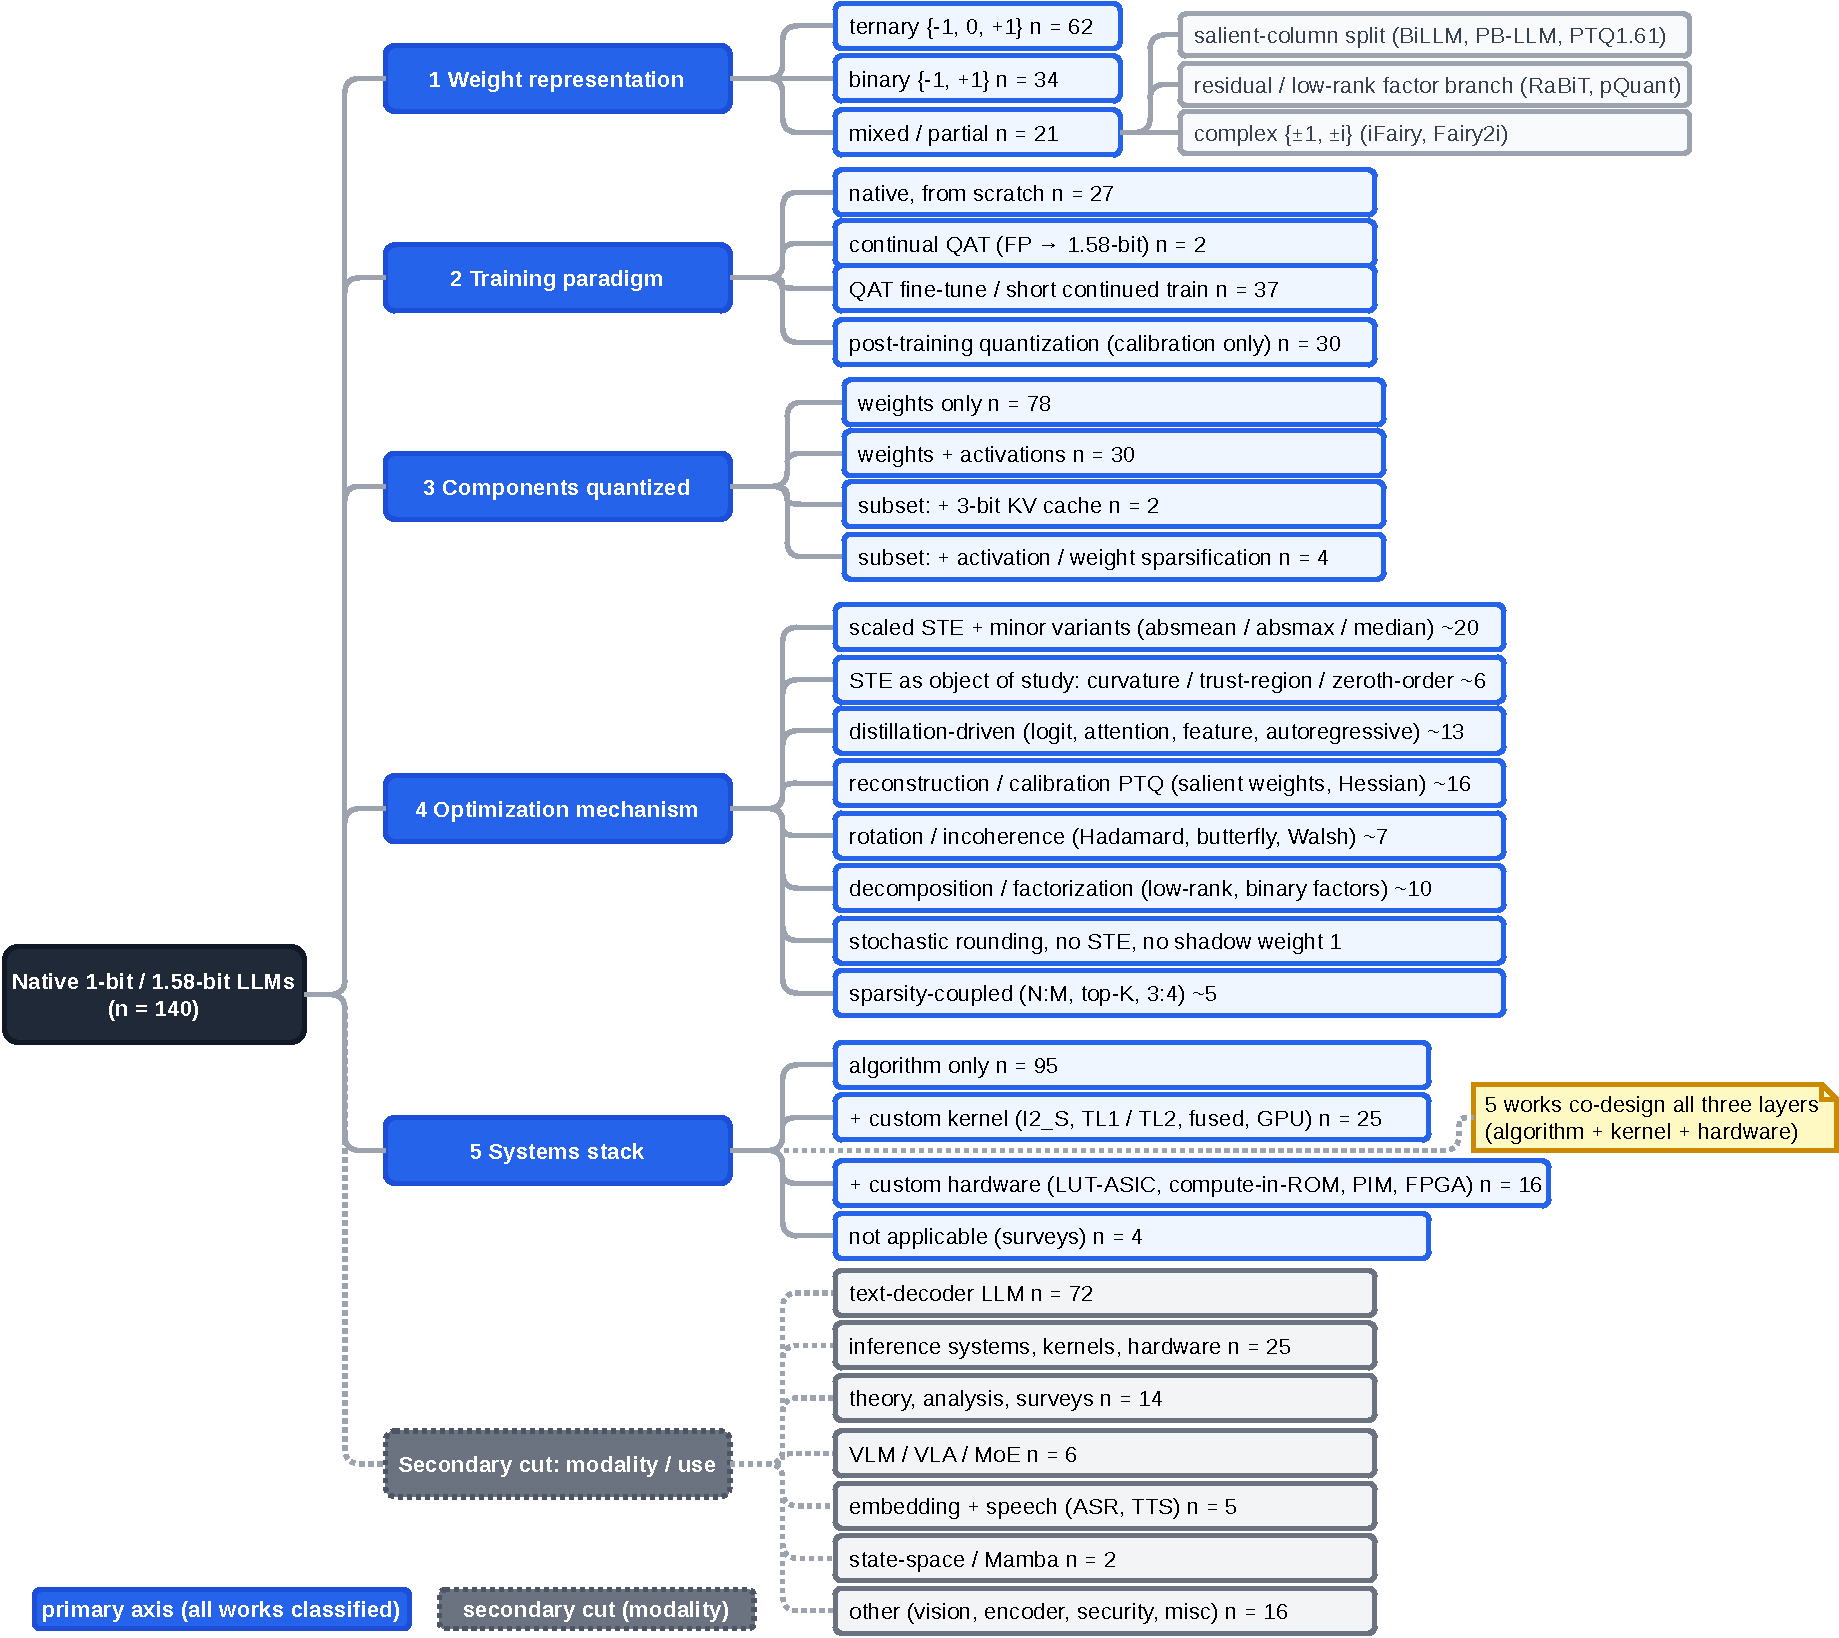
\includegraphics[width=\textwidth]{fig1-taxonomy.pdf}
\caption{Five-axis taxonomy of the surveyed corpus (135 in-window works plus five pre-2023 foundational works, listed in Table 1). Axes 1, 2, 3, and 5 partition all 140 works; axis 4 (optimization mechanism) is a non-exclusive tally and does not sum to 140. The modality cut at the bottom is a secondary partition.}
\label{fig:taxonomy}
\end{figure}


\begin{figure}[htbp]
\centering
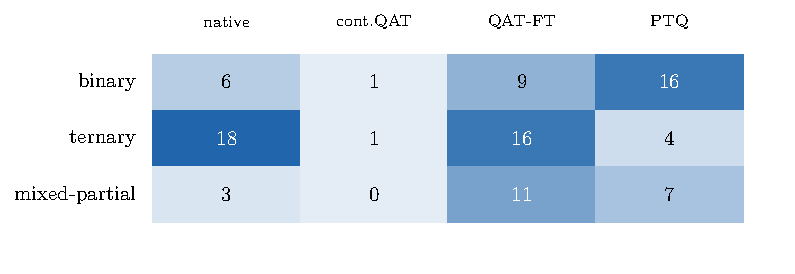
\includegraphics{fig-heatmap.pdf}
\caption{Weight representation against training paradigm, restricted to the three weight types and four paradigms that carry a training procedure (systems, analysis, and survey works are excluded). Native training concentrates on ternary (18 of 27 native works); post-training quantization concentrates on binary (16 of 27 PTQ works).}
\label{fig:heatmap}
\end{figure}


\begin{figure}[htbp]
\centering
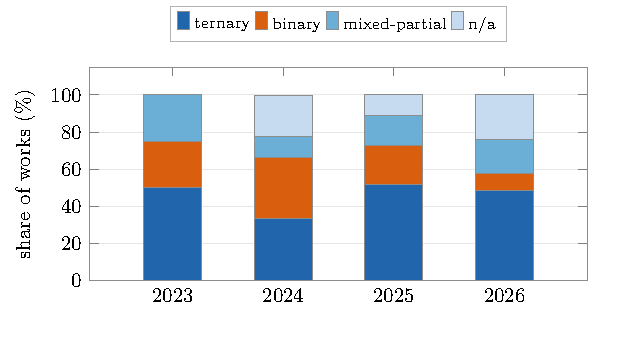
\includegraphics{fig-weightyear.pdf}
\caption{Weight-representation share by year, each bar normalized to 100\% of that year's works. Binary peaked at a third of new work in 2024 and fell to under a tenth by 2026; ternary stayed largest or second-largest throughout. 2023 (four works) and 2026 (partial year) should be read cautiously.}
\label{fig:weightyear}
\end{figure}

\begin{landscape}
\begingroup\footnotesize\setlength{\tabcolsep}{4pt}\hbadness=10000 \hfuzz=2pt \emergencystretch=3em
\begin{longtable}{p{3.2cm} p{1cm} p{1.9cm} p{2.2cm} p{2.2cm} p{1.3cm} p{2.2cm} p{2.1cm} p{2.5cm}}
\caption{Classification of the surveyed corpus on the taxonomy axes. Weight type, training paradigm, and quantized components each partition the corpus; their counts sum to 140. \emph{Evidence basis} gives venue (\emph{preprint} if not peer reviewed) and independent-check status (\emph{ext.\ repro} for an external one); it is not a graded score. In the cells: \emph{n/a} = axis does not apply; \emph{NA} = not applicable (activation-bit/systems-layer); \emph{NR} = not reported; \emph{var} = a range rather than one value.}\label{tab:classification}\\
\toprule Reference & Year & Weight type & Training paradigm & Components quantized & Act. bits & Systems layer & Modality & Evidence basis \\ \midrule \endfirsthead
\toprule Reference & Year & Weight type & Training paradigm & Components quantized & Act. bits & Systems layer & Modality & Evidence basis \\ \midrule \endhead
\bottomrule \endfoot
\citet{Bengio2013-STE} & 2013 & binary & background & W & NA & algorithm & background & preprint \\
\citet{Courbariaux2015-BinaryConnect} & 2015 & binary & native-scratch & W & 32 & algorithm & vision & Neur\allowbreak{}IPS \\
\citet{Rastegari2016-XNORNet} & 2016 & binary & native-scratch & W+\allowbreak{}A & 1 & algo+\allowbreak{}kernel & vision & ECCV \\
\citet{Bai2021-BinaryBERT} & 2021 & binary & QAT-finetune & W+\allowbreak{}A & 8 & algorithm & text-encoder & ACL \\
\citet{Qin2022-BiBERT} & 2022 & binary & QAT-finetune & W+\allowbreak{}A+\allowbreak{}emb & 1 & algorithm & text-encoder & ICLR \\
\citet{Kim2023-TSLD} & 2023 & ternary & QAT-finetune & W & 16 & algorithm & text-decoder & Neur\allowbreak{}IPS \\
\citet{Wang2023-BitNet} & 2023 & binary & native-scratch & W+\allowbreak{}A & 8 & algo+\allowbreak{}kernel & text-decoder & JMLR \\
\citet{Shang2023-PBLLM} & 2023 & mixed-partial & PTQ & W & 16 & algorithm & text-decoder & ICLR \\
\citet{Ansar2024-BEExformer} & 2024 & binary & native-scratch & W & 16 & algorithm & text-encoder & IEEE-TSUSC \\
\citet{Chen2024-DBLLM} & 2024 & binary & PTQ & W & 16 & algorithm & text-decoder & ICLR \\
\citet{Chen2024-EfficientQAT} & 2024 & mixed-partial & QAT-finetune & W & 16 & algorithm & text-decoder & preprint \\
\citet{Daliri2024-Theory1bit} & 2024 & binary & analysis & W & NA & algorithm & theory & preprint \\
\citet{Dong2024-STBLLM} & 2024 & binary & PTQ & W & 16 & algo+\allowbreak{}kernel & text-decoder & ICLR25 \\
\citet{Du2024-BitDistiller} & 2024 & mixed-partial & QAT-finetune & W & 16 & algorithm & text-decoder & ACL \\
\citet{Das2024-GenBFA} & 2024 & n/\allowbreak{}a & analysis & W & 8 & NA & security & preprint \\
\citet{Gong2024-SurveyLowbit} & 2024 & n/\allowbreak{}a & survey & NA & NA & NA & survey & Neural-Networks \\
\citet{Huang2024-BiLLM} & 2024 & binary & PTQ & W & 16 & algorithm & text-decoder & ICML \\
\citet{Jo2024-BinaryMoS} & 2024 & binary & QAT-finetune & W & 16 & algorithm & text-decoder & Neur\allowbreak{}IPS \\
\citet{Kaushal2024-Spectra} & 2024 & ternary & native-scratch & W & 16 & algorithm & text-decoder & preprint +\allowbreak{} ext. repro \\
\citet{Zhao2024-DQT} & 2024 & ternary & native-scratch & W & 8 & algorithm & text-decoder & ACML \\
\citet{Kumar2024-ScalingLawsPrecision} & 2024 & n/\allowbreak{}a & analysis & W+\allowbreak{}A & var & algorithm & theory & ICLR25 \\
\citet{Li2024-ARBLLM} & 2024 & binary & PTQ & W & 16 & algorithm & text-decoder & ICLR25 \\
\citet{Ma2024-BitNetB158} & 2024 & ternary & native-scratch & W+\allowbreak{}A & 8 & algo+\allowbreak{}kernel+\allowbreak{}hw & text-decoder & preprint +\allowbreak{} ext. repro \\
\citet{Ma2024-FBILLM} & 2024 & binary & native-scratch & W & 16 & algorithm & text-decoder & preprint \\
\citet{Malekar2024-MatmulOrNot} & 2024 & n/\allowbreak{}a & analysis & NA & NA & hardware & analysis & preprint \\
\citet{Malinovskii2024-PVTuning} & 2024 & mixed-partial & QAT-finetune & W & 16 & algorithm & text-decoder & Neur\allowbreak{}IPS(oral) \\
\citet{Nielsen2024-Reloaded} & 2024 & ternary & native-scratch & W+\allowbreak{}A & 8 & algorithm & small-LM/\allowbreak{}vision & preprint \\
\citet{Nielsen2024-WhenEnough} & 2024 & ternary & native-scratch & W & 16 & algorithm & MLP/\allowbreak{}GNN/\allowbreak{}encoder & preprint \\
\citet{Ouyang2024-QiDScaling} & 2024 & n/\allowbreak{}a & analysis & W & var & algorithm & theory & preprint \\
\citet{Sundaram2024-LLaVaOLMoBitnet} & 2024 & ternary & native-scratch & W+\allowbreak{}A & 8 & algorithm & VLM & preprint \\
\citet{Tang2024-BiMamba} & 2024 & binary & native-scratch & W & 16 & algorithm & SSM & TMLR \\
\citet{Wang2024-1bitAIInfra} & 2024 & ternary & systems & NA & NA & kernel+\allowbreak{}hw & systems & preprint \\
\citet{Wang2024-BitNetA48} & 2024 & ternary & native-scratch & W+\allowbreak{}A+\allowbreak{}KV+\allowbreak{}sparsify & 4 & algo+\allowbreak{}kernel & text-decoder & preprint \\
\citet{Wang2024-QSparse} & 2024 & ternary & native-scratch & A-sparsify & 8 & algorithm & text-decoder & preprint \\
\citet{Xu2024-OneBit} & 2024 & binary & QAT-finetune & W & 16 & algorithm & text-decoder & Neur\allowbreak{}IPS \\
\citet{Zhu2024-MatmulFree} & 2024 & ternary & native-scratch & W+\allowbreak{}A & 8 & algo+\allowbreak{}kernel+\allowbreak{}hw & text-decoder & preprint \\
\citet{Dehghankar2024-EfficientMatmul} & 2024 & n/\allowbreak{}a & systems & W & NA & algorithm & systems & ICML25 \\
\citet{Chen2024-TernaryEmbedding} & 2024 & ternary & QAT-finetune & W & 16 & algorithm & embedding & preprint \\
\citet{Fan2024-ResilientEfficient} & 2024 & n/\allowbreak{}a & analysis & NA & NA & NA & analysis-security & preprint \\
\citet{Kawamura2025-BitTTS} & 2025 & ternary & QAT-finetune & W & 16 & algorithm & TTS & Interspeech \\
\citet{Ye2025-DBellQuant} & 2025 & binary & PTQ & W+\allowbreak{}A & 6 & algorithm & text-decoder & preprint \\
\citet{Hoang2025-OutputAlign1bit} & 2025 & binary & PTQ & W & 16 & algorithm & text-decoder & preprint \\
\citet{Huang2025-Tequila} & 2025 & ternary & QAT-finetune & W & 16 & algorithm & text-decoder & preprint \\
\citet{Vaidhya2025-Spectra11} & 2025 & ternary & native-scratch & W & 16 & algo+\allowbreak{}kernel & text-decoder & preprint +\allowbreak{} ext. repro \\
\citet{Ardakani2025-LLMPi} & 2025 & ternary & systems & W+\allowbreak{}A & 8 & kernel+\allowbreak{}hw & edge-systems & CVPRW \\
\citet{Lee2025-LittleBit} & 2025 & binary & QAT-finetune & W & 16 & algorithm & text-decoder & Neur\allowbreak{}IPS \\
\citet{Liu2025-SurveyBNNLLM} & 2025 & n/\allowbreak{}a & survey & NA & NA & NA & survey & preprint \\
\citet{Ma2025-BitNet2B4T} & 2025 & ternary & native-scratch & W+\allowbreak{}A & 8 & algo+\allowbreak{}kernel+\allowbreak{}hw & text-decoder & preprint +\allowbreak{} Sec.10 \\
\citet{Wang2025-MoTE} & 2025 & ternary & native-scratch & W-experts & 16 & algorithm & VLM/\allowbreak{}Mo\allowbreak{}E & preprint \\
\citet{Nielsen2025-ContinualQAT} & 2025 & ternary & continual-QAT & W & 16 & algorithm & text-decoder & preprint \\
\citet{Yan2025-PT2LLM} & 2025 & ternary & PTQ & W & 16 & algorithm & text-decoder & ICLR26 \\
\citet{Xiao2025-PTQTP} & 2025 & ternary & PTQ & W & 16 & algorithm & text-decoder & preprint \\
\citet{Liu2025-ParetoQ} & 2025 & mixed-partial & QAT-finetune & W & 16 & algorithm & theory/\allowbreak{}text-decoder & Neur\allowbreak{}IPS +\allowbreak{} ext. repro \\
\citet{Panferov2025-QuEST} & 2025 & binary & QAT-finetune & W+\allowbreak{}A & 1 & algo+\allowbreak{}kernel & text-decoder & preprint \\
\citet{Oh2025-TSAR} & 2025 & ternary & systems & NA & NA & kernel+\allowbreak{}hw & systems & DATE26 \\
\citet{Tabesh2025-CAGE} & 2025 & mixed-partial & QAT-finetune & W+\allowbreak{}A & 3 & algorithm & text-decoder & MLSys26 \\
\citet{Xu2025-TeLLMe} & 2025 & ternary & systems & NA & NA & hardware & systems & preprint \\
\citet{Chen2025-TerEffic} & 2025 & ternary & systems & NA & NA & hardware & systems & preprint \\
\citet{Tu2025-Rethink1bitOpt} & 2025 & binary & continual-QAT & W & 16 & algorithm & text-decoder & preprint \\
\citet{Wang2025-BitNetJMLR} & 2025 & mixed-partial & native-scratch & W+\allowbreak{}A & 8 & algo+\allowbreak{}kernel & text-decoder & JMLR \\
\citet{Wang2025-BitNetCPP} & 2025 & ternary & systems & NA & NA & kernel & systems & ACL \\
\citet{Wang2025-BitNetV2} & 2025 & ternary & native-scratch & W+\allowbreak{}A+\allowbreak{}KV & 4 & algo+\allowbreak{}kernel & text-decoder & preprint \\
\citet{Wang2025-BitVLA} & 2025 & ternary & native-scratch & W+\allowbreak{}A & 8 & algorithm & VLA & preprint \\
\citet{Anon2025-BinaryWA-PTQ} & 2025 & binary & PTQ & W+\allowbreak{}A & 1 & algorithm & text-decoder & preprint \\
\citet{Anon2025-DoubleBinaryFactorization} & 2025 & binary & PTQ & W & 16 & algorithm & text-decoder & TMLR \\
\citet{Wu2025-BitNetDistillation} & 2025 & ternary & QAT-finetune & W+\allowbreak{}A & 8 & algorithm & text-decoder & preprint \\
\citet{Zhang2025-BitROM} & 2025 & ternary & systems & NA & NA & hardware & systems & ASP-DAC \\
\citet{Gu2025-BTCLLM} & 2025 & binary & PTQ & W & 16 & algorithm & text-decoder & preprint \\
\citet{Anon2025-CPUvsGPU} & 2025 & ternary & systems & NA & NA & hardware & systems & preprint \\
\citet{Anon2025-CompressionScalingLaws} & 2025 & n/\allowbreak{}a & analysis & W & var & algorithm & theory & preprint \\
\citet{Chen2025-HBLLM} & 2025 & binary & PTQ & W & 16 & algorithm & text-decoder & preprint \\
\citet{Anon2025-STE-ZerothOrder} & 2025 & mixed-partial & QAT-finetune & W & 16 & algorithm & text-decoder & Neur\allowbreak{}IPS \\
\citet{Chen2025-LoTAQAF} & 2025 & ternary & QAT-finetune & W & 16 & algorithm & text-decoder & preprint \\
\citet{Hao2025-LowPrecTrainingSurvey} & 2025 & n/\allowbreak{}a & survey & W+\allowbreak{}A & var & algorithm & survey & IEEE-TPAMI \\
\citet{Anon2025-MultiBoolean} & 2025 & binary & PTQ & W & 16 & algorithm & text-decoder & ICLR \\
\citet{Malekar2025-PIMLLM} & 2025 & ternary & systems & NA & NA & hardware & systems & preprint \\
\citet{Anon2025-ProgBinPruning} & 2025 & binary & PTQ & W & 16 & algo+\allowbreak{}kernel & text-decoder & preprint \\
\citet{Zhao2025-PTQ161} & 2025 & mixed-partial & PTQ & W & 16 & algorithm & text-decoder & ACL \\
\citet{Xia2025-SDQLLM} & 2025 & binary & PTQ & W & 16 & algorithm & text-decoder & ECAI \\
\citet{Anon2025-TENET} & 2025 & ternary & systems & NA & NA & hardware & systems & preprint \\
\citet{Anon2025-VLMTernarization} & 2025 & ternary & QAT-finetune & W & 16 & algorithm & VLM & preprint \\
\citet{Anon2025-OneBitASR} & 2025 & binary & QAT-finetune & W & 16 & algorithm & ASR & Interspeech \\
\citet{Connor2025-UltraQuantisation} & 2025 & ternary & QAT-finetune & W & 16 & algorithm & embedding & preprint \\
\citet{Huang2026-Sherry} & 2026 & ternary & QAT-finetune & W & 16 & algo+\allowbreak{}kernel & text-decoder & preprint \\
\citet{Li2026-BitNetTextEmbeddings} & 2026 & ternary & native-scratch & W & 8 & algorithm & embedding & preprint \\
\citet{Anon2026-Litespark} & 2026 & ternary & systems & NA & NA & kernel & systems & preprint \\
\citet{Anon2026-NativeTernary} & 2026 & ternary & systems & W & NA & algorithm & storage & preprint \\
\citet{Song2026-LBLLM} & 2026 & mixed-partial & PTQ & W+\allowbreak{}A & 4 & algorithm & text-decoder & preprint \\
\citet{Nargund2026-TernaryLM} & 2026 & ternary & native-scratch & W & 16 & algorithm & text-decoder & preprint \\
\citet{Zhang2026-SparseBitNet} & 2026 & ternary & native-scratch & W+\allowbreak{}sparsify & 8 & algo+\allowbreak{}kernel+\allowbreak{}hw & text-decoder & preprint \\
\citet{Zhao2026-TWLA} & 2026 & ternary & PTQ & W+\allowbreak{}A & 4 & algorithm & text-decoder & preprint \\
\citet{Zuo2026-FairyFuse} & 2026 & ternary & systems & NA & NA & kernel & systems & preprint \\
\citet{Wang2026-CATQ} & 2026 & ternary & PTQ & W & 16 & algorithm & text-decoder & preprint \\
\citet{Anon2026-EveryBitCounts} & 2026 & n/\allowbreak{}a & analysis & W & var & algorithm & theory & preprint \\
\citet{Anon2026-ExpressivePowerWQ} & 2026 & n/\allowbreak{}a & analysis & W & var & algorithm & theory & preprint \\
\citet{Wang2026-HESTIA} & 2026 & mixed-partial & QAT-finetune & W & 16 & algorithm & text-decoder & preprint \\
\citet{Anon2026-HGF} & 2026 & ternary & native-scratch & W & 16 & algorithm & text-decoder & preprint \\
\citet{Chong2026-NanoQuant} & 2026 & binary & PTQ & W & 16 & algorithm & text-decoder & preprint \\
\citet{You2026-RaBiT} & 2026 & binary & QAT-finetune & W & 16 & algorithm & text-decoder & preprint \\
\citet{Zagitov2026-HARP} & 2026 & n/\allowbreak{}a & PTQ & W+\allowbreak{}A & 2 & algorithm & text-decoder & preprint \\
\citet{Pavlov2026-InfluenceRotations} & 2026 & n/\allowbreak{}a & PTQ & W & 2 & algorithm & text-decoder & preprint \\
\citet{Zhang2026-pQuant} & 2026 & mixed-partial & QAT-finetune & W & 16 & algorithm & text-decoder & preprint \\
\citet{Wang2026-LCQAT} & 2026 & mixed-partial & QAT-finetune & W & 16 & algorithm & text-decoder & ICML \\
\citet{Alimaskina2026-ExtremeReasoning} & 2026 & n/\allowbreak{}a & analysis & W & 2 & algorithm & reasoning & preprint \\
\citet{Zhao2026-BWLA} & 2026 & binary & PTQ & W+\allowbreak{}A & 6 & algorithm & text-decoder & preprint \\
\citet{Xu2026-FittingNotEnough} & 2026 & n/\allowbreak{}a & analysis & W & var & algorithm & theory & preprint \\
\citet{Wang2025-Fairy2i} & 2025 & mixed-partial & PTQ & W & 16 & algorithm & text-decoder & preprint \\
\citet{Maskey2026-1BitWonder} & 2026 & n/\allowbreak{}a & QAT-finetune & W & 16 & algorithm & text-decoder & preprint \\
\citet{Li2025-ICQuant} & 2025 & n/\allowbreak{}a & PTQ & W & 16 & algorithm & text-decoder & COLM \\
\citet{Wang2025-TZLLM} & 2025 & n/\allowbreak{}a & systems & NA & NA & hardware & security & Euro\allowbreak{}Sys \\
\citet{Shan2025-Platinum} & 2025 & ternary & systems & NA & NA & hardware & systems & ASP-DAC \\
\citet{Li2025-VecLUT} & 2025 & ternary & systems & NA & NA & kernel & systems & Mobi\allowbreak{}Sys \\
\citet{Guan2026-TOM} & 2026 & ternary & systems & NA & NA & hardware & systems & preprint \\
\citet{Qiao2025-TeLLMev2} & 2025 & ternary & systems & NA & NA & hardware & systems & preprint \\
\citet{Jorgensen2025-ResourceEfficientLMs} & 2025 & n/\allowbreak{}a & survey & NA & NA & algorithm & survey & preprint \\
\citet{Aman2025-BitMar} & 2025 & mixed-partial & native-scratch & W & 16 & algorithm & VLM & preprint \\
\citet{Chen2025-R2Q} & 2025 & mixed-partial & QAT-finetune & W & 16 & algorithm & text-decoder & preprint \\
\citet{Zhang2026-EdgeRazor} & 2026 & mixed-partial & QAT-finetune & W+\allowbreak{}A & 16 & algorithm & text-decoder & preprint \\
\citet{Dehghankar2026-RSRcore} & 2026 & n/\allowbreak{}a & systems & NA & NA & kernel & systems & preprint \\
\citet{Grainge2025-TeTRAVPR} & 2025 & ternary & QAT-finetune & W & 16 & algorithm & vision & IEEE-RAL \\
\citet{Wang2025-iFairy} & 2025 & mixed-partial & native-scratch & W & 16 & algorithm & text-decoder & preprint \\
\citet{Ganesaraja2026-TernaryMamba} & 2026 & ternary & QAT-finetune & W & 16 & algorithm & SSM & preprint \\
\citet{Zhang2025-TernaryCLIP} & 2025 & ternary & QAT-finetune & W & 16 & algorithm & VLM & preprint \\
\citet{Steinmetz2025-ExtraRMSNorm} & 2025 & ternary & QAT-finetune & W & 16 & algorithm & text-decoder & preprint \\
\citet{Ortega2024-PIMAI} & 2024 & n/\allowbreak{}a & systems & NA & NA & hardware & systems & preprint \\
\citet{Liu2023-BinTernNLG} & 2023 & ternary & QAT-finetune & W+\allowbreak{}A & 8 & algorithm & text-seq2seq & preprint \\
\citet{Wei2024-TMAC} & 2024 & ternary & systems & NA & NA & kernel & systems & preprint \\
\citet{Ji2024-BMTBAT} & 2024 & binary & QAT-finetune & W+\allowbreak{}A & NR & algo+\allowbreak{}kernel+\allowbreak{}hw & text-decoder & preprint \\
\citet{Xu2024-CRVQ} & 2024 & mixed-partial & PTQ & W & 16 & algorithm & text-decoder & preprint \\
\citet{Edalati2024-OAC} & 2024 & binary & PTQ & W & 16 & algorithm & text-decoder & preprint \\
\citet{Malhotra2025-ReTern} & 2025 & ternary & systems & W+\allowbreak{}A & 8 & hardware & systems & preprint \\
\citet{Xiao2025-LieQ} & 2025 & mixed-partial & PTQ & W & 16 & algorithm & text-decoder & preprint \\
\citet{Georganas2025-UltraLowBitKernels} & 2025 & n/\allowbreak{}a & systems & NA & NA & kernel & systems & preprint \\
\citet{Qi2025-DeltaLLM} & 2025 & ternary & systems & A-sparsify & 8 & algorithm & text-decoder & preprint \\
\citet{Zhang2025-PDSwap} & 2025 & ternary & systems & NA & NA & hardware & systems & preprint \\
\citet{Sajid2026-BitRL} & 2026 & ternary & QAT-finetune & W+\allowbreak{}A & 8 & algorithm & RL & preprint \\
\citet{Geens2026-LUTAccelDesign} & 2026 & ternary & systems & NA & NA & hardware & systems & preprint \\
\citet{Lin2026-VitaLLM} & 2026 & ternary & systems & NA & NA & hardware & systems & preprint \\
\citet{Kang2026-BitTP} & 2026 & ternary & QAT-finetune & W & 16 & algorithm & robotics & preprint \\
\citet{Abdalla2026-SAGEPTQ} & 2026 & mixed-partial & PTQ & W & 16 & algorithm & text-decoder & preprint \\
\end{longtable}
\endgroup
\end{landscape}


%% ===== 05-architecture
\section{Architectural Design}

\subsection{The BitLinear primitive}

The standard native 1-bit LLM is built from a single substitution: the standard linear
layer is
replaced by a \texttt{BitLinear} layer that normalizes its input, quantizes the weight to a
low-bit code with a shared scale, quantizes the activation, and back-propagates through
both quantizers with a straight-through estimator \cite{Wang2023-BitNet},
\cite{Wang2025-BitNetJMLR}. In the original BitNet, the weight rule is a sign function
applied after subtracting the mean and dividing by the mean absolute value, and the
activation rule is per-token absolute-max quantization to INT8, offset for
non-linearities that produce non-negative outputs. BitNet b1.58 changes the weight rule
to an absolute-mean ternary quantizer: it divides by the mean absolute value, rounds to
the nearest of \{-1,0,+1\}, and clamps. This yields the \{-1,0,+1\} value set and drives
roughly half of the weights to zero \cite{Ma2024-BitNetB158}. Small-model studies report that
using the median in place of the mean in the scale makes the quantizer less sensitive
to a few large weights and can improve accuracy at very small scales
\cite{Nielsen2024-Reloaded}.

A recurring architectural detail is the placement of normalization. \texttt{BitLinear} applies
its normalization, LayerNorm in BitNet and SubLN in later variants, before quantization,
so that the quantizer sees a controlled input distribution. Several works find that an
additional RMSNorm inserted at the layer boundary stabilizes the transition to 1.58-bit
weights during fine-tuning \cite{Steinmetz2025-ExtraRMSNorm}, and BitNet Distillation
combines SubLN with a short continued-pretraining phase before task distillation
\cite{Wu2025-BitNetDistillation}.

\subsection{Ternary versus binary in practice}

The move from binary to ternary is the single largest architectural lever in the native
setting. Binary from-scratch training is possible: FBI-LLM demonstrates a fully binary
LLM that matches half precision by relying heavily on an autoregressive distillation
loss \cite{Ma2024-FBILLM}, and QuEST reaches stable one-bit weights and activations with a
trust-gradient estimator and Hadamard-normalized fitting \cite{Panferov2025-QuEST}. In each
case, however, more machinery, such as distillation, careful initialization, or a better
gradient estimator, is needed to reach the loss that ternary attains directly. The zero
state of ternary weights doubles as sparsity, unstructured until a method imposes a
pattern on it (Section 5.5), which is why ternary models
compose naturally with N:M sparse tensor cores \cite{Zhang2026-SparseBitNet} and with packing
schemes that store four ternary weights in five bits \cite{Huang2026-Sherry} or approach the
1.6-bit information bound \cite{Vaidhya2025-Spectra11}.

\subsection{Activation quantization}

Once weights occupy roughly one bit, activation precision becomes the binding
constraint. Most native models keep activations at INT8 \cite{Ma2024-BitNetB158},
\cite{Ma2025-BitNet2B4T}. Two routes go lower. BitNet a4.8 uses a hybrid scheme: INT4
activations for the inputs to attention and the feed-forward network, but the
outlier-heavy intermediate states, namely the attention output and the feed-forward
down-projection input, are first sparsified with a top-K mask and then quantized to
INT8. The effective configuration is W1.58A4 with only 55\% of parameters active and a
three-bit KV cache, and the feed-forward network uses a squared-ReLU gate that produces
about 80\% activation sparsity \cite{Wang2024-BitNetA48}. BitNet v2 instead rotates: an
online Hadamard transform inside a modified \texttt{H-BitLinear} layer spreads outlier energy
across coordinates so that a plain INT4 or FP4 quantizer suffices for all activations
natively \cite{Wang2025-BitNetV2}. Post-training work has converged on the same rotation
idea with learned or data-adaptive transforms, including butterfly-structured orthogonal
processors \cite{Zagitov2026-HARP}, Kronecker-structured rotations \cite{Zhao2026-TWLA},
orthogonal-Kronecker transforms with proximal-SVD refinement that reach W1A6
\cite{Zhao2026-BWLA}, and influence-weighted Walsh rescaling \cite{Pavlov2026-InfluenceRotations}.
Fig. \ref{fig:datapath} draws the three datapaths side by side: the plain \texttt{BitLinear} layer, the
Hadamard-rotated \texttt{H-BitLinear} layer, and the hybrid split-and-sparsify path of BitNet
a4.8. The current practical floor for activations alongside roughly one-bit weights is
four bits natively; post-training quantization mostly lands at six bits, though TWLA
reports four through the same Kronecker-rotation family on a single preprint benchmark
\cite{Zhao2026-TWLA}, not yet corroborated elsewhere. Whether A2 is reachable at all is an
open question (Section 11).

\subsection{KV cache}

The KV cache dominates memory for long contexts. BitNet a4.8 and BitNet v2 both quantize
it to three bits with no reported accuracy cost \cite{Wang2024-BitNetA48},
\cite{Wang2025-BitNetV2}. Dedicated KV-cache quantization for ternary models, using
signed-digit lookup schemes and sub-one-bit residual quantization of keys and values,
is an active topic in 2026, although much of it falls after the cutoff of this survey.

\subsection{Beyond the dense decoder}

For mixture-of-experts models, MoTE trains more low-precision experts rather than fewer
high-precision ones. Starting from a dense checkpoint, it up-cycles the feed-forward
network into one shared full-precision expert and many ternary routed experts, keeping
the active-parameter count fixed while eliminating the memory overhead of a
full-precision expert pool \cite{Wang2025-MoTE}. Q-Sparse shows that full activation sparsity
composes with both BitNet b1.58 and mixture-of-experts, and derives an inference-optimal
scaling law for the combination \cite{Wang2024-QSparse}.

For state-space models, Bi-Mamba binarizes a Mamba model from scratch with an
autoregressive distillation loss and matches half precision at up to 2.7B parameters,
opening a low-bit path for linear-complexity architectures \cite{Tang2024-BiMamba}; Ternary
Mamba applies grouped quantization-aware training at W1.58A16
\cite{Ganesaraja2026-TernaryMamba}.

For sub-1.58-bit representations, Sparse-BitNet observes that ternary models tolerate
N:M structured sparsity far better than full-precision models, since their weights are
already about 42\% zero, and applies dynamic N:M sparsification jointly with 1.58-bit
quantization, backed by custom sparse tensor-core kernels \cite{Zhang2026-SparseBitNet}.
Sherry regularizes this to a 3:4 pattern that packs to a power-of-two-aligned 1.25 bits
\cite{Huang2026-Sherry}. Structural binarization below one bit \cite{Dong2024-STBLLM} and
latent-factorization schemes that reach about 0.1 bits per weight \cite{Lee2025-LittleBit}
are the current extreme.

\subsection{One-bit attention and matrix-multiplication-free designs}

BitNet quantizes only the projection layers and leaves the attention score computation
in higher precision, which caps the achievable speedup \cite{Malekar2024-MatmulOrNot}.
MatMul-free LM removes the remaining matrix multiplications by replacing self-attention
with a gated linear-attention recurrence over ternary \texttt{BitLinear} layers, so that the
whole model consists of additions and element-wise operations; it matches an optimized
Transformer baseline up to 2.7B parameters and has been mapped to FPGA and neuromorphic
hardware \cite{Zhu2024-MatmulFree}. One-bit query-key attention and fully additive
accumulation through complex $\{\pm 1, \pm i\}$ codebooks \cite{Wang2025-iFairy},
\cite{Wang2025-Fairy2i} are further points on this line.



\begin{figure}[htbp]
\centering
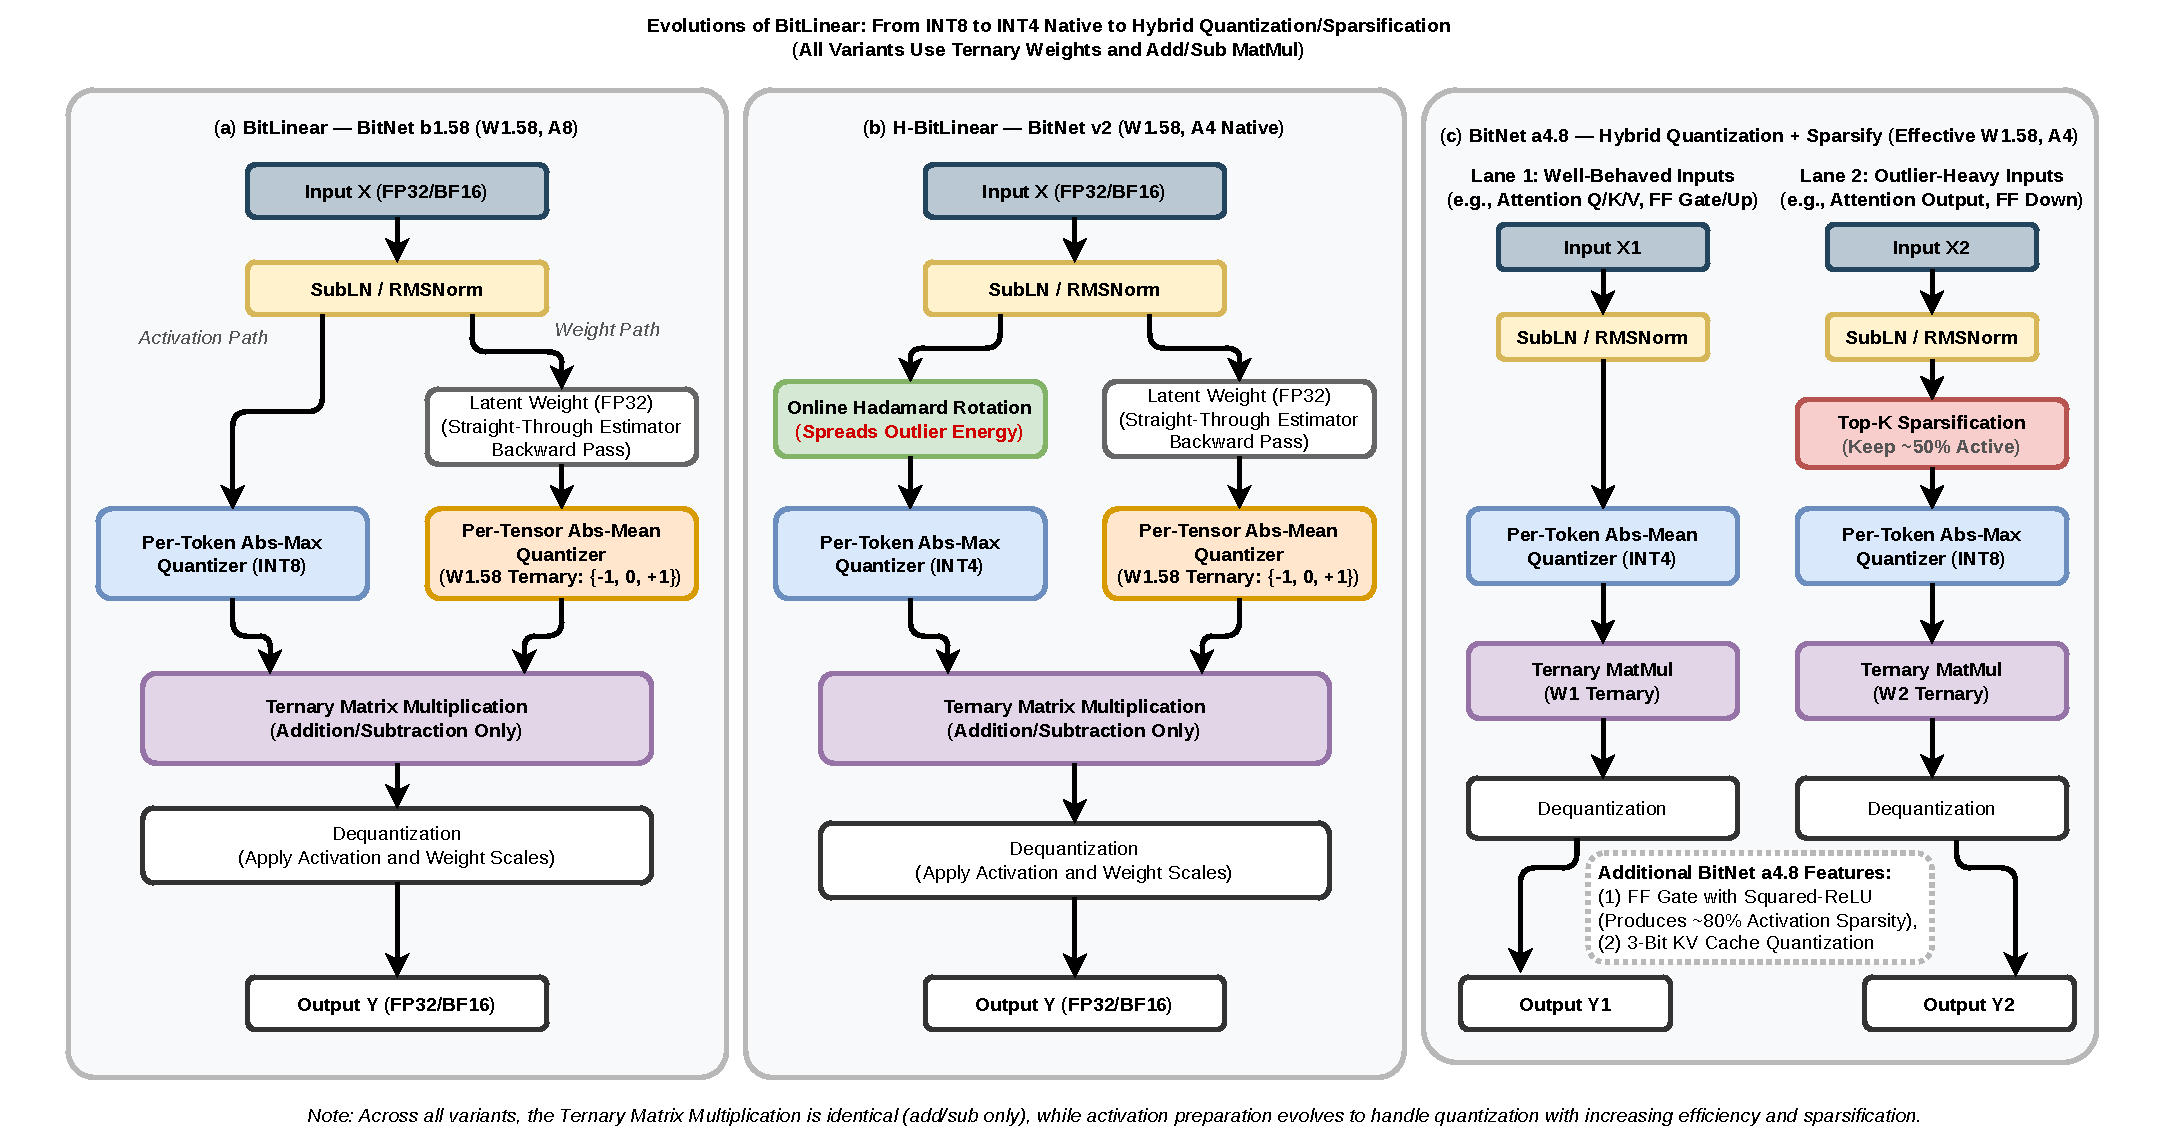
\includegraphics[width=\textwidth]{fig-datapath.pdf}
\caption{Three \texttt{BitLinear} datapath variants on a common template. Blue is the activation quantizer, orange the weight quantizer, and purple the ternary matrix multiplication, identical across all three. (a) BitLinear (BitNet b1.58): INT8 activations. (b) H-BitLinear (BitNet v2): an online Hadamard rotation (green) enables INT4 activations. (c) BitNet a4.8: well-behaved inputs go directly to INT4; outlier-heavy inputs are top-K sparsified (red) then quantized to INT8. All three retain a full-precision latent weight trained with a straight-through estimator.}
\label{fig:datapath}
\end{figure}



%% ===== 06-training
\section{Training Methodology and Theory}

\subsection{The native training loop}

Native 1-bit training keeps a full-precision shadow weight in the optimizer and derives
the quantized weight from it on the fly in every forward pass. The forward pass uses
the quantized weight; the backward pass computes gradients with respect to the
quantized weight and applies them to the shadow weight through the straight-through
estimator, usually clipped to the active range of the quantizer
\cite{Wang2023-BitNet,Ma2024-BitNetB158}. At the end of
training, the shadow weights are quantized once and discarded, leaving a model that
stores about 1.58 bits per weight and, with an appropriate kernel, replaces its matrix
multiplications with integer additions. The cost of this scheme is training-time memory:
the shadow weights and their optimizer state are full precision, adding the memory
footprint of a full-precision copy of the model on top of the quantized forward pass,
and the compression saving is realized entirely at inference time. Direct Quantized Training questions the shadow copy itself,
keeping only low-precision weights and using stochastic rounding to carry sub-quantum
information between steps; it reports that ternary-only training is feasible and that
widening to eight-bit weights matches BitNet b1.58 at reduced training memory
\cite{Zhao2024-DQT}.

\subsection{Recipes}

The published recipes share a common shape. There is a two-stage schedule for the
learning rate and weight decay, with higher values early, when the quantized landscape
is rough, and lower values later; a warmup on the quantization strength; and, for
instruction-tuned models, a standard supervised fine-tuning stage followed by direct
preference optimization, applied while the weights remain ternary \cite{Ma2025-BitNet2B4T}.
Data scale matters more than parameter scale for ternary models: the Spectra suites
find that TriLM performance improves faster with training tokens than with parameters,
and Spectra 1.1 trains to 1.2T tokens on that basis \cite{Kaushal2024-Spectra},
\cite{Vaidhya2025-Spectra11}. Continual schemes trade a small amount of accuracy for a large
training saving by running most of pre-training in full precision and only the final
phase in 1.58-bit; the loss spike at the transition is reduced by retaining the
optimizer state across the switch and by phasing in the quantization strength gradually
\cite{Nielsen2025-ContinualQAT,Tu2025-Rethink1bitOpt}.

\subsection{The straight-through estimator and its alternatives}

The straight-through estimator is biased: the gradient it supplies is not the gradient
of the expected quantized loss, and the mismatch grows as the bit-width falls,
producing slow convergence and instability. Recent work treats the estimator as a
design object, along several lines.

The first line is curvature-aware estimation. CAGE frames quantization-aware training as
a multi-objective optimization that simultaneously minimizes the task loss and the
quantization error, derives a Pareto-optimality condition, and adds a curvature-
dependent correction term to the STE gradient, with a convergence proof in the smooth
non-convex setting; it matches the accuracy of a prior W4A4 method at W3A3
\cite{Tabesh2025-CAGE}.

The second line is trust-region estimation. QuEST fits the continuous weight and
activation distributions with a Hadamard normalization and an MSE-optimal grid, and then
uses a trust gradient that explicitly minimizes the distance between the quantized-state
gradient and the unknown true gradient; this is what allows it to train stably at
one-bit weights and activations \cite{Panferov2025-QuEST}.

The third line adds zeroth-order information: a finite-difference estimate of the true
gradient, added to the STE gradient, reduces its bias at low bit-width
\cite{Anon2025-STE-ZerothOrder}. A fourth line replaces the uniform quantizer with a
non-uniform one; a k-means codebook improves low-bit quantization-aware training by
placing levels where the weight mass is \cite{Maskey2026-1BitWonder}.

A final line moves beyond the STE for fine-tuning. PV-Tuning shows that the STE is
suboptimal for extreme fine-tuning specifically, and replaces it with a
representation-agnostic coordinate descent that alternates updates of the discrete
assignment and the continuous parameters, achieving the first Pareto-optimal 2-bit
Llama-2 \cite{Malinovskii2024-PVTuning}. LC-QAT makes vector-quantized training
differentiable by parameterizing each codeword as a linear map of a discrete vector,
which avoids the codebook lookup in the training forward pass \cite{Wang2026-LCQAT}.

\subsection{Distillation}

Distillation from a full-precision teacher is the most common way to close the last
accuracy gap. FBI-LLM trains a binary model from scratch with an autoregressive
distillation loss and finds that a pretrained initialization is not required
\cite{Ma2024-FBILLM}; Bi-Mamba does the same for state-space models \cite{Tang2024-BiMamba}.
BitDistiller pairs quantization-aware training with a confidence-aware
Kullback-Leibler objective in a self-distillation loop for sub-four-bit weights
\cite{Du2024-BitDistiller}; token-scaled logit distillation was the first method to bring
ternary quantization-aware training of large generative models to within one perplexity
point of the teacher \cite{Kim2023-TSLD}. BitNet Distillation adds SubLN, a short
continued-pretraining phase, and combined logit-and-attention distillation to convert a
full-precision LLM into a 1.58-bit task model \cite{Wu2025-BitNetDistillation}. LBLLM stages
the process into a post-training-quantization initialization, layer-wise weight
distillation, and finally learning of the activation scales \cite{Song2026-LBLLM}.

\subsection{Post-training routes toward one bit}

The post-training-quantization branch, 30 works on the training-paradigm axis of
Section 4.2, approaches one bit without gradient updates. The techniques cluster into a few families. The first is salient-
weight handling with binary residual approximation, as in the roughly 1.08 effective
bits of BiLLM \cite{Huang2024-BiLLM} and the partial binarization of PB-LLM
\cite{Shang2023-PBLLM}. The second is alternating refinement of the binarization parameters,
as in ARB-LLM, which was the first binary post-training method to beat a half-precision
model of equal size \cite{Li2024-ARBLLM}. The third is ternary-specific quantizers with
iterative grid fitting and column reordering \cite{Yan2025-PT2LLM,Xiao2025-PTQTP}. The
fourth is explicit outlier handling, whether by index coding at a 0.3-bit overhead
\cite{Li2025-ICQuant} or by learned distribution transforms \cite{Ye2025-DBellQuant},
\cite{Zhao2026-BWLA}. The fifth is output-alignment objectives that correct the error
accumulation and representation-space anisotropy from which naive output-matching
post-training quantization suffers in the one-bit regime \cite{Hoang2025-OutputAlign1bit}.

\subsection{Scaling laws at one bit}

Whether native 1.58-bit models genuinely match full precision, or only appear to do so
under limited training-token budgets, is the central empirical dispute in the field.
Precision-aware scaling laws model low-precision training as a reduction of the
effective parameter count and predict that post-training-quantization degradation
increases with pre-training data, eventually making additional data harmful for a model
that will be quantized \cite{Kumar2024-ScalingLawsPrecision}. The quantization-induced
degradation study reaches a compatible conclusion from more than 1,500 checkpoints:
degradation grows with the number of training tokens, so that projections to
100-trillion-token models are pessimistic for low-bit quantization
\cite{Ouyang2024-QiDScaling}. On the other side, the native ternary suites show TriLMs
overtaking quantized and full-precision models on a bits-for-bits basis beyond about 1B
parameters \cite{Kaushal2024-Spectra,Vaidhya2025-Spectra11}, and the unified 1-bit to
4-bit study of ParetoQ finds a learning transition between two and three bits, with
ternary, two-bit, and three-bit quantization sharing a size-accuracy frontier that
beats four-bit and binary \cite{Liu2025-ParetoQ}. A partial reconciliation is that the two
camps measure different quantities, namely post-training quantization of a fixed model
against training under the constraint, and that the crossover point, not its existence,
is what matters in practice. Theory is beginning to bear on this: a kernel-limit
analysis proves a scaling law for 1-bit networks \cite{Daliri2024-Theory1bit}, and
precision-expressivity trade-offs are being formalized for quantized transformers
\cite{Anon2026-EveryBitCounts,Anon2026-ExpressivePowerWQ}.

\subsection{Training stability and smoothness}

Beyond the loss value, extremely quantized models show a degradation of smoothness: a
rapid reduction in the number of plausible next tokens within a prediction
neighborhood, which sparsifies the decoding tree and hurts generation quality
independently of perplexity. A smoothness-preserving term added to either post-training
quantization or quantization-aware training recovers additional accuracy
\cite{Xu2026-FittingNotEnough}. Tequila identifies deadzone trapping, in which ternary
weights become stuck at the \{-1,0\} or \{0,+1\} boundary and receive only noise gradients,
and repurposes the trapped weights as dynamic biases so that they receive a meaningful
signal, at near-zero inference overhead \cite{Huang2025-Tequila}. HGF stabilizes 1.58-bit
training with a per-layer gated low-rank correction \cite{Anon2026-HGF}. These are early
steps toward the training stability that a native 1-bit model an order of magnitude
larger than today's 2B, 4T-token ceiling would require (Section 11).


%% ===== 07-systems
\section{Inference Systems and Hardware}

\subsection{The need for a software stack}

A ternary weight matrix stored at two bits already reduces memory traffic by roughly
eight times relative to BF16, but a naive kernel still dequantizes to floating point and
runs an ordinary matrix multiplication, capturing none of the arithmetic saving.
Realizing the add-and-subtract inner product requires either bit-serial computation or
lookup tables, and both need dedicated kernels. The dominant cost in ternary inference
is the mixed-precision matrix multiplication of ternary weights against INT8
activations, so this is what the kernels target \cite{Wang2025-BitNetCPP}.

\subsection{bitnet.cpp and CPU kernels}

bitnet.cpp is the reference CPU stack for BitNet b1.58 and ternary models
\cite{Wang2024-1bitAIInfra,Wang2025-BitNetCPP}. It provides two kernel families. The \texttt{I2\_S}
kernel packs ternary weights as two-bit integers with a shared scale and performs
lossless integer inference. The \texttt{TL1} and \texttt{TL2} kernels are ternary lookup tables: \texttt{TL1}
precomputes the products of a small block of ternary weights against the possible
activation values and indexes into them, and \texttt{TL2} refines the packing to reduce the
spatial footprint of the table. Reported speedups over an FP16 baseline are 2.37 to 6.17
times on x86 and 1.37 to 5.07 times on ARM, with energy reductions of 72\% to 82\% on
x86 and 55\% to 70\% on ARM, and the headline demonstration is a 100B-parameter BitNet
b1.58 model running at five to seven tokens per second, comparable to human reading
speed, on a single CPU \cite{Wang2024-1bitAIInfra}. A 2026 update adds parallel kernels with
configurable tiling for a further 1.15 to 2.1 times \cite{web-microsoftBitNet}. Independent
CPU frameworks pursue the same goal by different means: Litespark uses hand-tuned SIMD
code \cite{Anon2026-Litespark}, FairyFuse uses fused ternary kernels that avoid materializing
intermediates \cite{Zuo2026-FairyFuse}, T-SAR repurposes the SIMD register file for
in-register lookup-table generation with a small instruction-set change \cite{Oh2025-TSAR},
and RSR-core implements the Redundant Segment Reduction algorithm as production CPU and
CUDA kernels, with a reported 62-times CPU speedup on ternary LLMs
\cite{Dehghankar2026-RSRcore}. A more general theoretical result gives an
$O(n^2 / \log n)$ matrix-vector algorithm for binary and ternary matrices by
preprocessing the fixed weight matrix into an index \cite{Dehghankar2024-EfficientMatmul}.

\subsection{GPU}

GPUs are optimized for dense floating-point matrix multiplication, so ternary weights
initially offered little benefit on them. This has changed. An official GPU kernel for
BitNet shipped in 2025 \cite{web-microsoftBitNet}; the TriRun kernel of Spectra 1.1
accelerates end-to-end ternary inference by up to five times over a floating-point
baseline by packing two ternary weights per byte \cite{Vaidhya2025-Spectra11}; and QuEST
provides GPU kernels for its W1 through W4 models \cite{Panferov2025-QuEST}. The
matrix-multiplication-free design sidesteps the question altogether by removing the
operation that GPUs are built for \cite{Zhu2024-MatmulFree}.

\subsection{Custom accelerators}

Ternary weights change what the ideal processor looks like, and a first wave of designs
explores the space. Lookup-table ASICs precompute partial products and index into them.
Platinum uses offline-generated construction paths and adaptive bit-serial or
ternary-weight execution, reporting a 73-times speedup over a spiking baseline and a
2.15-times speedup over a 16-thread CPU implementation in under one square millimetre of
chip area \cite{Shan2025-Platinum}; TENET is a sparsity-aware, lookup-table-centric edge
architecture \cite{Anon2025-TENET}; and Vec-LUT vectorizes the table lookup for parallelism
\cite{Li2025-VecLUT}. Compute-in-ROM designs store the rarely updated ternary base model as
standard-cell logic, exploiting the zero state to eliminate area for zero-valued
weights, with an SRAM layer of low-rank adapters for on-device adaptation: BitROM
targets billion-parameter models \cite{Zhang2025-BitROM} and TOM reports 3,306 tokens per
second on a BitNet-2B model with dynamic power gating of inactive ROM banks
\cite{Guan2026-TOM}. Processing-in-memory designs \cite{Malekar2025-PIMLLM,Ortega2024-PIMAI}
and edge-FPGA accelerators with table-lookup matrix multiplication for both the prefill
and decode phases \cite{Xu2025-TeLLMe,Qiao2025-TeLLMev2,Chen2025-TerEffic} complete the
picture. The fault tolerance of compute-in-memory ternary LLMs, which can exploit the
natural redundancy of the zero state, is itself a research topic.

\subsection{Summary of the systems corpus}

Three observations stand out. First, the CPU story is mature: several independent
frameworks now beat FP16 by factors of two to six with lossless accuracy, and the claim
that a capable model can run without a GPU is genuine. Second, the GPU and custom-silicon
work is early: the accelerator papers report simulator or single-chip results rather
than shipping parts, and no commercial processor exposes a ternary
matrix-multiplication primitive. Third, only five works in the entire corpus co-design
across algorithm, kernel, and hardware (Fig. \ref{fig:systemsvenn}); the rest optimize one layer while assuming the
others. Closing that gap, by building an add-and-subtract matrix-multiplication unit
with a matching memory layout and instruction-set extension, co-designed with the
training recipe, is the clearest systems opportunity (Section 11). Section 10 reports
our own CPU measurements against the figures cited above.



\begin{figure}[htbp]
\centering
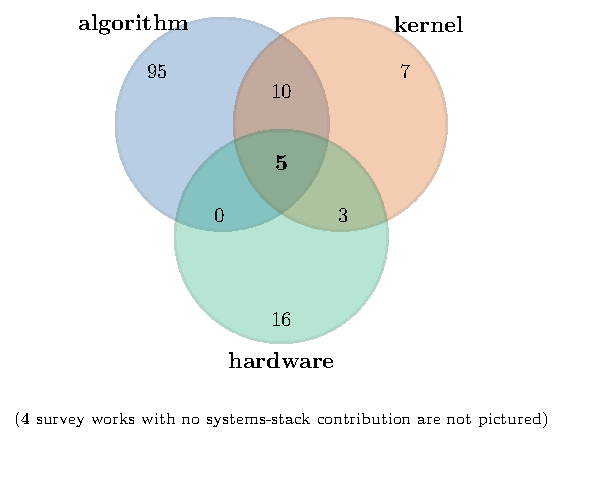
\includegraphics{fig-systemsvenn.pdf}
\caption{How far down the stack the corpus reaches: co-occurrence of algorithm, kernel, and hardware contributions; areas are illustrative, not proportional to count. Ninety-five works are algorithm only; only five co-design across all three layers.}
\label{fig:systemsvenn}
\end{figure}



%% ===== 07b-benchmarking
\section{Performance and Benchmarking}

\subsection{The comparison problem}

Results in this literature are difficult to align. Papers use different evaluation
harnesses and harness versions, different prompt formats and few-shot counts, and
different perplexity corpora, namely WikiText-2 against C4 validation; on the efficiency
side they differ in hardware, thread count, kernel, and baseline, whether FP16 against
INT8 or a general framework against a custom kernel. The reported number of bits per
weight also varies in what it includes (Section 2.1). We therefore report each claim in
the terms the source used, group claims by what is actually comparable, and flag cases
in which a direct comparison is not sound. Table 1 collects the headline figures; the
common-axis re-tabulation is Table 2; and our own independent measurements are in
Section 10.

\subsection{Perplexity and the parity claim}

The central claim of the native line is parity with a full-precision model of equal size
and training-token budget. BitNet b1.58 reports this from roughly 3B parameters: at 3B,
its WikiText-2 and C4 perplexity matches a reproduced FP16 LLaMA trained on the same
100B RedPajama tokens, its zero-shot average matches from the same scale, and the gap to
FP16 narrows as size grows to 7B \cite{Ma2024-BitNetB158,Wang2024-BitNetA48}. The Spectra
suites make the stronger claim that a ternary model can match a full-precision model of
equal parameter count: TriLM 3.9B matches FloatLM 3.9B across their benchmark set,
despite a higher perplexity and a size 5.9 times smaller in bits \cite{Kaushal2024-Spectra}.
Spectra 1.1 extends this to 1.2T tokens and finds that ternary models gain more from
data than from parameters \cite{Vaidhya2025-Spectra11}. The counter-evidence, discussed in
Section 6.6, is that post-training-quantization degradation grows with training tokens,
so these parity results, all measured at four trillion tokens or fewer, may not
extrapolate \cite{Kumar2024-ScalingLawsPrecision,Ouyang2024-QiDScaling}.

For post-training routes toward one bit, perplexity is the standard yardstick and the
progression is clear: BiLLM reached 8.41 on LLaMA2-70B at roughly 1.08 effective bits
\cite{Huang2024-BiLLM}; DB-LLM cut two-bit perplexity from 9.64 to 7.23 \cite{Chen2024-DBLLM}; the
rotation-and-column-bitmap variant of ARB-LLM was the first binary post-training method
to beat a half-precision model of the same size \cite{Li2024-ARBLLM}; and PTQTP and PT2-LLM
now bring training-free ternary within reach of 1.58-bit quantization-aware-training
accuracy in about an hour, rather than the 10 to 14 GPU-days that training requires
\cite{Xiao2025-PTQTP,Yan2025-PT2LLM}.

\subsection{Downstream benchmarks}

The common zero-shot suite is ARC-Easy, ARC-Challenge, HellaSwag, WinoGrande, PIQA,
OpenBookQA, and BoolQ, run through a standard harness and averaged; native-line papers
report this suite, while post-training-quantization papers more often report perplexity
plus a subset. For instruction-tuned models at the 2B scale, MMLU, GSM8K, and
HumanEval+ are added. BitNet b1.58 2B4T reports a zero-shot average of 54.19 against
55.23 for a full-precision Qwen2.5-1.5B, with the 1-bit model ahead on GSM8K
(58.38 against 56.79, a lead Section 10.3 reproduces) and ARC-Challenge (49.91) and behind
on MMLU (53.17 against 60.25, a deficit Section 10.3 also reproduces), and ahead of an
INT4-AWQ Qwen2.5-1.5B on the average \cite{Ma2025-BitNet2B4T}. The
unified study of ParetoQ is the most useful single reference point: across 1-bit to
4-bit quantization-aware training, ternary, two-bit, and three-bit quantization occupy a
common size-accuracy frontier that beats both four-bit and binary, with a sharp
learning transition between two and three bits below which the representations
reorganize, and a 600M ternary model beats the prior 3B ternary state of the art
\cite{Liu2025-ParetoQ}.

\subsection{Reasoning and generation quality}

Two findings from 2025 and 2026 complicate the downstream picture. First, extreme
quantization degrades output smoothness, that is, the number of plausible next tokens in
a prediction neighborhood, independently of perplexity, which sparsifies the decoding
tree and hurts generation quality; a smoothness-preserving term recovers accuracy in
both post-training quantization and quantization-aware training
\cite{Xu2026-FittingNotEnough}. Second, two-bit reasoning models fail not by losing the
answer but by failing to commit to it, which inflates the trace length and negates the
per-token speedup; lightweight FP16 planning and a loop-rescue mechanism recover most of
the gap \cite{Alimaskina2026-ExtremeReasoning}. Whether native 1.58-bit training suffers the
same pathologies as post-hoc two-bit quantization is an open question.

\subsection{Efficiency}

Efficiency is where the numbers are largest and least standardized. On memory, the
non-embedding footprint of BitNet b1.58 2B4T is 0.4 GB against 2.6 GB for a
size-comparable FP16 model \cite{Ma2025-BitNet2B4T}, and the size in bits of a TriLM is about
six times smaller than that of an FP16 model with the same parameter count
\cite{Kaushal2024-Spectra}. On latency, the same report gives 29 ms CPU decode against 65 ms,
and BitNet b1.58 at 3B is 2.71 times faster than FP16 LLaMA on GPU, rising to 4.1 times
at 70B as the linear layers come to dominate \cite{Ma2024-BitNetB158}. On throughput, BitNet
b1.58 70B supports about eleven times the batch size and about 8.9 times the throughput
of FP16 LLaMA 70B on two A100 GPUs \cite{Ma2024-BitNetB158}. On energy, the arithmetic saving
for the matrix multiplication alone is about 71 times on a 7-nanometre process, and the
end-to-end decode energy for the 2B model is 0.028 J against 0.186 J to 0.649 J for
full-precision comparators \cite{Ma2024-BitNetB158,Ma2025-BitNet2B4T}. On the kernel side,
bitnet.cpp reports 2.37 to 6.17 times over FP16 on x86 and 1.37 to 5.07 times on ARM,
with 72\% to 82\% and 55\% to 70\% energy reductions and a 100B model at reading speed
on one CPU \cite{Wang2024-1bitAIInfra,Wang2025-BitNetCPP}, though our own run of the 2B
model on an x86 laptop puts the decode speedup over FP16 at about 2 times, below that
range (Section 10.4); the TriRun GPU kernel of
Spectra 1.1 gives a 4.9-times end-to-end speedup for a 70B model on a single L40S GPU
and up to about 78 times on the ternary layer in high-batch settings
\cite{Vaidhya2025-Spectra11}; and LittleBit reports an 11.6-times inference speedup over FP16
at 0.1 bits per weight, compressing Llama2-13B below 0.9 GB \cite{Lee2025-LittleBit}.

\subsection{A common-axis comparison}

Table 2 places the field on one set of axes: representation, weight and activation
configuration, a consistent effective-bits figure (the nominal code width plus the
amortized cost of scales, masks, and codebooks), the headline accuracy in the terms of
the source, and the headline efficiency claim, each with its evidence basis (venue and
whether the result has an independent check, per Section 3.3). All numbers
are author-reported; Section 10 substitutes independent measurements for a subset.

Three points become visible only once the numbers are aligned. First, the reported
number of bits often understates real storage. The headline figures for salient-split
binary post-training quantization, such as 1.08 for BiLLM and about 1.1 for ARB-LLM,
count only the code; a strict accounting that includes group-wise scales and bitmaps
puts BiLLM at about 2.88 and STBLLM at about 4.13 effective bits per weight
\cite{Chong2026-NanoQuant}. Native ternary, by contrast, is a genuine 1.58 bits, or between
1.25 and 2.0 bits depending on the packing; Fig. \ref{fig:effbits} plots the reported and
effective figures side by side wherever both are known. Second, the ``1-bit post-training quantization''
line and the ``native ternary'' line are not at the same operating point.
Post-training methods that claim roughly one bit almost always keep something in higher
precision: salient columns (PTQ1.61 at 1.61, PB-LLM at 1.70), a residual branch (RaBiT
at a nominal two bits and an effective 2.02), or higher-precision activations
(DBellQuant and BWLA at A6). Genuine one-bit weights and activations exist only in
native training, and only below about 1B parameters \cite{Panferov2025-QuEST}. Third, the
strongest cross-method claim is comparative rather than absolute. The unified study of
ParetoQ is the reference point: ternary, two-bit, and three-bit quantization occupy a
common size-accuracy frontier that beats four-bit and binary \cite{Liu2025-ParetoQ}. Most
results from 2025 and 2026, including CAT-Q reaching an accuracy comparable to BitNet v2
with a factor of 100,000 fewer tokens through post-training quantization
\cite{Wang2026-CATQ}, HESTIA matching 100B-token native training with 10B tokens
\cite{Wang2026-HESTIA}, and LC-QAT matching quantization-aware training with 1\% to 10\% of
the data \cite{Wang2026-LCQAT}, concern closing the cost gap at roughly fixed accuracy rather
than pushing accuracy itself.

Splitting Table 2 by evidence basis (Section 3.3) shows that the central claims do not
rest on the least reliable sources. Twenty-eight of the 57 rows are corroborated, that
is peer reviewed or with an independent check, and every source behind the parity claim,
namely BitNet b1.58, BitNet b1.58 2B4T, both Spectra suites, and ParetoQ, is in that
set: Spectra, ParetoQ, and the original BitNet b1.58 corroborate one another, ParetoQ is
also at NeurIPS, and Section 10 re-runs the released BitNet b1.58 2B4T checkpoint and
adds a controlled test of the parity claim on Spectra's matched TriLM and FloatLM pair,
which lands within 0.6 points on a seven-task mean at 2.4B parameters with a higher
perplexity. That bears on the claim at this scale; whether it holds at the frontier is a
separate question that Section 11.1 lists as open. The other 29 rows are single unreproduced preprints, most of
them post-training-quantization results claiming the lowest bit counts (BTC-LLM at 0.8,
HBLLM at 1.08, DBellQuant and BWLA at 1.0), together with the bitnet.cpp infrastructure
report, which moved into this group once we found that its reference runtime does not
compute this model correctly as built (Section 10). Any statement in this section that
rests only on single unreproduced preprints is marked as such, following the convention
set in Section 3.3.

\subsection{Summary of the benchmarking evidence}

Three statements are defensible. Native ternary training is reported, at up to about 7B
parameters and 4T tokens, to match full precision on standard benchmarks; those figures
are author-reported rather than independently re-run at that scale (Section 10 checks a
smaller one), and whether parity holds at the frontier is untested and disputed. Post-training routes have closed most of the
gap to 1.58-bit quantization-aware-training accuracy at a fraction of the cost, but only
down to a two-bit equivalent; genuine one-bit post-training quantization still trails.
The efficiency gains on CPU are large and independently plausible; the GPU and
custom-silicon gains are reported from kernels and simulators rather than deployed
systems, and Section 10 tests the CPU claims directly.



\begin{landscape}
\begingroup\footnotesize\setlength{\tabcolsep}{4pt}\hbadness=10000 \hfuzz=2pt \emergencystretch=3em
\begin{longtable}{p{2.3cm} p{1.9cm} p{1.1cm} p{2.6cm} p{1.0cm} p{2.0cm} p{3.0cm} p{1.3cm} p{2.5cm} p{2.2cm}}
\caption{Reported headline results (author-reported; a subset is independently re-measured elsewhere in this paper). Effective bits is the nominal code width unless marked \emph{effective} (overhead-adjusted) or \emph{var} (a range), following the accounting in Section~8.6. \emph{Evidence basis} is venue plus independent-check status; it is not a graded score. Blank cells mean not reported.}\label{tab:results}\\
\toprule Reference & Model & Scale & Configuration & Eff. bits & WikiText-2 ppl. & Zero-shot avg. & Memory & Latency / speed & Evidence basis \\ \midrule \endfirsthead
\toprule Reference & Model & Scale & Configuration & Eff. bits & WikiText-2 ppl. & Zero-shot avg. & Memory & Latency / speed & Evidence basis \\ \midrule \endhead
\bottomrule \endfoot
\citet{Ma2024-BitNetB158} & Bit\allowbreak{}Net b1.58 & 3\allowbreak{}B & W1.58\allowbreak{}A8 100\allowbreak{}B tok & 1.58 & matches FP16 @3\allowbreak{}B & matches FP16 @3\allowbreak{}B & 3.55x less GPU mem @3\allowbreak{}B & 2.71x faster @3\allowbreak{}B; 4.1x @70\allowbreak{}B & preprint +\allowbreak{} ext. repro \\
\citet{Ma2025-BitNet2B4T} & Bit\allowbreak{}Net b1.58 2\allowbreak{}B4\allowbreak{}T & 2\allowbreak{}B & W1.58\allowbreak{}A8 4\allowbreak{}T tok & 1.58 &  & 54.19 (Qwen2.5-1.5\allowbreak{}B 55.23) & 0.4 GB non-emb & 29 ms CPU decode & preprint +\allowbreak{} Sec.10 \\
\citet{Wang2024-BitNetA48} & Bit\allowbreak{}Net a4.8 & 7\allowbreak{}B & W1.58\allowbreak{}A4 hybrid & 1.58 & $\approx$ b1.58 & $\approx$ b1.58 (std err 1.06\%) &  & faster (INT4 kernels) & preprint \\
\citet{Wang2025-BitNetV2} & Bit\allowbreak{}Net v2 & 7\allowbreak{}B & W1.58\allowbreak{}A8 /\allowbreak{} A4 H-Bit\allowbreak{}Linear & 1.58 & minimal vs b1.58 & +\allowbreak{}0.16/\allowbreak{}0.49/\allowbreak{}0.61\% avg over b1.58 @1.3/\allowbreak{}3/\allowbreak{}7\allowbreak{}B &  &  & preprint \\
\citet{Kaushal2024-Spectra} & Tri\allowbreak{}LM (Spectra) & 3.9\allowbreak{}B & ternary 300\allowbreak{}B tok & 1.58 & higher ppl than FP & matches Float\allowbreak{}LM 3.9\allowbreak{}B across benchmarks & 5.9x smaller bitsize & max speedup plateau 10x (vs 4x INT4) & preprint +\allowbreak{} ext. repro \\
\citet{Vaidhya2025-Spectra11} & Tri\allowbreak{}LM (Spectra-1.1) & <=3.9\allowbreak{}B & ternary up to 1.2\allowbreak{}T tok & 1.58 &  & beats Spectra @ matched size (MMLU) &  & Tri\allowbreak{}Run GPU 4.9x e2e @70\allowbreak{}B L40\allowbreak{}S; 78x layer high-batch & preprint +\allowbreak{} ext. repro \\
\citet{Liu2025-ParetoQ} & Pareto\allowbreak{}Q ternary & 600\allowbreak{}M & unified 1-4 bit QAT & 1.58 &  & beats prior So\allowbreak{}TA 3\allowbreak{}B ternary & 1/\allowbreak{}5 params of 3\allowbreak{}B So\allowbreak{}TA & 2-bit best for mem+\allowbreak{}speed & Neur\allowbreak{}IPS +\allowbreak{} ext. repro \\
\citet{Huang2024-BiLLM} & Bi\allowbreak{}LLM & LLa\allowbreak{}MA2-70\allowbreak{}B & 1.08-bit PTQ & 2.88 & 8.41 &  &  & binarize 7\allowbreak{}B in 0.5h /\allowbreak{} 1 GPU & ICML \\
\citet{Chen2024-DBLLM} & DB-LLM & 7-13\allowbreak{}B & 2-bit dual-binary PTQ & 2.0 & 9.64 $\rightarrow$ 7.23 &  &  & +\allowbreak{}20\% compute reduction at same bit-width & ICLR \\
\citet{Xu2024-OneBit} & One\allowbreak{}Bit & LLa\allowbreak{}MA 7-13\allowbreak{}B & 1-bit QAT & 1.0 &  & >= 81\% of FP16 perf &  &  & Neur\allowbreak{}IPS \\
\citet{Ma2024-FBILLM} & FBI-LLM & 130\allowbreak{}M/\allowbreak{}1.3\allowbreak{}B/\allowbreak{}7\allowbreak{}B & binary from scratch & 1.0 & $\approx$ matches FP magnitude &  &  &  & preprint \\
\citet{Li2024-ARBLLM} & ARB-LLM\_RC & 7-70\allowbreak{}B & binary PTQ & 1.1 & < FP16 same size & first binary PTQ to surpass FP16 same size &  &  & ICLR25 \\
\citet{Dong2024-STBLLM} & STBLLM & 7-70\allowbreak{}B & <1-bit N:M & 4.13 & < other binary & beats other <1-bit binary & less memory & custom CUDA kernel & ICLR25 \\
\citet{Jo2024-BinaryMoS} & Binary\allowbreak{}Mo\allowbreak{}S & 1-13\allowbreak{}B & binary QAT & 1.0 &  & beats binary and 2-bit methods & $\approx$ static-binary size &  & Neur\allowbreak{}IPS \\
\citet{Panferov2025-QuEST} & Qu\allowbreak{}EST & <=800\allowbreak{}M & W1\allowbreak{}A1.. W4\allowbreak{}A4 & var &  &  &  & GPU kernels provided & preprint \\
\citet{Tang2024-BiMamba} & Bi-Mamba & 780\allowbreak{}M/\allowbreak{}1.3\allowbreak{}B/\allowbreak{}2.7\allowbreak{}B & 1-bit SSM from scratch & 1.0 & $\approx$ FP16 & $\approx$ FP16 & drastic vs orig Mamba &  & TMLR \\
\citet{Huang2025-Tequila} & Tequila & <=3\allowbreak{}B & ternary QAT & 1.58 &  & +\allowbreak{} >4\% ARC vs So\allowbreak{}TA; <1\% gap to FP &  & 3.0x inference speedup & preprint \\
\citet{Xiao2025-PTQTP} & PTQTP & 0.6-70\allowbreak{}B & dual trit-plane PTQ & var &  & rivals 1.58-bit QAT &  & 4.63x decode vs FP16 & preprint \\
\citet{Yan2025-PT2LLM} & PT2-LLM & 7-65\allowbreak{}B & ternary PTQ & 1.58 & $\approx$ 2-bit PTQ & competitive with So\allowbreak{}TA 2-bit PTQ & lower memory than 2-bit PTQ & end-to-end prefill+\allowbreak{}decode speedup & ICLR26 \\
\citet{Zhao2026-TWLA} & TWLA & 7-70\allowbreak{}B & W1.58\allowbreak{}A4 PTQ & 1.58 &  &  &  & significant inference acceleration & preprint \\
\citet{Lee2025-LittleBit} & Little\allowbreak{}Bit & 7-70\allowbreak{}B & 0.1 bits/\allowbreak{}weight & 0.1 &  & beats 0.7-BPW methods @ 0.1 BPW & 31x memory (Llama2-13\allowbreak{}B <0.9 GB) & 11.6x inference speedup vs FP16 & Neur\allowbreak{}IPS \\
\citet{Wang2024-1bitAIInfra} & bitnet.cpp & up to 100\allowbreak{}B & ternary CPU kernels & 1.58 & lossless (claimed) &  &  & x86 2.37-6.17x; ARM 1.37-5.07x; 100\allowbreak{}B @ 5-7 tok/\allowbreak{}s 1 CPU & preprint \\
\citet{Wang2025-BitNetCPP} & bitnet.cpp (paper) & ternary & I2\_S +\allowbreak{} TL1/\allowbreak{}TL2 & 1.58 & lossless &  &  & up to 6.25x vs FP16; 2.32x vs low-bit & ACL \\
\citet{Wu2025-BitNetDistillation} & Bit\allowbreak{}Net Distillation & <=7\allowbreak{}B & FP $\rightarrow$ 1.58-bit task & 1.58 &  & $\approx$ FP task performance & $\approx$10x memory & $\approx$2.6x CPU speedup (reported) & preprint \\
\citet{Kim2023-TSLD} & TSLD & 1.3-6.7\allowbreak{}B & ternary QAT & 1.58 & < 1.0 ppl degradation & improved CSQA +\allowbreak{} arithmetic &  &  & Neur\allowbreak{}IPS \\
\citet{Zhao2024-DQT} & Direct Quantized Training & <1\allowbreak{}B & ternary/\allowbreak{}8-bit no STE & 8.0 & 8-bit == Bit\allowbreak{}Net b1.58 &  & reduced training memory &  & ACML \\
\citet{Wang2025-BitVLA} & Bit\allowbreak{}VLA & 2\allowbreak{}B & W1.58 +\allowbreak{} distilled vision enc & 1.58 &  & retains task competence & $\approx$ Bit\allowbreak{}Net 2\allowbreak{}B4\allowbreak{}T footprint &  & preprint \\
\citet{Kawamura2025-BitTTS} & Bit\allowbreak{}TTS & <1\allowbreak{}B & 1.58-bit QAT +\allowbreak{} weight-index & 1.58 &  & beats same-size unquantized (MOS) & 83\% size reduction &  & Interspeech \\
\citet{Wang2025-MoTE} & Mo\allowbreak{}TE & 3\allowbreak{}B up-cycled & ternary routed experts & 1.58 &  & +\allowbreak{}4.3\% avg vs Mo\allowbreak{}E-LLa\allowbreak{}VA @3.4\allowbreak{}GB expert mem & fixed active params &  & preprint \\
\citet{Wang2025-BitNetJMLR} & Bit\allowbreak{}Net b1 /\allowbreak{} b1.58 & 125\allowbreak{}M-6.7\allowbreak{}B & W1\allowbreak{}A8 /\allowbreak{} W1.58\allowbreak{}A8 & var & competitive vs 8-bit PTQ +\allowbreak{} FP16 & b1.58 matches half-precision &  &  & JMLR-26 \\
\citet{Kumar2024-ScalingLawsPrecision} & (analysis) & <=1.7\allowbreak{}B & precision-aware scaling & var &  &  &  &  & ICLR25 \\
\citet{Ouyang2024-QiDScaling} & (analysis) & 7-405\allowbreak{}B proj & Qi\allowbreak{}D scaling & var &  &  &  &  & preprint \\
\citet{Malinovskii2024-PVTuning} & PV-Tuning & 7-70\allowbreak{}B & 1-2 bit VQ fine-tune & 2.0 & SOTA 1-2 bit; first Pareto-optimal 2-bit Llama-2 &  &  & same calib data; kernel-compatible & Neur\allowbreak{}IPS(oral) \\
\citet{Du2024-BitDistiller} & Bit\allowbreak{}Distiller & 1-34\allowbreak{}B & uniform 2-3 bit QAT+\allowbreak{}KD & 2.0 & 2-bit +\allowbreak{}3.54\% vs LLM-QAT; +\allowbreak{}12.43\% vs best PTQ &  &  & fewer data/\allowbreak{}resources & ACL \\
\citet{Chen2024-EfficientQAT} & Efficient\allowbreak{}QAT & 7-70\allowbreak{}B & uniform 2-4 bit QAT & 2.0 &  & 2-bit Llama2-70\allowbreak{}B 69.48 vs 72.41 FP (<3pt) &  & 2-bit 70\allowbreak{}B on 1x\allowbreak{}A100-80\allowbreak{}GB in 41h & preprint \\
\citet{Tabesh2025-CAGE} & CAGE & Llama-3.2-3\allowbreak{}B & W3\allowbreak{}A3 /\allowbreak{} W4\allowbreak{}A4 QAT & 3.0 &  & halves quant error vs Qu\allowbreak{}EST/\allowbreak{}MXFP4 (GSM8\allowbreak{}K/\allowbreak{}HS/\allowbreak{}WG); W3\allowbreak{}A3 = prior W4\allowbreak{}A4 &  & optimizer-agnostic & MLSys26 \\
\citet{Zhao2025-PTQ161} & PTQ1.61 & LLa\allowbreak{}MA-7\allowbreak{}B & mixed-partial PTQ & 1.61 & ppl 12.50 &  &  &  & ACL \\
\citet{Anon2025-BinaryWA-PTQ} & binary W+\allowbreak{}A PTQ & 7\allowbreak{}B & W(1+\allowbreak{}1)A(1-4) PTQ & 2.0 & W2\allowbreak{}A4 LLa\allowbreak{}MA-7\allowbreak{}B ppl 8.58 /\allowbreak{} LLa\allowbreak{}MA2-7\allowbreak{}B 8.89 (FP 5.68/\allowbreak{}5.47) &  &  &  & preprint \\
\citet{Anon2025-DoubleBinaryFactorization} & DBF & Llama2-7\allowbreak{}B & binary factors PTQ & 2.0 & beats single-matrix binarization; competitive w/\allowbreak{} leading quant &  &  & 2-3.5x speedup @2-bit & TMLR \\
\citet{Chen2025-HBLLM} & HBLLM & OPT /\allowbreak{} LLa\allowbreak{}MA & 1-bit PTQ (Haar wavelet) & 1.08 & LLa\allowbreak{}MA2-13\allowbreak{}B ppl 6.71 @1.08 avg bits; 1.22-2.48x FP16 ppl &  &  &  & preprint \\
\citet{Anon2025-MultiBoolean} & Multi-Boolean & OPT /\allowbreak{} LLa\allowbreak{}MA & K Boolean kernels & var & close to FP16; beats binarization +\allowbreak{} 2-bit &  &  &  & ICLR \\
\citet{Chong2026-NanoQuant} & Nano\allowbreak{}Quant & L2/\allowbreak{}L3/\allowbreak{}G3/\allowbreak{}Q3 & sub-1-bit PTQ & var & competitive w/\allowbreak{} higher-BPW binary PTQ; approaches binary QAT &  &  &  & preprint \\
\citet{You2026-RaBiT} & Ra\allowbreak{}Bi\allowbreak{}T & Llama/\allowbreak{}Gemma/\allowbreak{}Qwen & binary residual QAT (matmul-free) & 2.02 & 5.78 (QTIP-VQ 5.86) & ZS avg 61.5\% (QTIP 59.0\%); Qwen3-4\allowbreak{}B 66.7\% &  &  & preprint \\
\citet{Anon2026-HGF} & HGF & Tiny\allowbreak{}Stories /\allowbreak{} 1.2-3\allowbreak{}B & ternary +\allowbreak{} gated Lo\allowbreak{}RA & 1.58 & recovers $\approx$55\% of Bit\allowbreak{}Net<$\rightarrow$FP16 gap &  &  & +\allowbreak{}12-15\% memory & preprint \\
\citet{Wang2026-HESTIA} & HESTIA & Llama-3.2 1\allowbreak{}B/\allowbreak{}3\allowbreak{}B & ternary soft-to-hard QAT & 1.58 &  & 1\allowbreak{}B ZS +\allowbreak{}5.39\% (0.519 to 0.547 vs Tequila); 3\allowbreak{}B +\allowbreak{}4.34\% &  &  & preprint \\
\citet{Wang2026-CATQ} & CAT-Q & 1.7\allowbreak{}B-235\allowbreak{}B incl Mo\allowbreak{}E & ternary PTQ & 1.58 & W1.58 $\approx$ Bit\allowbreak{}Net v1/\allowbreak{}v2 @100\allowbreak{}B tok using 512 calib samples &  &  &  & preprint \\
\citet{Gu2025-BTCLLM} & BTC-LLM & LLa\allowbreak{}MA 7-65\allowbreak{}B & sub-1-bit PTQ (binary codebook) & 0.8 & binary baseline 6.06 ppl LLa\allowbreak{}MA2-7\allowbreak{}B; 0.7-bit 11.02 ppl @22x mem; +\allowbreak{}5.0\% over STBLLM @0.8-bit &  &  & 1.6x speedup & preprint \\
\citet{Ye2025-DBellQuant} & DBell\allowbreak{}Quant & OPT/\allowbreak{}LLa\allowbreak{}MA/\allowbreak{}Qwen/\allowbreak{}DS & binary W +\allowbreak{} 6-bit A PTQ & 1.0 & LLa\allowbreak{}MA2-13\allowbreak{}B ppl 14.39 (Bi\allowbreak{}LLM 21.35 weight-only); LLa\allowbreak{}MA2-7\allowbreak{}B 21.69 @A6 /\allowbreak{} 23.04 @A4 &  &  &  & preprint \\
\citet{Zhao2026-BWLA} & BWLA & 7-70\allowbreak{}B & binary W +\allowbreak{} 6-bit A PTQ & 1.0 & first high-acc W1\allowbreak{}AX pure PTQ; Qwen3-32\allowbreak{}B ppl 11.92 @A6 (So\allowbreak{}TA 38); +\allowbreak{}>70\% on 5 ZS &  &  & 3.26x speedup & preprint \\
\citet{Zagitov2026-HARP} & HARP & Llama 1\allowbreak{}B-70\allowbreak{}B & any +\allowbreak{} learned rotation PTQ & 2.0 & best gains @2-bit; improves ppl over fixed RHT across scales &  &  & Llama2-7\allowbreak{}B @2-bit 128 tok/\allowbreak{}s (RHT 142; FP16 61) & preprint \\
\citet{Li2025-ICQuant} & ICQuant & Llama2/\allowbreak{}3 & any +\allowbreak{} index-coded outliers PTQ & 2.3 &  & 2.3 b/\allowbreak{}wt beats 4-bit RTN; large gains at 2-bit &  &  & COLM \\
\citet{Wang2026-LCQAT} & LC-QAT & 1.7-8\allowbreak{}B & 2-bit VQ-QAT & 2.0 & matches/\allowbreak{}beats SQ+\allowbreak{}VQ QAT with 0.1-10\% of training data &  &  & custom CUDA 1.68x vs FP16 & ICML \\
\citet{Zhang2026-SparseBitNet} & Sparse-Bit\allowbreak{}Net & Bit\allowbreak{}Net-2\allowbreak{}B & ternary +\allowbreak{} N:M sparsity & 1.58 & at 2:4 (50\% sparsity): Bit\allowbreak{}Net +\allowbreak{}5.7\% ppl vs BF16 +\allowbreak{}18.8\% &  &  & up to 1.30x train+\allowbreak{}inference (6:8 op) & preprint \\
\citet{Wang2024-QSparse} & Q-Sparse & 300\allowbreak{}M-7\allowbreak{}B & ternary/\allowbreak{}FP +\allowbreak{} top-K sparsify & var &  &  &  &  & preprint \\
\citet{Wang2025-iFairy} & i\allowbreak{}Fairy & 700\allowbreak{}M /\allowbreak{} 1.3\allowbreak{}B & complex {+\allowbreak{}-1,+\allowbreak{}-i} 2-bit native & 2.0 & 700\allowbreak{}M avg ppl 11.13 (Bit\allowbreak{}Net b1.58 11.51 repro); FP i\allowbreak{}Fairy 700\allowbreak{}M 10.08 < FP16 LLa\allowbreak{}MA 12.33 &  &  &  & preprint \\
\citet{Wang2025-Fairy2i} & Fairy2i & LLa\allowbreak{}MA-2 7\allowbreak{}B & pretrained real $\rightarrow$ complex 2-bit & 2.0 & restores LLa\allowbreak{}MA-2 7\allowbreak{}B near-FP; beats real binary/\allowbreak{}ternary &  &  & mult-free accumulation & preprint \\
\citet{Song2026-LBLLM} & LBLLM & LLa\allowbreak{}MA & binary W(1+\allowbreak{}1) +\allowbreak{} A4, 3-stage distill & 2.0 & surpasses So\allowbreak{}TA binarization @W2\allowbreak{}A4; beats CBQ W4\allowbreak{}A4 &  &  &  & preprint \\
\end{longtable}
\endgroup
\end{landscape}

\begin{figure}[htbp]
\centering
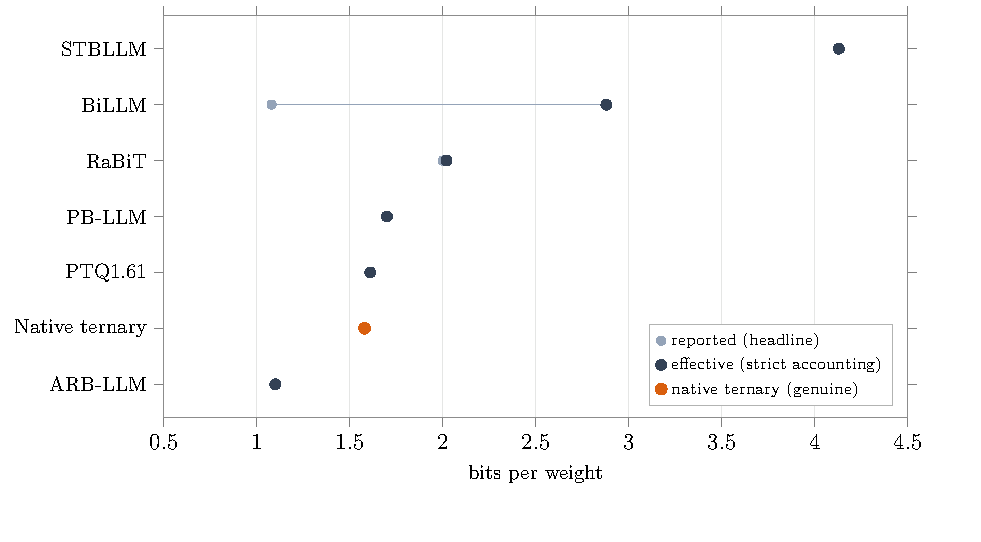
\includegraphics{fig-effbits.pdf}
\caption{Reported versus effective bits per weight. Where a strict accounting exists, the headline figure (grey) understates real storage against the effective one (dark): BiLLM's 1.08 becomes 2.88, RaBiT's nominal two bits becomes 2.02. ARB-LLM, PTQ1.61, PB-LLM, and STBLLM report only one figure. Native ternary (orange) has no such accounting gap between a deflated headline and its real storage cost: 1.58 is both nominal and effective. That is a separate question from the packed format a given kernel actually uses on disk, which for I2\_S is two bits per weight for hardware convenience, not an overhead the accounting here is missing.}
\label{fig:effbits}
\end{figure}



%% ===== 08-applications
\section{Applications and Extensions}

The native 1-bit machinery was built for text-decoder LLMs, but the period from 2024 to
2026 saw it carried into a widening set of modalities and deployment settings. This
section surveys those branches. Each is small today, but each is growing, and together
they are the fastest-moving part of the field.

\subsection{On-device and edge deployment}

The unifying theme of the area is running capable models without a data center. Concrete
demonstrations include BitNet b1.58 2B4T with open CPU and GPU inference
\cite{Ma2025-BitNet2B4T}, a 100B model at reading speed on one CPU \cite{Wang2024-1bitAIInfra}, an
inference characterization on a Raspberry Pi with BitNet Q1.58 against k-quantized
baselines \cite{Ardakani2025-LLMPi}, and analyses of when commodity CPUs beat GPUs for
on-device serving \cite{Anon2025-CPUvsGPU}. The security of the deployed weights is a
separate concern: TZ-LLM protects on-device model parameters inside an Arm TrustZone
enclave, using pipelined restoration to hide decryption latency \cite{Wang2025-TZLLM}.

\subsection{Embedding models}

Embedding models are attractive ternary targets, because the downstream operation of
approximate nearest-neighbor search tolerates quantized vectors well. A ternary-weight
fine-tuning framework with self-taught distillation preserves retrieval quality while
reducing memory and latency, and composes with approximate-nearest-neighbor indices
\cite{Chen2024-TernaryEmbedding}; Ultra-Quantisation applies 1.58-bit encodings directly to
the embedding-search problem \cite{Connor2025-UltraQuantisation}; and BitNet Text Embeddings
is a native 1-bit embedding-model family, at 0.27B and 0.6B parameters, released with
the \texttt{I2\_S} kernel path of bitnet.cpp \cite{Li2026-BitNetTextEmbeddings,web-microsoftBitNet}.

\subsection{Speech}

BitTTS quantizes both the acoustic model and the vocoder of a text-to-speech system to
1.58-bit with quantization-aware training, together with a weight-indexing scheme that
stores five ternary weights per INT8; the result is an 83\% size reduction while
improving quality over an unquantized model of the same size \cite{Kawamura2025-BitTTS}. On
the recognition side, an extremely low-bit Conformer is trained toward one bit with
co-training and stochastic precision \cite{Anon2025-OneBitASR}.

\subsection{Vision-language and vision-language-action models}

LLaVaOLMoBitnet1B was the first ternary multimodal LLM, pairing a full-precision vision
encoder with a ternary OLMo-Bitnet backbone \cite{Sundaram2024-LLaVaOLMoBitnet}. BitVLA
extends this to robotics: it builds on BitNet b1.58 2B4T, then compresses the vision
encoder to 1.58-bit weights with eight-bit activations through a quantize-then-distill
stage before robotic fine-tuning, retaining task competence at a fraction of the memory
\cite{Wang2025-BitVLA}. TernaryCLIP compresses a CLIP vision-language model to ternary weights
with distilled knowledge \cite{Zhang2025-TernaryCLIP}; TeTRA ternarizes a vision-transformer
backbone and binarizes its embedding head for compact visual place recognition on drones
\cite{Grainge2025-TeTRAVPR}; and BitMar explores low-bit multimodal fusion with an episodic
memory for edge devices \cite{Aman2025-BitMar}.

\subsection{Mixture-of-experts}

MoTE trains many ternary routed experts rather than few full-precision ones, keeping the
active-parameter budget fixed while removing the memory overhead of a full-precision
expert pool; it is competitive with a full-precision MoE-LLaVA at equal expert memory,
and the gap widens as the memory budget tightens \cite{Wang2025-MoTE}.

\subsection{Ecosystem beyond a single laboratory}

The paradigm is no longer confined to one laboratory. The Falcon-Edge family from TII,
comprising Falcon3-1.58bit models at 1B and 3B in base and instruction-tuned variants,
is trained with ternary weights during pre-training and ships a fine-tuning library
\cite{web-falconEdge}; the Spectra suites from NolanoOrg release more than 500 intermediate
TriLM checkpoints from 99M to 3.9B parameters \cite{Kaushal2024-Spectra},
\cite{Vaidhya2025-Spectra11}; and independent groups have produced binary and ternary
variants across the OPT, Llama, Qwen, and Mistral families \cite{Li2024-ARBLLM},
\cite{Dong2024-STBLLM,Xiao2025-PTQTP}.

\subsection{Environmental framing}

Several works motivate 1-bit LLMs explicitly on energy and carbon grounds
\cite{Wang2023-BitNet,Ansar2024-BEExformer}, and the reported 70\% to 96\% energy
reductions for CPU inference \cite{Wang2024-1bitAIInfra,web-bitnet2b4tCard} are the
strongest lever for that argument. A rigorous life-cycle account, one that includes the
higher training-time cost of native 1-bit models, has not yet been published and is
noted here as a gap.


%% ===== 09-reproduction
\section{Independent Re-Evaluation}\label{sec:repro}

\subsection{Rationale and scope}

The efficiency figures that motivate this paradigm are almost all author-reported and no
third party has re-checked them, including the efficiency table for BitNet b1.58 2B4T of
0.4 GB, 29 ms, and 0.028 J \cite{web-bitnet2b4tCard} and the 2.37-to-6.17-times bitnet.cpp
speedups \cite{Wang2024-1bitAIInfra}, all quoted against a half-precision baseline. This
section re-measures a small, well-defined subset of those claims on commodity hardware,
adding the 8-bit and 4-bit baselines a practitioner would actually compare against. It
verifies published claims; it does not train models or ablate methods.

\subsection{Setup}

For Arm A (the accuracy arm), we use EleutherAI's lm-evaluation-harness at commit
\texttt{b954108} (pinned 4 September 2026), on a laptop RTX 4080 with 12 GB of memory shared
with other workloads, with the batch size capped so that memory use stays within budget.
The primary pairing is BitNet b1.58 2B4T \cite{Ma2025-BitNet2B4T}, about 2.4 billion
parameters in total and 2.0 billion outside the token embedding, against
Qwen2.5-1.5B-Instruct, about 1.5 billion parameters, the full-precision model the BitNet
2B4T card itself compares against. That pairing is \textbf{not a controlled baseline}: the two
differ in parameter count, architecture, tokenizer, and training data. To address that we
add three comparisons from open checkpoints, in decreasing order of how tightly matched
they are. The cleanest is Spectra's TriLM and FloatLM at 2.4 billion parameters,
identical tokenizer, data, and 300-billion-token budget, ternary trained from scratch
against FP16 trained from scratch \cite{Kaushal2024-Spectra}. Next, Qwen2.5-1.5B-Instruct in
bf16 against a 4-bit (nf4) quantization of the same weights, which isolates the cost of
post-hoc 4-bit compression. Least tightly matched is Falcon3-1B in its 1.58-bit and its
bf16 form: TII trains the 1.58-bit model with ternary weights from pre-training and
releases a bf16 checkpoint alongside it \cite{web-falconEdge}, but does not document whether
that bf16 checkpoint is a dequantized copy of the same run or the earlier full-precision
Falcon3-1B, so this pair is matched in model family and parameter count but not
demonstrably in training data or schedule. All checkpoints are the
instruction-tuned variants where one exists, evaluated without a chat template as the
harness default; the tables abbreviate Qwen2.5-1.5B-Instruct to Qwen2.5-1.5B. The tasks
are the seven-task zero-shot suite (ARC-Easy, ARC-Challenge, HellaSwag, WinoGrande, PIQA,
OpenBookQA, and BoolQ) reported as plain accuracy, plus WikiText-2 word perplexity and
MMLU at zero shot. Each model is run once, with a HellaSwag determinism check.

MMLU is run at zero shot rather than the card's five: BitNet's native Hugging Face layer
compiles per input shape, and the fifty-seven MMLU subjects each carry a different
five-shot context length, which thrashes the compilation cache; zero shot keeps a fixed
shape and runs at the speed of the rest of the suite. GSM8K, dropped from an earlier
version of this study, is re-measured here (Section 10.3), but on its own terms: it needs
multi-step generation and the model's chat template, so it is run at five shot with the
template applied and generation to 256 tokens, and its numbers are not comparable to the
loglikelihood, template-free suite above. A build note: on Windows, that native layer only compiles at
all with a Triton build matching the installed PyTorch; without it it runs eagerly and
even the zero-shot suite is several times slower.

For Arm B (the efficiency arm), we build the reference bitnet.cpp runtime from source and run
every model through that one binary: its \texttt{I2\_S} ternary kernel serves the BitNet
checkpoint, and the llama.cpp code path it is built on serves the Qwen2.5-1.5B
baselines at five quantization levels: FP16, \texttt{Q8\_0}, and three 4-bit formats, \texttt{Q4\_0},
\texttt{Q4\_K\_S}, and the \texttt{Q4\_K\_M} k-quant that is the common default for local inference. The FP16
baseline here is an FP16 GGUF of the same Qwen checkpoint whose BF16 weights the accuracy
arm loads; the C++ runtime has no BF16 path, and the two formats are numerically close,
so the accuracy and efficiency baselines are the same model in the nearest format each
runtime supports and are not compared against each other. The 4-bit comparison is on this
one x86 machine only; a GPU, a second CPU, and quantizers outside the GGUF family such as
AWQ or GPTQ would each be needed to generalize it further. Every measurement shares a
runtime, a machine, and a harness. The machine is an Intel Core i9-14900HX laptop, eight performance cores
and sixteen efficiency cores, on AC power. We sweep threads over 1, 2, 4, 8, and 16,
take prefill at 128, 512, and 2048 tokens and decode at 128 tokens, and repeat every
point five times through the bundled \texttt{llama-bench}. Peak resident memory is sampled from the process working set
during a decode run. Energy is measured in a separate pass on battery, where the
smart-battery controller exposes whole-system power to the operating system as a
discharge rate (it reads zero on AC, and this machine has no running-average
power-limit counter); we sample that rate during a thirty-second idle window and during
a sustained decode, and divide mean power by the decode rate. The energy pass covers the
ternary model and the half-precision, 8-bit, and 4-bit k-quant baselines. On battery the
processor runs at a lower power limit, and that limit tightens as the battery drains, so
the pass is slower than the plugged-in sweep, absolute energy figures drift across runs,
and only within-run model-to-model ratios are compared.

Three notes on getting the runtime to work. It does not link as a shared library on this
toolchain, because the core ggml library references an \texttt{I2\_S} quantizer symbol that lives
only in the CPU backend; a static build resolves it. Its BitNet feed-forward activation
is set to SiLU where BitNet b1.58 2B4T uses a gated squared-ReLU, which we changed and
rebuilt (Section 10.3); the throughput figures are the same either way. And the \texttt{TL2}
lookup-table kernel, which needs a per-shape code-generation step shipped only for older
BitNet sizes, was not exercised, so the ternary figures are \texttt{I2\_S} only. We built
microsoft/BitNet at commit \texttt{0b341e5}, whose \texttt{3rdparty/llama.cpp} submodule was at
commit \texttt{390c307}; the one-line fix changes \texttt{LLM\_FFN\_SILU} to \texttt{LLM\_FFN\_RELU\_SQR} in
\texttt{src/models/bitnet.cpp}.

\subsection{Accuracy results}

Table \ref{tab:acc-primary} reports, for the primary pairing, plain accuracy on the
seven-task zero-shot suite, its mean, WikiText-2 word perplexity at a 2048-token stride,
and MMLU at zero shot. Both HellaSwag determinism checks reproduced to the last digit across two
independent runs. Accuracy is the unnormalized figure (\texttt{acc}); we report it rather than
the length-normalized \texttt{acc\_norm} so that one metric is used across all seven tasks. For
HellaSwag the two diverge widely, \texttt{acc\_norm} is 67.6 for BitNet and 68.3 for Qwen,
because the endings vary in length and an unnormalized log-likelihood favors the shorter
ones; this is why the HellaSwag column reads near 50 while the vendor's length-normalized
figure is near 68, and why the C++ runtime's own HellaSwag scorer (Table \ref{tab:quant-cost}),
which averages log-probability per ending token, lands between the two at about
62 to 66. The metric, not the runtime, accounts for the gap.

\begin{table}[htbp]\centering
\caption{Independent accuracy re-measurement of the primary pairing: unnormalized accuracy (\emph{acc}) on the seven-task zero-shot suite with its mean, WikiText-2 word perplexity at a 2048-token stride, and MMLU at zero shot. One run per model, with a HellaSwag determinism check. HellaSwag's unnormalized \emph{acc} reads near 50 for both models by design (an unnormalized log-likelihood favors shorter endings, discussed below); the length-normalized \emph{acc\_norm} both vendors and papers usually quote is near 68 for both.}
\label{tab:acc-primary}
\footnotesize
\begin{tabularx}{\linewidth}{Lllllllllll}\toprule
model & ARCe & ARCc & HS & WG & PIQA & OBQA & BoolQ & mean & ppl & MMLU \\
\midrule
BitNet b1.58 2B4T (W1.58, 2.4B) & 76.8 & 47.0 & 50.7 & 72.5 & 77.0 & 30.8 & 79.0 & 61.98 & 16.67 & 52.07 \\
Qwen2.5-1.5B-Instruct (BF16, 1.5B) & 76.7 & 43.6 & 50.9 & 62.7 & 76.3 & 31.8 & 78.0 & 60.00 & 13.48 & 60.03 \\
\bottomrule\end{tabularx}\end{table}

Two comparisons matter. First, against the vendor figure: the BitNet b1.58 2B4T model
card reports a headline ``zero-shot average'' of 54.19, below our 61.98 on the seven-task
suite and below its own reference Qwen. That figure averages a broader set that includes
MMLU and GSM8K, and most of the difference is MMLU. Our zero-shot MMLU, 52.07 for BitNet
against 60.03 for Qwen, closely tracks the card's five-shot values (53.17 and 60.25) under a
different protocol, and matches its
roughly eight-point deficit: the ternary model is competitive on commonsense reasoning
but clearly behind on world knowledge, and any average that folds MMLU in inherits that
gap. A single vendor ``average'' is not portable across evaluation setups; per-task numbers
are the only safe unit of comparison.

Second, the controlled comparisons. The BitNet-versus-Qwen pairing is not size- or
training-matched, so we ran three pairs from open artifacts that are, each in its own
right (Section 10.2):

\begin{table}[htbp]\centering
\caption{Three pairs from open checkpoints, in decreasing order of how tightly matched they are: change in seven-task mean, WikiText-2 perplexity, and zero-shot MMLU for the ternary or 4-bit member against its full-precision counterpart.}
\label{tab:acc-controlled}
\footnotesize
\begin{tabularx}{\linewidth}{LLLlLl}\toprule
pair (most to least matched) & ternary or 4-bit & full precision & $\Delta$ mean & ppl & $\Delta$ MMLU \\
\midrule
Spectra 2.4B, native ternary vs FP16 (300B tok) & TriLM 51.49 & FloatLM 52.05 & -0.56 & 14.90 vs 13.06 & -2.2 \\
Qwen2.5-1.5B, nf4 4-bit vs bf16 & 57.33 & 60.00 & -2.67 & 14.59 vs 13.48 & -2.0 \\
Falcon3-1B, 1.58-bit vs bf16 (checkpoint relation undocumented) & 45.69 & 57.22 & -11.53 & 32.82 vs 18.85 & -18.4 \\
\bottomrule\end{tabularx}\end{table}

Three things follow (Fig. \ref{fig:controlledpairs} plots the three pairs' seven-task means
against each other directly). The Spectra pair, the cleanest test, puts native ternary within
0.6 points of FP16 on the seven-task mean at 2.4 billion parameters, with perplexity 14\%
higher: downstream parity alongside a worse language-modeling loss, the exact shape the
native-training literature reports for itself (Section 8.2), now measured under a matched
protocol rather than inferred. Both Spectra models score near chance on MMLU, so that
column is uninformative for this pair; the 300-billion-token budget simply does not buy
world knowledge at 2.4 billion parameters. Second, post-hoc 4-bit quantization of Qwen
costs 2.7 points on the mean and 2.0 on MMLU, more than native ternary loses at a
comparable scale, consistent with the ParetoQ finding that ternary quantization-aware
training sits ahead of four-bit post-training quantization on the size-accuracy frontier
(Section 8.3).

Third, and this is the part that most constrains how far the parity result generalizes,
the Falcon3-1B pair loses heavily: 11.5 points on the seven-task mean, a 74\% higher
perplexity, and MMLU driven to chance. This pair cannot separate a scale effect from a
training-recipe one, both because it is at one-billion rather than multi-billion
parameters and because its two checkpoints are not demonstrably matched in training data
(Section 10.2). What it does establish is a clean negative: the 1.58-bit format at the
one-billion-parameter scale does not inherit the parity that native ternary shows at 2.4
billion, though with the checkpoint match unresolved, that negative could reflect the
pair's mismatch as readily as it could reflect scale. Taken together, the two pairs that
are matched closely enough to compare are consistent with parity being a property of
native ternary pre-training carried out at multi-billion scale rather than a general
consequence of constraining weights to 1.58 bits, but two pairs, one of them confounded,
do not establish that on their own; whether it holds above the roughly 2B, 4T-token
ceiling at which it has been measured is the open question of Section 11.1. The uncontrolled
BitNet-versus-Qwen result, a slight lead for the 2B ternary model on the seven-task mean
and a deficit on perplexity and MMLU, sits consistently between the Spectra and the 4-bit
pairs.

GSM8K is the one benchmark the seven-task suite leaves out, because it needs multi-step
generation rather than a single loglikelihood; we re-measure it separately, at five shot
with each model's chat template and greedy generation to 256 tokens (Table \ref{tab:gsm8k}).
The two extraction rules that the standard harness reports are worth keeping apart:
flexible-extract takes the last number in the output, strict-match accepts only the
canonical answer line. For BitNet and the full-precision Falcon3-1B the two nearly agree;
for the other models they diverge sharply, the model reaching a right answer but not
ending in the canonical form, so the flexible figure is the one that tracks arithmetic
ability and the one we compare on. On it, three things follow. First, the vendor's
GSM8K claim reproduces in direction: BitNet b1.58 2B4T scores 61.9 against our own Qwen2.5-1.5B's 57.5,
a 4.4-point lead where the card reports a 1.6-point one (58.38 against 56.79), so the one
benchmark on which the card puts the 1-bit model ahead holds up under an independent run.
Second, the 4-bit nf4 quantization of Qwen costs 7.8 points on GSM8K, against 2.7 on the
seven-task mean: arithmetic is more fragile under post-hoc quantization than commonsense
reasoning is. Third, the controlled 1B and 2.4B pairs behave as they did elsewhere, the
1.58-bit Falcon3-1B losing 17 points against its bf16 form and both Spectra models sitting
at the GSM8K noise floor, uninformative for that pair exactly as MMLU was.

\begin{table}[htbp]\centering
\caption{GSM8K exact-match accuracy at five shot, with generation and the chat template for the instruction-tuned models above the rule (the Spectra base models below the rule carry no template, are run template-free, and sit at the GSM8K noise floor rather than being meaningfully tested). flexible-extract takes the last number in the output; strict-match accepts only the canonical answer line. These numbers use a different protocol from the loglikelihood suite of Table \ref{tab:acc-primary} and are not folded into any mean.}
\label{tab:gsm8k}
\footnotesize
\begin{tabularx}{\linewidth}{LLL}\toprule
model & flexible-extract & strict-match \\
\midrule
BitNet b1.58 2B4T & 61.9 & 59.6 \\
Qwen2.5-1.5B-Instruct, bf16 & 57.5 & 35.0 \\
Qwen2.5-1.5B-Instruct, nf4 4-bit & 49.7 & 36.8 \\
Falcon3-1B-Instruct, bf16 & 44.7 & 42.6 \\
Falcon3-1B-Instruct, 1.58-bit & 27.7 & 7.4 \\
\midrule
Spectra TriLM 2.4B, no template & 3.0 & 1.9 \\
Spectra FloatLM 2.4B, no template & 1.9 & 1.3 \\
\bottomrule\end{tabularx}\end{table}

We separately checked the accuracy cost of the quantizations used in the efficiency arm,
running WikiText-2 perplexity and a HellaSwag subset (the first 1000 of 10042 items)
through the C++ runtime's own batched evaluators (\texttt{llama-perplexity}, whose HellaSwag
mode averages log-probability per ending token) so the three Qwen levels are measured
against each other under one scorer. This is a narrow check, two metrics rather than the
full seven-task suite, and it is not a substitute for running that suite on the 4-bit
model, which the runtime's harness does not support. Quantizing the baseline is cheap on
these two tasks: the 8-bit build costs 0.1\% on perplexity, and the 4-bit k-quant costs
4.5\% on perplexity (9.25 against 8.85). On the HellaSwag subset the observed differences
were small, 0.5 points for the 8-bit build and 0.3 for the 4-bit k-quant against half
precision's 65.3\%, within the
marginal confidence intervals; we did not run a paired significance test, so this rules
out a large accuracy drop but not a small one.

\begin{table}[htbp]\centering
\caption{Accuracy cost of the GGUF quantizations used in the efficiency arm, scored through the C++ runtime's own batched evaluators so the three Qwen levels are measured alike: WikiText-2 perplexity and a 1000-item HellaSwag subset.}
\label{tab:quant-cost}
\footnotesize
\begin{tabular}{lll}\toprule
model & WikiText-2 ppl & HellaSwag (n=1000) \\
\midrule
Qwen2.5-1.5B, FP16 & 8.85 & 65.3\% \\
Qwen2.5-1.5B, \texttt{Q8\_0} & 8.86 & 65.8\% \\
Qwen2.5-1.5B, \texttt{Q4\_K\_M} & 9.25 & 65.6\% \\
\bottomrule\end{tabular}\end{table}

The BitNet checkpoint needed a source fix to the runtime before it produced sensible
output at all. Built from the project as documented (commit \texttt{0b341e5}, \texttt{llama.cpp}
submodule at \texttt{390c307}, Section 10.2), the runtime's BitNet graph selects a SiLU
feed-forward activation, whereas BitNet b1.58 2B4T uses a gated squared-ReLU (its
released configuration sets the feed-forward activation to squared-ReLU); this is an open
issue in the project. The fix is a one-line change to the activation selector in the
BitNet model source, from SiLU to squared-ReLU (\texttt{LLM\_FFN\_SILU} to \texttt{LLM\_FFN\_RELU\_SQR} in
\texttt{src/models/bitnet.cpp}). Left uncorrected, WikiText-2 perplexity through the runtime is 86.9 and
HellaSwag is 38.7\%, far below any working model. Changing that one line and rebuilding
brings token-level WikiText-2 perplexity to 12.99 and HellaSwag
to 62.4\%, both in line with the transformers implementation of the same weights (16.67
word-level perplexity, HellaSwag near 62 to 68 depending on the metric); the throughput
and memory figures of Section 10.4 are unchanged, since a squared-ReLU costs no more than
a SiLU. The released weights are therefore sound; the defect we traced is in the reference
runtime, not the checkpoint, though it is not the only rough edge we found there (below),
and we did not catch it until the results were scrutinized. One report questions
the checkpoint itself, reading its 1,187,801,280-byte size as a truncated re-upload with
empty feed-forward tensors \cite{web-bitnetIssue608}; this is
the shared-embedding layout, in which the model keeps no separate output projection, and
a checkpoint with zeroed feed-forward weights could not reach a perplexity in the low
teens under any activation, so that reading is inconsistent with the result here. The
file used is pinned to Hugging Face revision \texttt{a1f2f1c765812aa8af3f6eda4a313707064bba15},
SHA-256 \texttt{4221b252fdd5fd25e15847adfeb5ee88886506ba50b8a34548374492884c2162}. A separate,
minor issue remains: the GGUF omits the \texttt{tokenizer.ggml.pre} field, so the runtime warns
and falls back to a default pre-tokenizer; we did not run a matched-tokenization check
to isolate its effect, but the activation-corrected perplexity and HellaSwag scores
landing in the expected range suggest it is small. The two runtime perplexities that can be
stated, 12.99 from llama.cpp and 16.67 from transformers (the accuracy table above), are
not directly comparable, since one is a token-level and the other a word-level figure on
different tokenizations; both are in the range the model card implies.

\subsection{Efficiency results}

Table \ref{tab:efficiency}, and Fig. \ref{fig:efficiency}, report decode throughput, prefill throughput,
on-disk size, and peak resident memory. The Qwen baseline is shown at four 4-bit and
low-bit settings, \texttt{Q4\_0}, \texttt{Q4\_K\_S}, \texttt{Q4\_K\_M}, and \texttt{Q8\_0}, plus FP16, so the 4-bit comparison
does not hinge on one format. Throughput is
reported at a common four-thread operating point: that is BitNet's own decode optimum on
this hybrid-core part, and holding it fixed keeps the comparison on one setting. It is
not the global optimum for every model, so we also give each model its own best point
below, and the ordering is the same either way. Prefill is the 512-token point; decode
generates 128 tokens; each throughput figure is the mean of five repeats, with the
standard deviation shown. Disk size is exact; peak resident memory is a single sample
taken at eight threads and is essentially thread-independent.

\begin{table}[htbp]\centering
\caption{Independent efficiency re-evaluation on one x86 laptop at a common four-thread operating point: decode and prefill throughput (mean of five repeats, standard deviation in parentheses), on-disk size, and peak resident memory, for the BitNet \texttt{I2\_S} checkpoint and Qwen2.5-1.5B at five GGUF quantization levels.}
\label{tab:efficiency}
\footnotesize
\begin{tabularx}{\linewidth}{LLLlL}\toprule
configuration & decode tok/s & prefill tok/s & disk (GiB) & peak RAM (GB) \\
\midrule
BitNet b1.58 2B4T, \texttt{I2\_S} & 28.6 (1.6) & 108.9 (5.2) & 1.10 & 1.22 \\
Qwen2.5-1.5B, \texttt{Q4\_0} & 36.3 (1.1) & 116.1 (0.8) & 0.99 & 1.66 \\
Qwen2.5-1.5B, \texttt{Q4\_K\_S} & 28.7 (4.8) & 109.4 (5.4) & 1.00 & 1.64 \\
Qwen2.5-1.5B, \texttt{Q4\_K\_M} & 33.8 (0.3) & 107.6 (2.7) & 1.04 & 1.60 \\
Qwen2.5-1.5B, \texttt{Q8\_0} & 24.1 (0.1) & 72.4 (3.1) & 1.76 & 1.64 \\
Qwen2.5-1.5B, FP16 & 14.4 (0.3) & 70.9 (0.8) & 3.31 & 3.02 \\
\bottomrule\end{tabularx}\end{table}

Against FP16 the vendor's direction reproduces: the ternary model decodes 1.99 times as
fast, close to the roughly 2.2-times ratio the card's own table implies. The memory
claim does not carry over as stated: the card's 0.4 GB against 2.6 GB, a 6.5-times
advantage, is a weights-only, non-embedding accounting, whereas the running process
needs 1.22 GB against FP16's 3.02 GB once the 128k-vocabulary embedding, the key-value
cache, and the compute buffers are counted, a 2.5-times advantage. Absolute decode is
35 ms per token against the card's 29 ms, consistent given a different processor.

A comparison closer to deployment is against the 4-bit builds people actually run
locally, and against every one of them, on this machine, the ternary model has no
decode-speed or disk-size advantage and only a narrow memory one. At the common
four-thread point it decodes no faster than any of the three 4-bit formats and slower
than two of them: 28.6 tokens per second against 36.3 for \texttt{Q4\_0}, 33.8 for \texttt{Q4\_K\_M}, and
28.7 for \texttt{Q4\_K\_S}, whose four-thread run was noisy and which reaches 33.8 at eight
threads. All three 4-bit builds are smaller on disk (0.99 to 1.04 GiB against 1.10) and
tie or beat it on prefill. The ternary model does keep a resident-memory edge, 1.22 GB
against 1.60 to 1.66 GB, about 24 to 27\%. Giving each model its own best thread count
does not change the ordering: BitNet's fastest decode is 28.6 at four threads, while
\texttt{Q4\_0} reaches 36.3 at four and the two k-quants reach 33.8 to 34.2 at eight; BitNet's
fastest 512-token prefill is 112 at eight threads against 116 to 132 for the 4-bit
formats at their best. Its 2.4B parameters, only 2.0B of them outside the token
embedding (Section 10.2), are why: a naive estimate from parameter count and nominal
bit-width alone, 2.4B at roughly 1.6 bits, predicts under half a gigabyte, well below
the measured 1.10 GiB. The gap is the token-embedding table, which is not
ternary-packed and is a larger share of this smaller model's parameters than Qwen's
embedding is of its own 1.5B; that overhead, not a straightforward bit-width trade-off,
is most of why the two on-disk sizes land so close together. Against \texttt{Q8\_0} the picture is intermediate: 1.19
times on decode, 0.74 times on memory. Decode throughput for every model peaks at four
or eight threads on this hybrid-core part and falls off at 16 as the efficiency cores
and memory bandwidth become the limit; prefill for every model keeps scaling to 8 or 16
threads. The 2.37-to-6.17-times bitnet.cpp speedups quoted elsewhere
\cite{Wang2024-1bitAIInfra} are measured against FP16 at 3B parameters and above; this 2B,
x86 point sits below that band, and against a 4-bit baseline on this machine it inverts
for all three formats tested. Whether it also inverts on a GPU or a different CPU is not
tested here.

The battery pass covers the ternary model and the 4-bit k-quant (\texttt{Q4\_K\_M}), the 8-bit
build, and half precision, run three times across two battery-discharge sessions. On
battery the processor runs at a lower power limit and that limit tightens as the battery
drains, so whole-system energy per token drifts across runs, the ternary model measuring
1.9, 2.4, and 2.8 J per token in the three, and only the model-to-model ratios within a
run are stable. Those ratios are consistent. In the mid-range run the ternary model and
the k-quant both cost about 2.4 J per token, the 8-bit build about 3.8, and half
precision about 5.3; across all three runs the ternary model sat at 0.88 to 1.00 times
the energy of the k-quant, 0.59 to 0.69 times the 8-bit build, and 0.40 to 0.46 times
half precision. The energy ranking follows the decode-throughput ranking exactly: the
ternary model and the k-quant emit tokens fastest, so they amortize the machine's large
idle draw, 29 to 49 W depending on battery state, over the most tokens. Against the 4-bit
k-quant, then, the ternary model has no energy-per-token advantage on this machine, the
same result the decode-speed and disk-size comparisons give; its advantage is a little
over half off against half precision and roughly a third off against the 8-bit build, and
that is a speed effect, not a lower compute cost. An idle-subtracted compute-energy
figure did not reproduce across runs, since the idle draw itself varied by almost 20 W
between sessions and on a draining battery some model runs drew less than the bracketing
idle windows, so only whole-system energy is reported. None of these whole-laptop figures
is comparable to the model card's 0.028 J, which is a CPU-side, non-embedding number.

\subsection{Summary of findings}

On the accuracy arm, five things held. Every released checkpoint loaded and ran under a
single pinned harness with no code changes beyond a Windows Triton pin. Every determinism
check reproduced exactly. The controlled Spectra pair put native ternary within 0.6
points of FP16 on the seven-task mean at 2.4 billion parameters, with a 14\% higher
perplexity, so the ``downstream parity, worse language-modeling loss'' pattern of the
native-training literature reproduces under a matched protocol, not just in the
uncontrolled vendor pairing. Our zero-shot MMLU, 52.07 for BitNet b1.58 2B4T against
60.03 for Qwen, closely tracks the card's five-shot values under a different protocol
and matches its roughly eight-point
world-knowledge deficit. And GSM8K, re-measured with generation and the chat template,
reproduces in direction the one benchmark on which the card leads: BitNet b1.58 2B4T scores 61.9 to
our Qwen's 57.5 on flexible-extract (Section 10.3).

What the controlled comparisons also show is a cost, and a boundary on the claim. Post-hoc
4-bit quantization of Qwen loses 2.7 points on the seven-task mean and 7.8 on GSM8K, more
than native ternary loses at a similar scale. The 1.58-bit Falcon3-1B pair loses far more,
11.5 points on the mean, 17 on GSM8K, and essentially all of MMLU; that pair does not
isolate scale from training recipe (Section 10.3), but it does show that constraining
weights to 1.58 bits at the one-billion-parameter scale does not by itself deliver parity.
Parity, where we see it, is a property of native ternary pre-training at multi-billion
scale, and even there it is downstream parity with a worse language-modeling loss, not
equivalence. Whether it survives above the measured regime is still untested (Section 11.1).

One vendor number is not directly comparable rather than reproduced or refuted: the
BitNet b1.58 2B4T model card's single headline ``zero-shot average'' of 54.19. Our
seven-task suite gives 61.98, but the card's figure is an average over a different and
broader task set, taken with the chat template we did not apply, so the two cannot be
placed side by side. It is a concrete instance of a vendor summary statistic that a
reader cannot check without reconstructing the exact task list and prompt format.

On the efficiency arm the headline result is that, on this commodity x86 machine, a
standard 4-bit quantization of the full-precision baseline matches or beats the flagship
1-bit model on every axis a practitioner would weigh except one. Against all three 4-bit
builds the ternary model shows no decode-speed advantage (it is slower than two of them
and ties the third) and no on-disk-size advantage; against the 4-bit k-quant it shows no
energy-per-token advantage either, the two within 0 to 12\% across three battery runs
(Section 10.4). Its one retained edge is a 24-to-27\% smaller resident set. On the two
accuracy tasks that could be scored through the same runtime the k-quant stays close
(Section 10.3). All of this holds whether threads are fixed at four or tuned per model.

The vendor's own comparisons, made only against FP16, do reproduce in direction: the
roughly 2-times decode advantage over FP16 holds, the 6.5-times memory advantage becomes
2.5-times once memory is counted as resident set rather than non-embedding weights, and
whole-system energy per token is about 0.43 times FP16, tracking the decode-speed ratio.
Against \texttt{Q8\_0} the decode edge is 1.2-times and the energy ratio about 0.6-times, again a
speed effect. So the paradigm's efficiency case at this scale holds against half
precision and against \texttt{Q8\_0}, but not against any of the tested 4-bit builds; it is also a
case about these released checkpoints and this one machine, not a general property of
the representation, since the comparison pairs a 2.4B ternary model against a 1.5B
full-precision one and cannot separate the two. We did not test a GPU or a second
machine; Section 10.7 discusses how far this is likely to carry.

Two further findings came out of the efficiency arm. The 4-bit k-quant of the baseline
costs 4.5\% on perplexity and, on the 1000-item HellaSwag subset, a difference of 0.3
points that we did not test for significance (Section 10.3), so the faster, smaller
k-quant stays close in accuracy on the tasks checked. And the reference CPU runtime,
built from the project as documented, does not produce correct output for BitNet b1.58
2B4T until a source constant is changed: its BitNet graph applies a SiLU feed-forward
activation where the model uses gated squared-ReLU, a known open issue. Uncorrected,
WikiText-2 perplexity is 86.9 and HellaSwag 38.7\%; the one-line fix brings these to
12.99 and 62.4\% (Section 10.3). The released weights are sound. The throughput and
memory figures of Section 10.4 are unchanged by the fix, since a squared-ReLU is no more
costly than a SiLU and the activation is a negligible fraction of the per-token work.

Two benchmarks that an earlier version of this study left out are now re-measured. MMLU,
dropped because five-shot evaluation thrashed BitNet's per-shape compilation cache, is
re-measured at zero shot; GSM8K, which needs generation and a chat template rather than
the loglikelihood path used for everything else, is re-measured at five shot with the
template and reported separately (Section 10.3). Both reproduce the corresponding vendor
figures. Nothing in the accuracy arm now rests on an unverified vendor number.

\subsection{Reproducibility audit}

For the checkpoints in the accuracy arm we record, as a by-product, what license
governs reuse, whether the weights load under a stock harness, and whether our numbers
land near the vendor's. The controlled-comparison checkpoints of Section 10.3, the
Spectra TriLM and FloatLM pair, Falcon3-1B in bf16, and the nf4 quantization of Qwen,
all loaded through the stock \texttt{AutoModelForCausalLM} path with no special handling and are
not repeated in Table \ref{tab:repro-audit}.

\begin{table}[htbp]\centering
\caption{Reproducibility audit for the accuracy-arm checkpoints: governing license, whether the weights load under a stock harness, and whether our measurements land near the vendor's.}
\label{tab:repro-audit}
\footnotesize
\begin{tabularx}{\linewidth}{LLLL}\toprule
checkpoint / artifact & license & loads and runs & reproduces \\
\midrule
BitNet b1.58 2B4T, bf16 weights (transformers) & MIT & yes & per-task yes, headline average no \\
BitNet b1.58 2B4T, released \texttt{I2\_S} GGUF (bitnet.cpp) & MIT & only after a source patch & yes once patched (ppl 12.99) \\
Falcon3-1B-Instruct-1.58bit & Falcon LLM License 2.0 & yes & no public per-task baseline \\
Qwen2.5-1.5B-Instruct & Apache-2.0 & yes & full-precision reference \\
\bottomrule\end{tabularx}\end{table}

The BitNet rows are the point of this audit. The bf16 weights load as a native
transformers model type, so the model card's \texttt{trust\_remote\_code} instruction is stale,
and on Windows the layer compiles only against a matched Triton build; run that way the
model is competitive (Section 10.3). The released
GGUF, which is the only artifact that delivers the efficiency the whole approach is for,
loads but returns near-broken output from the reference runtime as built, because that
runtime applies the wrong feed-forward activation to this model (Section 10.3); a
one-line source change fixes it, but a practitioner following the documented build would
not know to make it. The released weights themselves are sound. Falcon3 and Qwen load
through the stock \texttt{AutoModelForCausalLM} path with no special handling. License terms
vary across the corpus, with MIT, Apache, and vendor-specific licenses all appearing,
which matters for any downstream reuse. A full audit across every released model in the
corpus is beyond this paper's scope.

\subsection{Threats}

Both arms run on a single laptop. For accuracy the GPU is shared with other workloads,
which we mitigate with a fixed batch size and off-peak scheduling; for efficiency the
machine runs under its default thermal and power policy, so the absolute throughput
figures are specific to that part and not a controlled-environment measurement. The
energy figures are coarser still: the discharge-rate sensor is noisy, the on-battery
power limit falls as the battery drains so absolute per-token energy drifts across runs,
and the numbers are whole-system rather than package or component; they support the
within-run model-to-model ratios (Section 10.4) but not an absolute claim, and we do not
report an idle-subtracted figure because it did not reproduce. The author-reported baselines cannot be matched exactly, and benchmark
contamination is a risk in heavily fine-tuned small models, which we note per model.

The efficiency findings are for a CPU datapath and may not transfer to a GPU, and the
transfer is worth reasoning about because the strong claim, that a 4-bit build is at
least as good, could plausibly flip. On a GPU neither ternary nor 4-bit weights map to a
native matrix-multiply instruction: both are unpacked to a supported floating-point or
integer type and run on the tensor cores, or go through a custom kernel. The decode-time
benefit that low-bit weights capture on CPU is memory-bandwidth, and that benefit exists
on GPU too and accrues to a 4-bit kernel as much as to a ternary one, so the CPU result
that a 4-bit kernel captures it is a reasonable prior for the GPU case. Two things could
still separate them there. A ternary-specific GPU kernel that exploits the zero state or
a sub-1.6-bit packing (Section 7.3) might pull ahead of the tuned 4-bit kernels now
standard for served inference, in a way the general-purpose CPU path does not expose.
And prefill and high-batch decode are compute-bound rather than bandwidth-bound, so their
ordering need not follow the single-stream decode ordering measured here. We tested none
of this, and a GPU comparison against a production 4-bit kernel is the obvious next step.

Every part of this reproduction is pinned to a specific commit or file rather than a
moving target: the evaluation harness at commit \texttt{b954108} (Section 10.2); microsoft/BitNet
at commit \texttt{0b341e5} with its \texttt{llama.cpp} submodule at \texttt{390c307} and the one-line
\texttt{LLM\_FFN\_SILU}-to-\texttt{LLM\_FFN\_RELU\_SQR} activation fix (Section 10.3); and the BitNet GGUF
checkpoint by Hugging Face revision and SHA-256 (Section 10.3). The Qwen GGUF builds were
produced with \texttt{llama-quantize} from one pinned FP16 GGUF, and the nf4 quantization with
bitsandbytes 0.50.2. Every accuracy and efficiency number reported in this section is the
direct output of that pinned pipeline on the machine described in Section 10.2, run once
per configuration except where a repeat count is stated. The pipeline itself, every run
script, the raw per-configuration logs behind every number in this section, and the
pinned environment files above, is at
\href{https://github.com/habibullahmanzoor/1-Bit-Survey}{https://github.com/habibullahmanzoor/1-Bit-Survey}.



\begin{figure}[htbp]
\centering
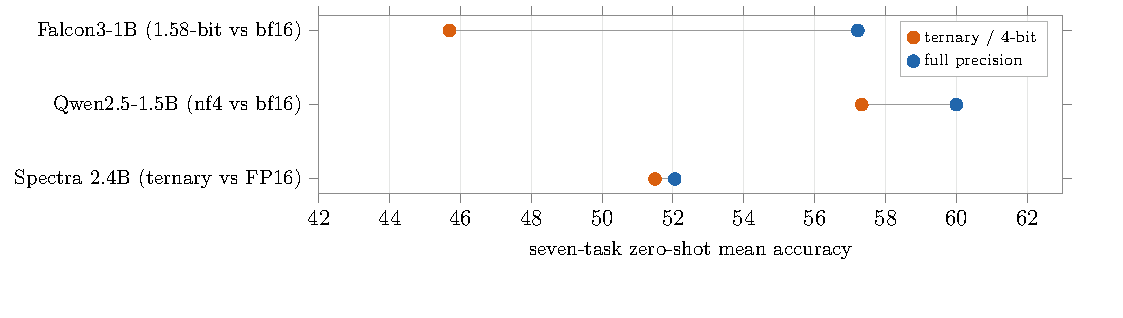
\includegraphics{fig-controlledpairs.pdf}
\caption{The three controlled pairs of Table~\ref{tab:acc-controlled}: seven-task zero-shot mean for each ternary or 4-bit model (orange) against its full-precision counterpart (blue), in decreasing order of match quality. The Spectra pair lands within 0.6 points; the least-matched Falcon3-1B pair loses 11.5.}
\label{fig:controlledpairs}
\end{figure}


\begin{figure}[htbp]
\centering
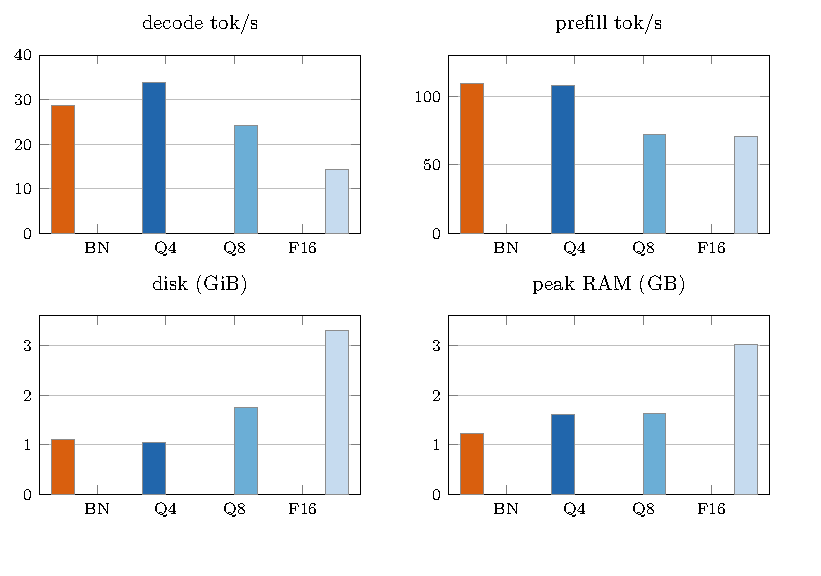
\includegraphics{fig-efficiency-bars.pdf}

\vspace{3mm}
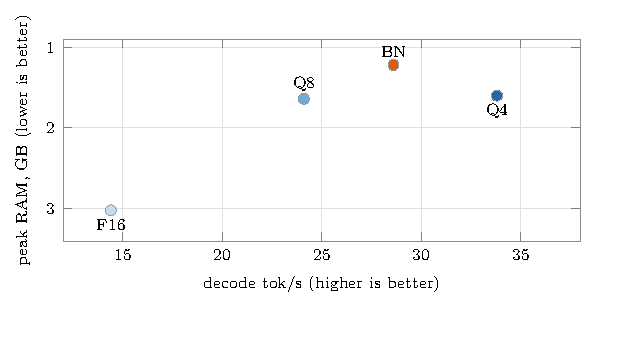
\includegraphics{fig-efficiency-scatter.pdf}
\caption{Independent efficiency re-evaluation on one x86 laptop: decode throughput (mean of five repeats at a common four-thread point), on-disk size (exact), and peak resident memory (a single sample at eight threads, essentially thread-independent). BN (orange) is the BitNet b1.58 2B4T \texttt{I2\_S} checkpoint; Q4, Q8, and F16 (blues) are Qwen2.5-1.5B-Instruct at \texttt{Q4\_K\_M}, \texttt{Q8\_0}, and FP16. The bottom panel plots decode throughput against peak memory: BitNet and Q4 share the Pareto frontier, while Q8 and F16 are dominated on both axes.}
\label{fig:efficiency}
\end{figure}



%% ===== 10-open-problems
\section{Challenges and Open Problems}

Each of the following is stated as a gap that could be closed, not as a wish list.

\subsection{The capacity ceiling and its dependence on the token budget}

The first open problem is whether the full-precision parity of BitNet b1.58 is a
property that survives to frontier scale and token budgets, or an artifact of the two-
to four-trillion-token regime in which it has been measured. The two bodies of evidence
point in opposite directions, though, as Section 6.6 notes, they measure different
quantities: precision-aware scaling laws and the quantization-induced degradation study
are about post-training quantization of a fixed model, and find that its degradation
grows with training tokens, projecting that a model quantized to low bits after being
trained on 20 to 100 trillion tokens would fall progressively further behind its FP16
source \cite{Kumar2024-ScalingLawsPrecision,Ouyang2024-QiDScaling}. These findings motivate
testing whether an analogous degradation appears in native ternary training itself, at
frontier token counts; they do not, by themselves, establish that it will. The native
ternary suites and ParetoQ report the opposite trend
within their range: ternary improves on a bits-for-bits basis as data scales, and a
600M ParetoQ ternary model beats a 3B prior-state-of-the-art ternary model
\cite{Kaushal2024-Spectra,Vaidhya2025-Spectra11,Liu2025-ParetoQ}. Our controlled re-run
of Spectra's matched pair (Section 10.3) confirms downstream parity at 2.4B parameters
and 300B tokens, with a 14\% higher perplexity, but that is well inside the measured
regime. These findings have not been reconciled, because no native 1-bit model has been
trained at both a frontier parameter count and a frontier token count. This is the single
most important experiment that the field is missing, and it is expensive but not
prohibitively so.

\subsection{Training stability at frontier scale}

The second open problem is whether native 1.58-bit pre-training becomes unstable, with
loss spikes or divergence, once the model is much larger than today's and the token
budget grows with it, and whether the current mitigations only delay that instability.
The largest reported native run is 4T tokens at 2B parameters \cite{Ma2025-BitNet2B4T}, so
every stability claim in the literature is at or below that scale; a 20B or 200B native
model on tens of trillions of tokens is untried. Continual quantization-aware training
already documents loss spikes at the full-precision-to-1.58-bit transition and partial
fixes, namely optimizer-state retention and a quantization warmup
\cite{Nielsen2025-ContinualQAT,Tu2025-Rethink1bitOpt}, and the deadzone-trapping analysis
of Tequila and the gated low-rank correction of HGF address related instabilities
\cite{Huang2025-Tequila,Anon2026-HGF}. Whether these mitigations compose into a stable run
an order of magnitude larger is unknown.

\subsection{The activation-precision floor}

The third open problem is whether four bits is the practical floor for activations
alongside roughly one-bit weights, or whether rotation together with sparsification can
reach two-bit activations. Native A4 is solved by hybrid quantization and sparsification
\cite{Wang2024-BitNetA48} and by an online Hadamard transform \cite{Wang2025-BitNetV2};
post-training quantization mostly reaches A6 \cite{Zhao2026-BWLA,Ye2025-DBellQuant}, with
one single-preprint report of A4 through rotation \cite{Zhao2026-TWLA} not yet corroborated;
and QuEST
demonstrates one-bit weights and activations but only below 1B parameters
\cite{Panferov2025-QuEST}. Nobody has demonstrated W1.58A2 at multi-billion scale with
acceptable accuracy. Given that activation traffic now dominates once weights occupy
roughly one bit, this is where the next efficiency step must come from.

\subsection{A theory of straight-through training}

The fourth open problem is the absence of a general convergence theory for
straight-through training of 1-bit Transformers; only special cases are understood. CAGE
proves convergence for its curvature-corrected estimator in the smooth non-convex
setting \cite{Tabesh2025-CAGE}; a kernel-limit analysis proves a scaling law for 1-bit
networks as width grows \cite{Daliri2024-Theory1bit}; and precision-expressivity trade-offs
are being formalized \cite{Anon2026-EveryBitCounts,Anon2026-ExpressivePowerWQ}. What is
missing is an account that connects the estimator bias to the observed instabilities and
predicts which schedules and estimators avoid them.

\subsection{Hardware co-design}

The fifth open problem is that no shipping processor exposes a ternary
matrix-multiplication primitive, and only five works in the corpus co-design across
algorithm, kernel, and hardware \cite{Ma2024-BitNetB158,Ma2025-BitNet2B4T},
\cite{Zhu2024-MatmulFree,Zhang2026-SparseBitNet,Ji2024-BMTBAT}. The accelerator
literature on lookup-table ASICs, compute-in-ROM, processing-in-memory, and edge FPGAs
\cite{Shan2025-Platinum,Guan2026-TOM,Malekar2025-PIMLLM,Qiao2025-TeLLMev2},
\cite{Lin2026-VitaLLM,Zhang2025-PDSwap} reports simulator and single-chip results. An add-and-subtract matrix-multiplication unit with a
matching memory layout and a small instruction-set extension, co-designed with the
training recipe and the sparsity pattern, does not exist. This gap is why the efficiency
case does not close on today's hardware: our re-evaluation (Section 10) finds that on a
commodity CPU the flagship ternary model has no throughput, footprint, or per-token
energy advantage over a 4-bit baseline, because the ternary matrix multiplication still
runs on a general-purpose datapath that a 4-bit kernel uses at least as well. The Sparse-BitNet
result, that ternary models tolerate structured sparsity far better than full-precision
models \cite{Zhang2026-SparseBitNet}, suggests that the co-design target should be sparse
ternary rather than dense ternary.

\subsection{Reasoning, generation quality, and smoothness}

The sixth open problem concerns generation quality. Extreme quantization degrades output
smoothness, that is, the diversity of plausible next tokens, independently of
perplexity, which sparsifies the decoding tree \cite{Xu2026-FittingNotEnough}; and two-bit
reasoning models fail by not committing to an answer, which inflates the trace length
\cite{Alimaskina2026-ExtremeReasoning}. Whether native 1.58-bit training, as opposed to
post-hoc two-bit quantization, suffers the same pathologies, and whether
smoothness-preserving objectives fix them at scale, is open.

\subsection{Robustness, safety, and security}

The seventh open problem is that the robustness and security of ternary models are
under-studied. GenBFA shows that three bit-flips can collapse a quantized
billion-parameter LLM \cite{Das2024-GenBFA}; MatMul-free LM is reported as more robust to
word-level adversarial attacks than a standard Transformer, with a mixed picture at the
character level \cite{Fan2024-ResilientEfficient}; and the
fault tolerance of compute-in-memory ternary LLMs is beginning to be studied. Whether
ternary weights are systematically more or less fragile than FP16, with respect to
bit-flips, adversarial inputs, backdoors, and membership inference, is not established,
and the deployment story of models on phones and in enclaves makes the question urgent.

\subsection{Sub-1.58-bit and alternative representations}

The eighth open problem is whether a representation past ternary is the better place to
push. Structural binarization below one bit \cite{Dong2024-STBLLM}, latent factorization to
about 0.1 bits \cite{Lee2025-LittleBit}, 1.25-bit regularized sparsity \cite{Huang2026-Sherry}, and
complex $\{\pm 1, \pm i\}$ codebooks \cite{Wang2025-iFairy,Wang2025-Fairy2i} all push past
1.58 bits. Whether any of these is a better operating point than ternary, once kernel
and hardware support is accounted for, is unresolved.

\subsection{Evaluation and contamination}

The ninth open problem is that the field lacks a standard evaluation harness and a
contamination control of its own. Native 1-bit models are small and heavily fine-tuned,
which raises the risk of benchmark contamination; different papers use different harness
versions, prompt formats, and few-shot counts (Section 8). A shared, versioned evaluation
protocol for 1-bit LLMs would make the literature comparable.


%% ===== 11-conclusion
\section{Conclusion}

Native 1-bit and 1.58-bit large language models have moved, in three years, from a
single proof of concept to a coherent research program, with an open 2B-parameter model,
a CPU inference stack, a first wave of custom-silicon proposals, and extensions into
embeddings, speech, vision-language-action models, mixture-of-experts, and state-space
models; the defining idea is not aggressive compression but a change of arithmetic, since
when every weight is ternary the matrix multiplication becomes an addition, and the
questions that follow, how to train through the discrete constraint, how far activation
precision can drop, and what the ideal hardware looks like, are different in kind from
those of four-bit quantization.

We surveyed the 135 open-access works of that program on
a five-axis taxonomy and re-tabulated their reported numbers in consistent columns under
one effective-bits accounting, then re-evaluated the two central claims ourselves. In a
controlled comparison from open matched checkpoints, native ternary against FP16 at the
same 2.4-billion parameters, tokenizer, and training data, the two came within 0.6 points
on a seven-task zero-shot mean, with the ternary model's perplexity about 14\% higher:
downstream parity with a worse language-modeling loss. Post-hoc 4-bit quantization of a
full-precision model lost more of that suite, and a 1.58-bit model at the
one-billion-parameter scale, on a checkpoint pair whose training match is undocumented,
lost far more; that pattern is consistent with, but too thin a basis on its own to
establish, a scale dependence for the parity result, and whether it holds above the
measured regime is still open.

The efficiency result cuts the other way: on the one x86 machine we tested, the flagship
1-bit model held no advantage in decode speed, on-disk size, or per-token energy over an
ordinary 4-bit quantization of the full-precision baseline, and stayed only level with it
on the accuracy tasks we could check, leaving a 24-to-27\% smaller resident set as the only
advantage that remained. The paradigm's efficiency argument at this scale therefore
stands on the comparison with half precision and with an 8-bit baseline, not with the
tested 4-bit builds, and whether it recovers against those on a GPU, or against a
production 4-bit kernel generally, is the open question that Section 10.7 lays out; that the
reference CPU runtime does not even run the flagship model correctly as documented,
without a one-line source fix, says the same thing from the software side, since the open
deployment path is not yet mature.

The paradigm's promise is thus a change of arithmetic
that current commodity software and hardware do not yet cash in, and the open problems
that remain are concrete: whether native 1.58-bit training reaches full-precision parity
at frontier scale and token budgets is untested and is the most important missing
experiment in the field, and training stability at frontier scale, the
activation-precision floor below four bits, a convergence theory for straight-through
training, and, above all, the absence of any shipping processor with a ternary
matrix-multiplication primitive are the barriers between the current results and a future
in which 1-bit models are a default rather than a curiosity. The evidence so far is that
the paradigm is real; whether it becomes standard depends on co-design work that, for the
most part, has not yet been done.


\section*{Code and Data Availability}

The independent reproduction pipeline of Section~\ref{sec:repro}, including every run
script, the pinned environment files (harness and repository commits, Hugging Face
checkpoint revisions, and the one-line runtime fix of Section~10.3), and the raw
per-configuration logs behind every number reported in Section~10, is publicly available
at \href{https://github.com/habibullahmanzoor/1-Bit-Survey}{https://github.com/habibullahmanzoor/1-Bit-Survey}.
The same repository holds the 140-work taxonomy classification behind Table~1, the
headline-results data behind Table~2, and the scripts that assemble this manuscript from
its source. The 140 works classified in Table~1 are open-access (Section~3.1) but are
indexed there by title and source URL rather than redistributed, since open-access status
does not confer redistribution rights.


\section*{Declaration of Generative AI and AI-Assisted Technologies in the Writing Process}

During the preparation of this work, the authors used Claude (Anthropic) to assist with
literature search support, drafting and editing manuscript text, generating figures from
author-specified content and data, and scripting the independent reproduction experiments
in Section~\ref{sec:repro}. The reported measurements were produced by running the cited
third-party software and released model checkpoints directly, not by the AI assistant.
All AI-assisted output was reviewed and verified by the authors, who take full
responsibility for the content and conclusions of this manuscript.


\bibliographystyle{unsrtnat}  %% numbered in ascending order of first citation
\bibliography{references}
\end{document}
